\documentclass[a4paper]{article}

%% Language and font encodings
\usepackage[english]{babel}
\usepackage[utf8x]{inputenc}
% \usepackage[T1]{fontenc}

%% Sets page size and margins
\usepackage[a4paper,top=3cm,bottom=2cm,left=3cm,right=3cm,marginparwidth=1.75cm]{geometry}

%% Useful packages
\usepackage{amsmath}
\usepackage{graphicx}
\usepackage{todonotes}
\usepackage[colorlinks=true, allcolors=blue]{hyperref}
\usepackage{apacite} % APA style citations
\AtBeginDocument{\urlstyle{APACsame}}  % Links in APA citytions same formatting
\usepackage{tabulary}
\usepackage{natbib} % natbib citations: \citep{} and \citet{} for in-text
\usepackage{booktabs}
% If you use \tableofcontents, this adjusts the name
%\addto\captionsenglish{\renewcommand*\contentsname{Table of Contents}}
\usepackage{float}
\usepackage[bottom]{footmisc}

\title{\textbf{Optimal Road Investments in CEMAC}}
\author{Sebastian Krantz}

\begin{document}
\maketitle

\section{Introduction}

This paper characterizes optimal road investments in the Economic and Monetary Community of Central Africa (CEMAC). Methodologically it closely follows \citet{krantz2024optimal}. It also tries to take account of existing and planned road projects in the region, such as the Multimodal \href{https://www.afdb.org/en/documents/ppm-rca-projet-de-developpement-du-corridor-de-transport-multimodal-pointe-noire-brazzaville-bangui-ndjamena-cd13-phase-1}{Point-Noire-Brazzaville-Bangui-Ndjamena corridor project (CD13)} and several smaller road projects. \newline 

As in \citet{krantz2024optimal}, the first step is building an accurate graph representation of the region's road network and economic geography. Once a graph is built, partial and general equilibrium analysis is applied to find market-access and welfare maximizing road investments, respectively. Road projects are taken into account through additional nodes in the graph designating the start and end points of road projects. The analytical focus is however on optimal (future) investments. 

\section{Transport Network Graph}


To build the graph, I start with a selection of the largest cities within a 100km radius with a population above 50,000. For this I use the updated (2024) Africapolis data tracking the populations of 525 agglomerations in CEMAC in 5-year intervals \citep{africapolis2024}. I take the population projection for 2025, and refine the centroid for larger agglomerations, which in Africapolis is the centroid of the built-up area but not necessarily the economic center of a city, with geographically accurate places data from \href{https://public.opendatasoft.com/explore/dataset/geonames-all-cities-with-a-population-500/table/?disjunctive.country}{Geonames}. This yields 54 cities, of which 6 have ports. According to outflows in 2020Q1 recorded by the \href{https://datacatalog.worldbank.org/search/dataset/0038118/Global---International-Ports}{World Bank}, Pointe Noire, Kribi and Douala are large ports, and Bata, Libreville and Port Gentil are small ports. \newline 

Following \citet{krantz2024optimal}, I then compute $(54^2-54)/2 = 1431$ fastest car routes between all of these cities and process them into a network of 196 nodes and 313 edges by simplifying and intersecting routes and clustering the intersection points within a 10km radius, where a gravity weight is applied to choose among intersection points within a cluster.\footnote{See the Notes of Figure \ref{fig:ROADS} to learn more about gravity.} Because the OpenStreetMap (OSM) routing engine (OSRM) does not navigate along several smaller roads in the region, sometimes in contrast to Google Maps, I depart from \citet{krantz2024optimal} and use the Graphhopper routing engine instead, which is also OSM-based but has a different car profile and a different algorithm which I find gives more natural and direct results in the region. After thus constructing the network, I estimate the travel speed of each segment using Google Maps.\footnote{Google Maps could, in theory, also be used directly to create the network, but it does not return exact geometries of routes, which presents problems to my method of intersecting/processing the routes.}   \newline 

Finally, following \citet{krantz2024optimal}, I apply a network finding algorithm (described in \citet{krantz2024optimal} Section 4.3), parameterized with a $\alpha = 45^\circ$ maximum angle for intercepting nodes, the European route efficiency estimate of 0.767, and removing links with a real route efficiency of 2/3 or higher. The algorithm retains 71 links that, if straight, reduce travel distance by $\geq$50\%. \newline

Figure \ref{fig:ROADS} shows the resulting graph, with proposed links in green, against a plain and topographic background map. Ostensibly, the highest expected traffic volume is in the Douala-Yaounde region. It is also noteworthy that some of the fastest car routes from western Cameroon up to N'Djamena in Chad traverse through eastern Nigeria. The coastal cities of Libreville and Port-Gentil are connected via a ferry, the only non-road-based transport in this graph.  % \newline 


\begin{figure}[H] 
\centering
\caption{\label{fig:ROADS} CEMAC Road Network: Optimal Graph Representation}
% \vspace{2mm}
\begin{tabular}{cc}
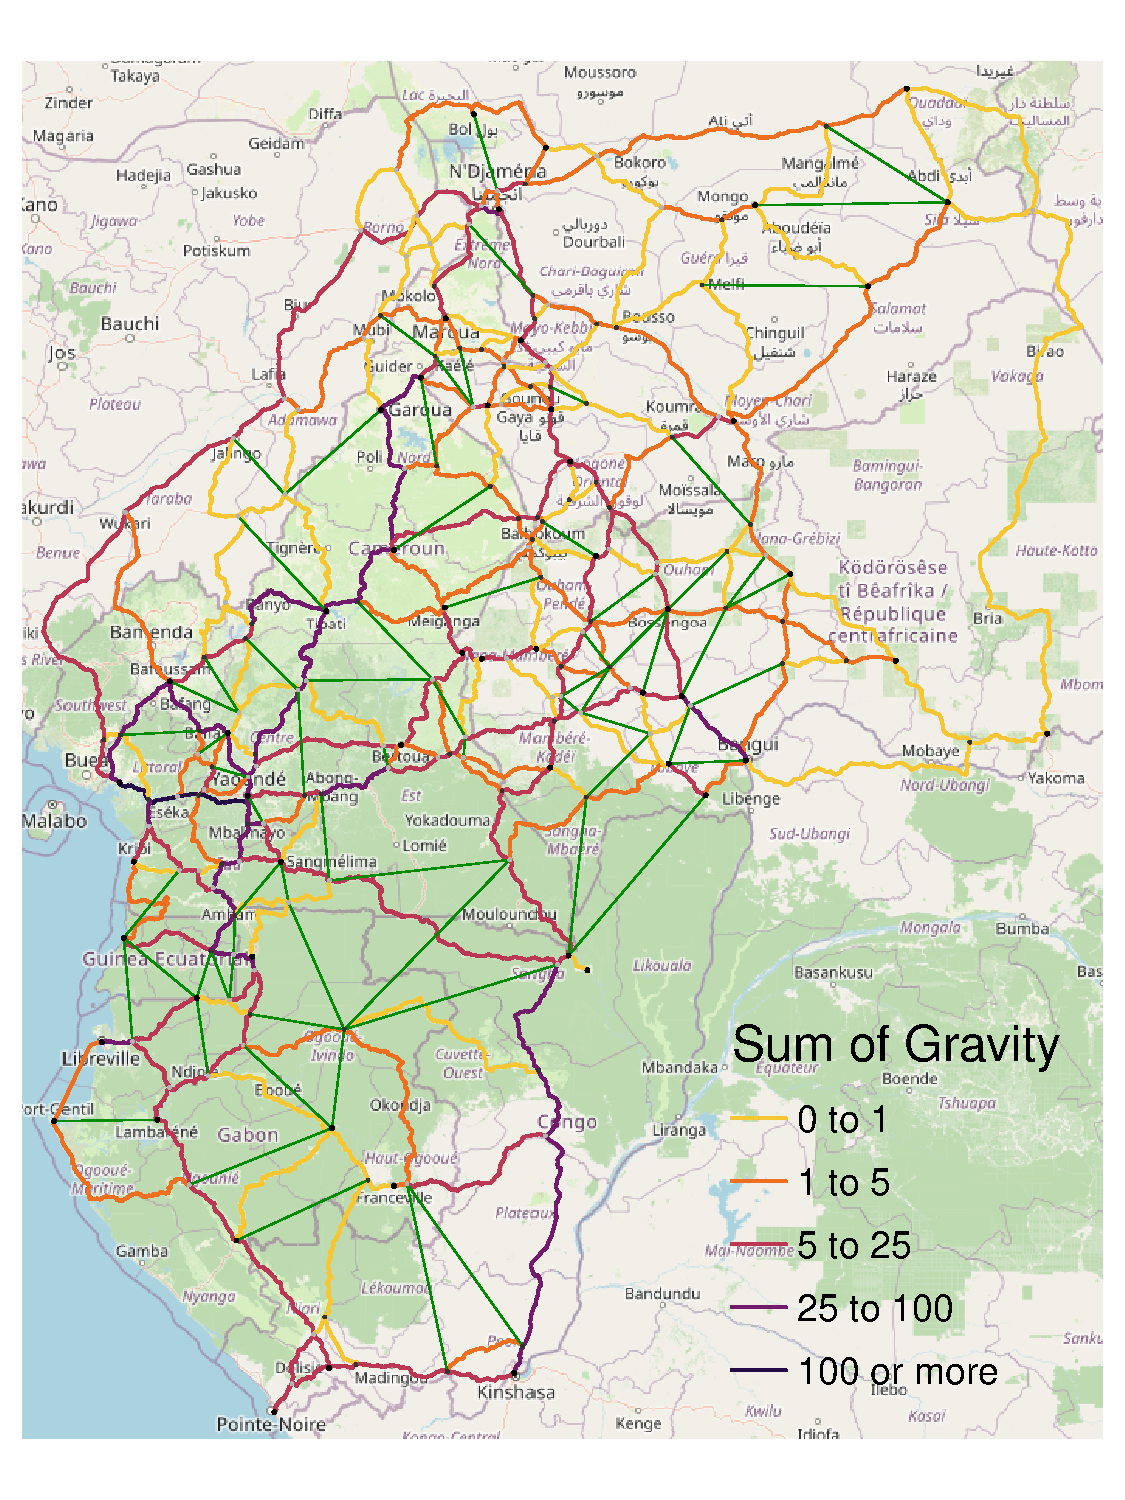
\includegraphics[width=0.48\textwidth]{"../figures/trans_CEMAC_network_actual_discretized_gravity_new_roads_real_edges.pdf"} &
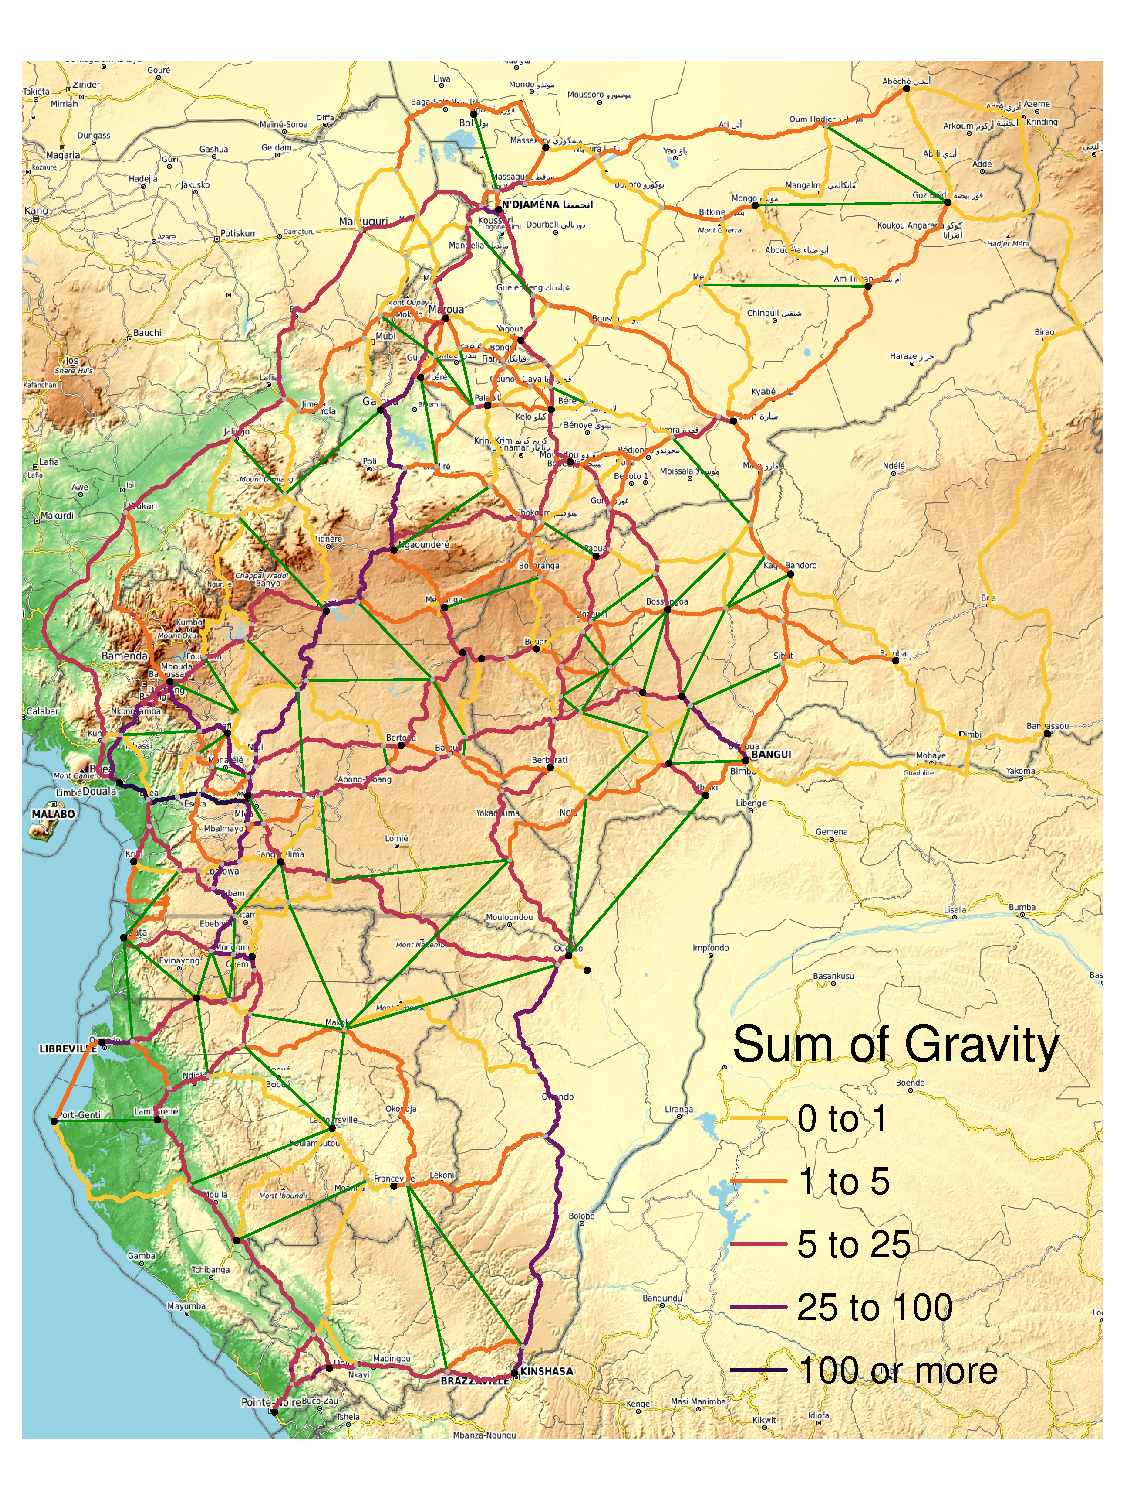
\includegraphics[width=0.48\textwidth]{"../figures/trans_CEMAC_network_actual_discretized_gravity_new_roads_OpenTopoMap.pdf"} \\ [-0.2em]
\end{tabular}
\raggedright
\scriptsize 
\emph{Notes:} Figure shows road network graph against a plain (LHS) and topographic (RHS) background map. The network is obtained from 1431 fastest car routes between 54 cities/agglomerations. Each route is assigned a 'Gravity' estimate amounting to the population (in thousands) of start and end city divided by the road distance in meters. The 'Sum of Gravity' is the sum across all routes using this segment in the network. It is a measure of expected traffic volume. The green lines indicate high-yield network extensions yielding $\geq$50\% reductions in road distance between adjacent nodes. % \\ \vspace{-5mm}
\end{figure}

To parameterize the graph, I add the populations of smaller agglomerations within 30km of these nodes to the node population count, excluding Nigerian agglomerations because CEMAC planners should not maximize welfare or market access in Nigeria. This yields 119 nodes with positive populations, of which 54 are the large cities routed from/to. These nodes account for 80\% of the urban population of CEMAC according to the Africapolis 2025 projection, but only for 45\% of the total population in 2023 according to the World Development Indicators database. Since large cities generally exhibit higher productivities than small cities and rural populations, and, in the absence of a convincing way to measure productivity,\footnote{\citet{krantz2024optimal} in the appendix shows that nightlights per capita is not a convincing productivity measure. \vspace{-3mm}} I make the assumption that they also account for 80\% of the regions GDP. Readers who find this estimate high should note that road projects take 3-5 years to complete, the region's real GDP grew by 2.2\% annually over the last 10 years, and the urban population share, currently at 50\%, is increasing by 0.5 percentage points per year (own calculations using Africa Monitor data \citep{krantz2023africamonitor}). Thus, fixing the GDP of these nodes at 80\% of the region's 2023 GDP (in constant 2015 USD) is moderate for 2028-30.   \newline 

  To better distribute GDP across these nodes, I employ the high-resolution remotely sensed International Wealth Index (IWI) by \citet{lee2022high}. The index estimates asset-based household wealth on a scale from 0 to 100 based on a fixed set of household items recorded in DHS surveys. \citet{lee2022high} combine daylight satellite imagery and OpenStreetMap data in an iterative ML framework to predict the IWI from DHS surveys conducted in 25 Sub-Saharan African (SSA) countries since 2017, and obtain a cross-country $R^2$ of 91.7\%. Their predictions cover all populated areas at an effective resolution of 1.6km. \newline 
  
  To estimate node productivity, I take an inverse-distance-weighted average of all IWI estimates within 10km from each node. This average ranges from $\sim 65$ in port cities such as Port-Gentil, Douala, and Libreville, to $\sim 10$ in some remote cities such as Baibokoum in Chad. I then multiply it with the node population to measure total wealth, and use that to distribute the GDP measure of 80\% of the regions real 2023 GDP, amounting to 72.7 billion 2015 USD (total GDP is \$90.9B), across the 119 populated nodes. \newline 
  
I also take into account cross-border frictions following \citet{krantz2024optimal}. Figure \ref{fig:DB_TAB} visualizes them. The top panel shows the raw border compliance cost and time from the 2019 Doing Business Survey, and the bottom panel shows these converted to road distance and travel time, respectively, also taking into account documentary compliance times/costs. Evidently, and as visible in \citet{krantz2024optimal} Figures 8 and 9, border costs are high in the region, with a median cost of \$2272 and time of 411 hours, compared the African median cost of \$1222 and time of 224 hours. 


  
  
\begin{figure}[H] \vspace{-2mm}
\centering
\caption{\label{fig:DB_TAB} World Bank Doing Business: Border Compliance Frictions in 2019}
\vspace{2mm}
\resizebox{\textwidth}{!}{
\begin{tabular}{cc}
Border Compliance Cost, Median: 2272\$  & Border Compliance Time, Median: 411h \\
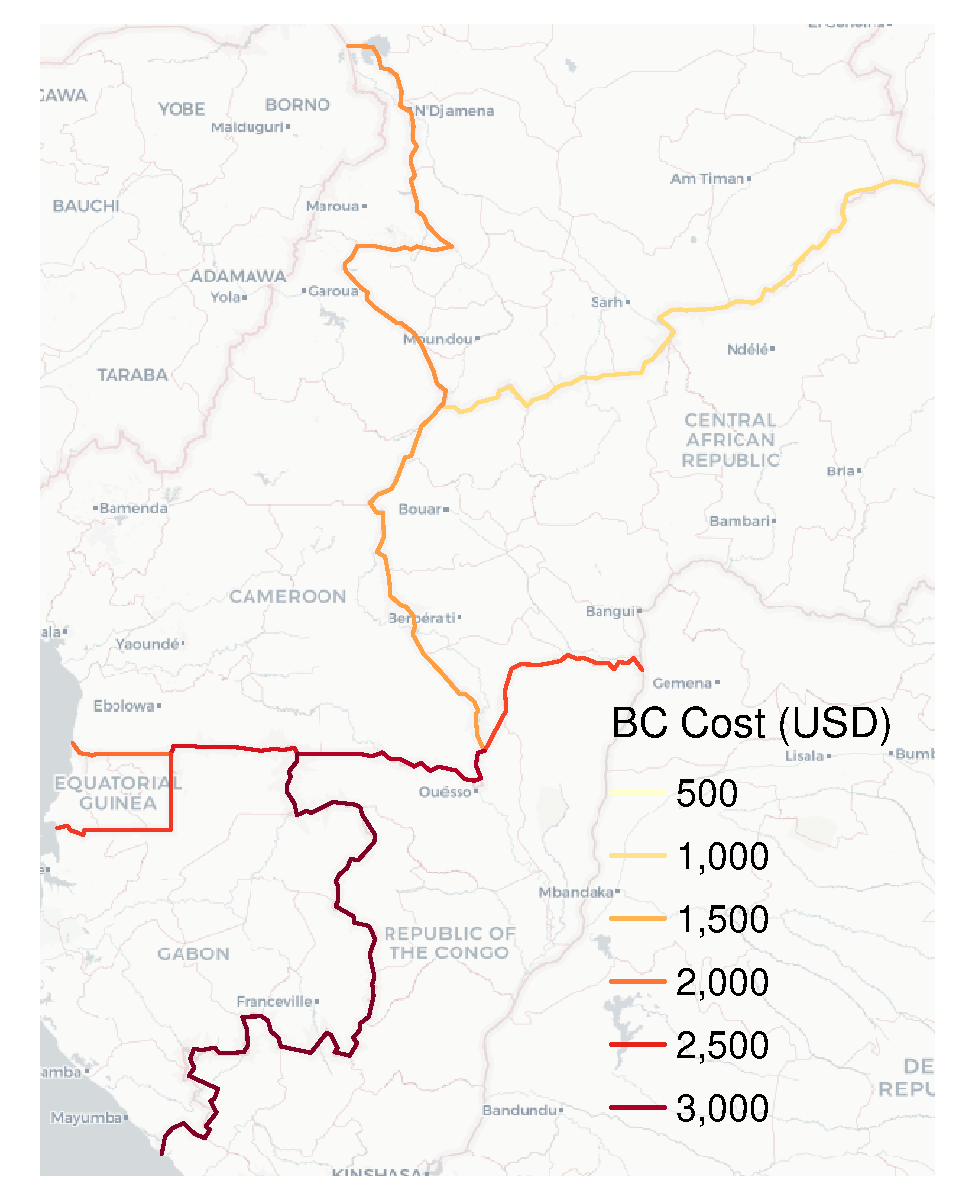
\includegraphics[width=0.5\textwidth, trim= {1cm 0 1cm 0}, clip]{"../figures/trade_costs/DBS_border_cost_usd_map.pdf"}  & 
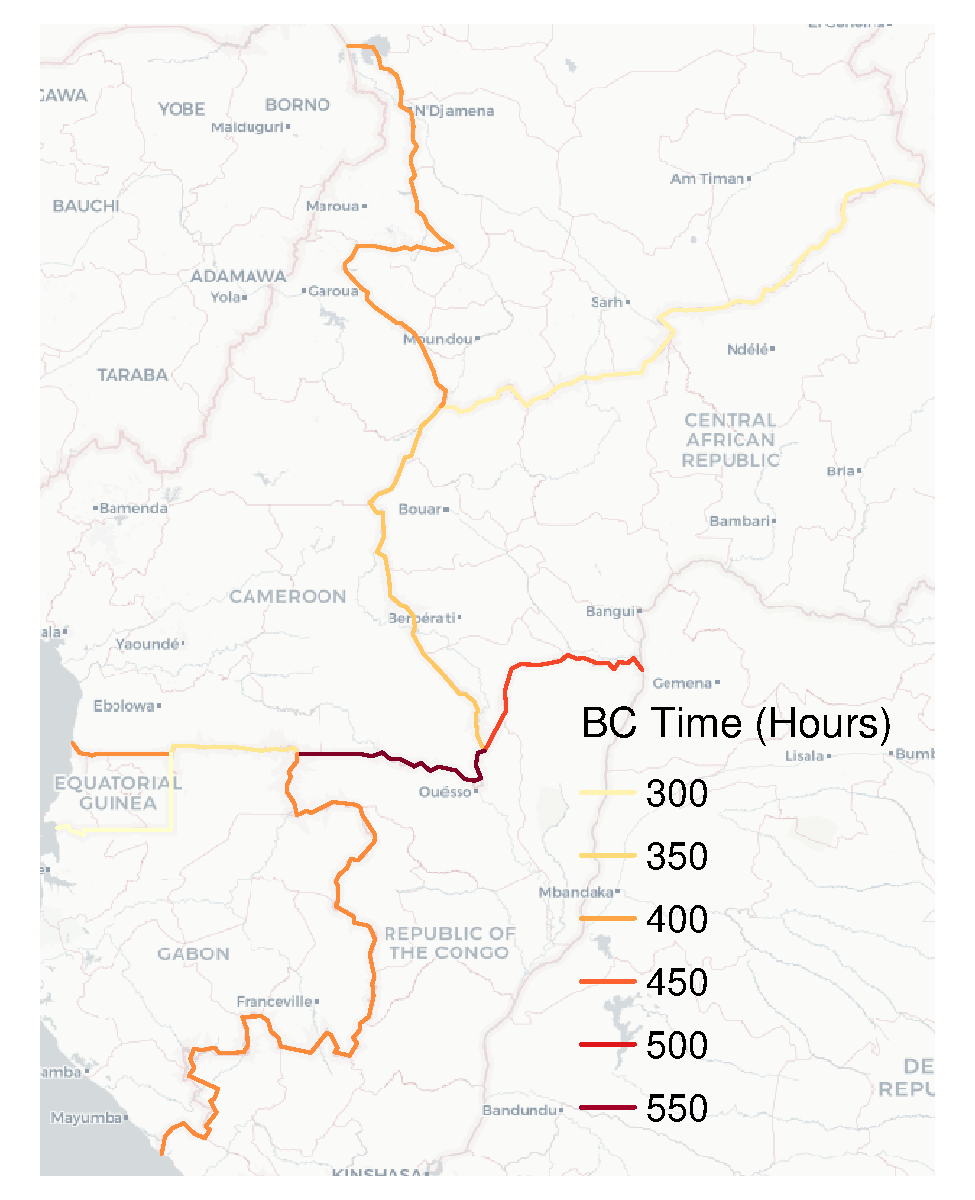
\includegraphics[width=0.5\textwidth, trim= {1cm 0 1cm 0}, clip]{"../figures/trade_costs/DBS_border_time_hours_map.pdf"}  \\ 
Distance-Equivalent Frictions, Median: 1724km & Time-Equivalent Frictions, Median: 127h \\
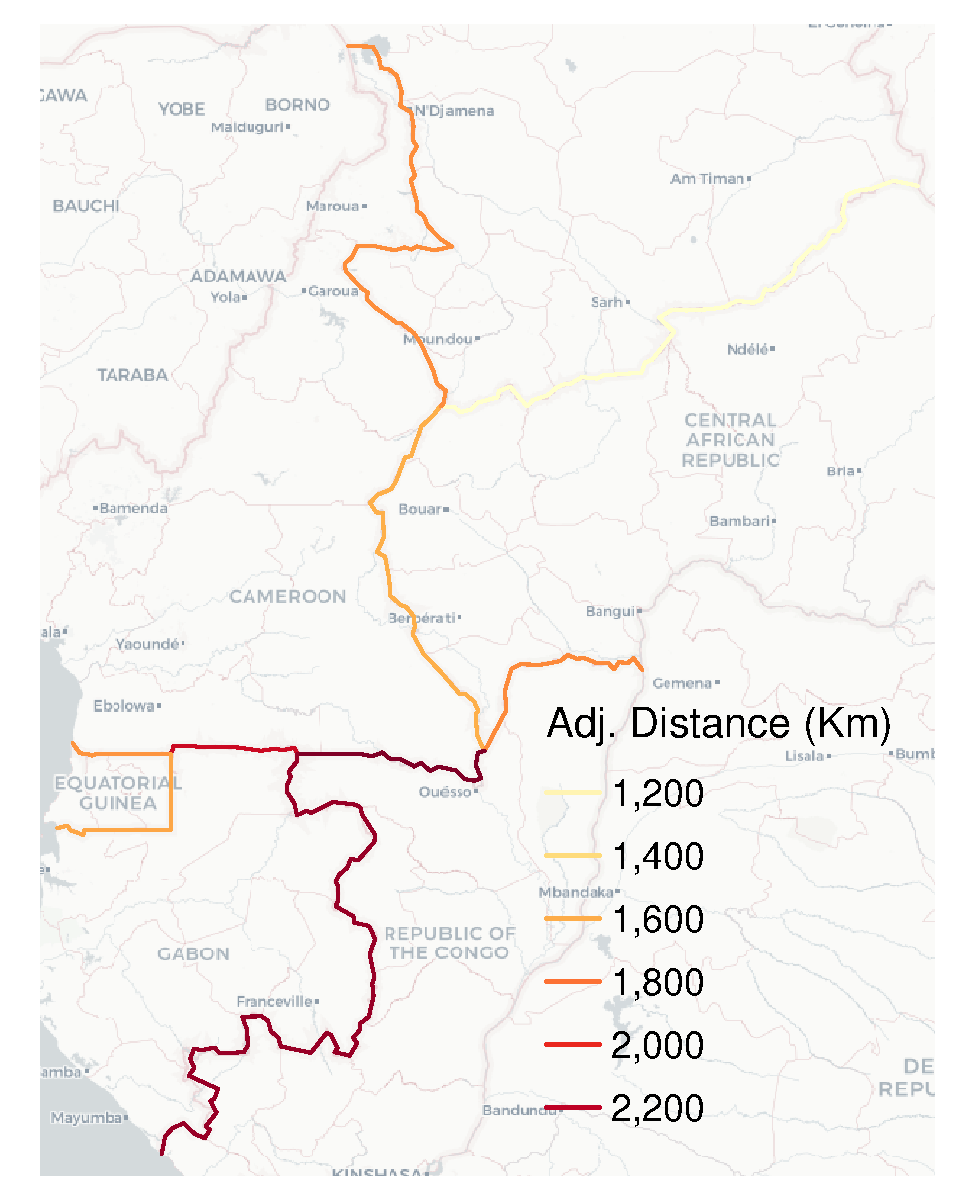
\includegraphics[width=0.5\textwidth, trim= {1cm 0 1cm 0}, clip]{"../figures/trade_costs/DBS_border_dist_km_adj_map.pdf"}  & 
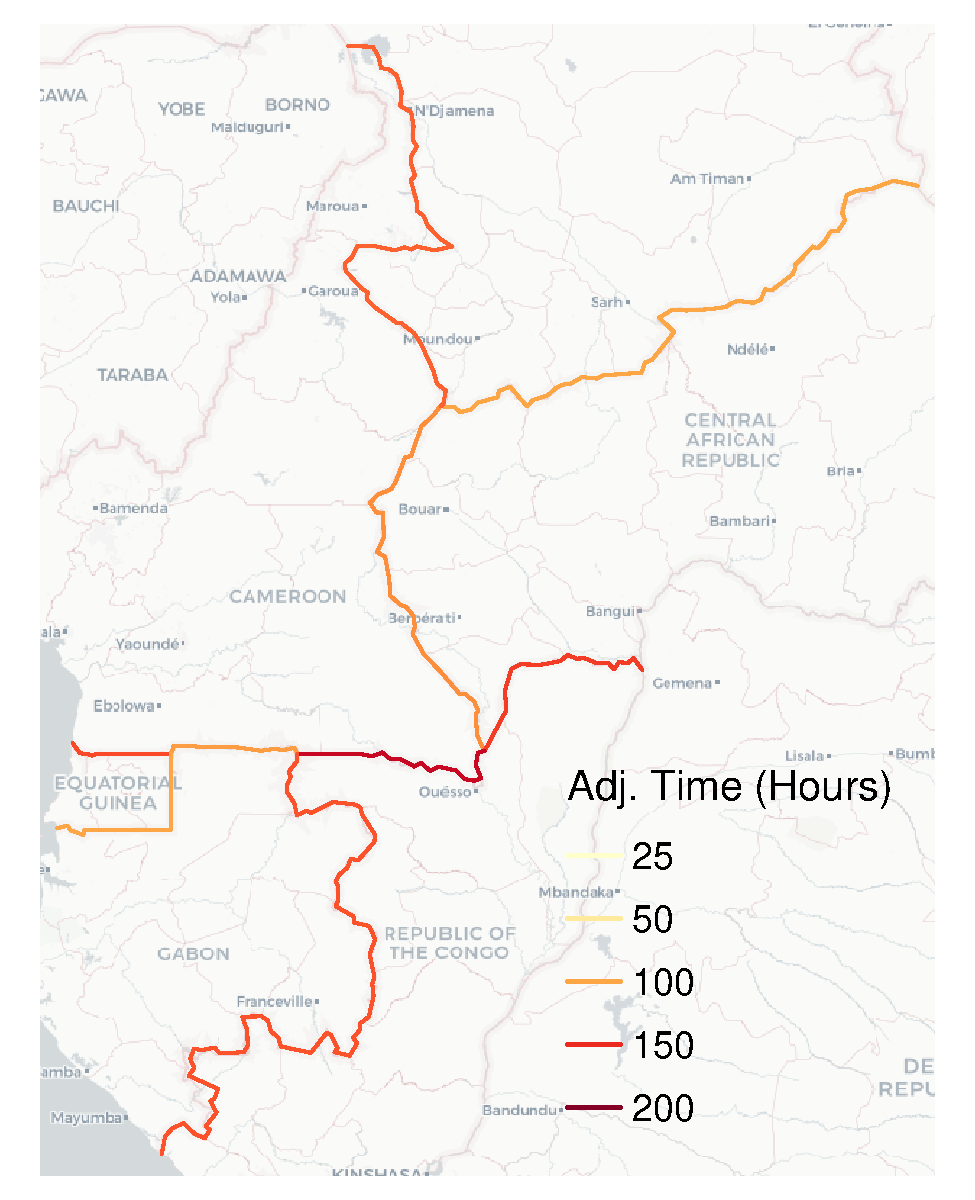
\includegraphics[width=0.5\textwidth, trim= {1cm 0 1cm 0}, clip]{"../figures/trade_costs/DBS_border_time_hours_adj_map.pdf"} \\ [-0.3em] 
\end{tabular}
} 
\raggedright
\scriptsize 
\emph{Notes:} Figure shows average (bi-directional) 2019 border compliance cost/time of trading a standardized product (top panel), and cost/time converted to road distance/travel time following \citet{krantz2024optimal}, i.e., dividing costs by 1.6 and documentary/border times by 10/4, respectively (bottom panel). \vspace{-5mm}
\end{figure}

\newpage
  
  
\section{Optimal Marginal Network Investments}

This section follows \citet{krantz2024optimal} Section 5 by first examining the returns to the proposed new links, then to upgrading existing links, followed by cost-benefit analysis, including joint scenarios. % To limit the scope of exposition, cost-benefit analysis is only done for the joint scenarios. 

\subsection{Building New Links}

The route efficiency (RE) of the network is 0.702, and the RE of the average segment is 0.828. Assuming that the proposed segments (highlighted in green in Figure \ref{fig:ROADS}) also have a RE if 0.828 implies that building all of them increases the NRE by 6.7\% to 0.749. When computing a weighted average of RE across routes using gravity (the product of origin and destination population divided by their geodesic distance) as weights, the weighted NRE measure is 0.718, and building all proposed segments raises it by 4.7\% to 0.753. As in \citet{krantz2024optimal}, the total NRE gain along all optimal routes can also be evaluated individually by segment. Figure \ref{fig:NRE_DA_TAN} shows the percentage gain in NRE from constructing each link. In the unweighted case some large border crossing links in Congo, Gabon, Cameroon and CAR yield high NRE gains, but with gravity weights the most high yield links with a NRE gain of more than 0.5\% are in Ecuatorial Guinea. A look on any street map reveals that the country is not well connected to its neighbours to the north and south.

\begin{figure}[h!] % \vspace{-3mm}
\centering
\caption{\label{fig:NRE_DA_TAN} Percentage Gain in Network RE from Constructing Each Proposed Link}
\vspace{2mm}
\begin{tabular}{cc}
Unweighted NRE Gain (\%) & Gravity Weighted NRE Gain (\%) \\ % Improved US-Grade Network\\
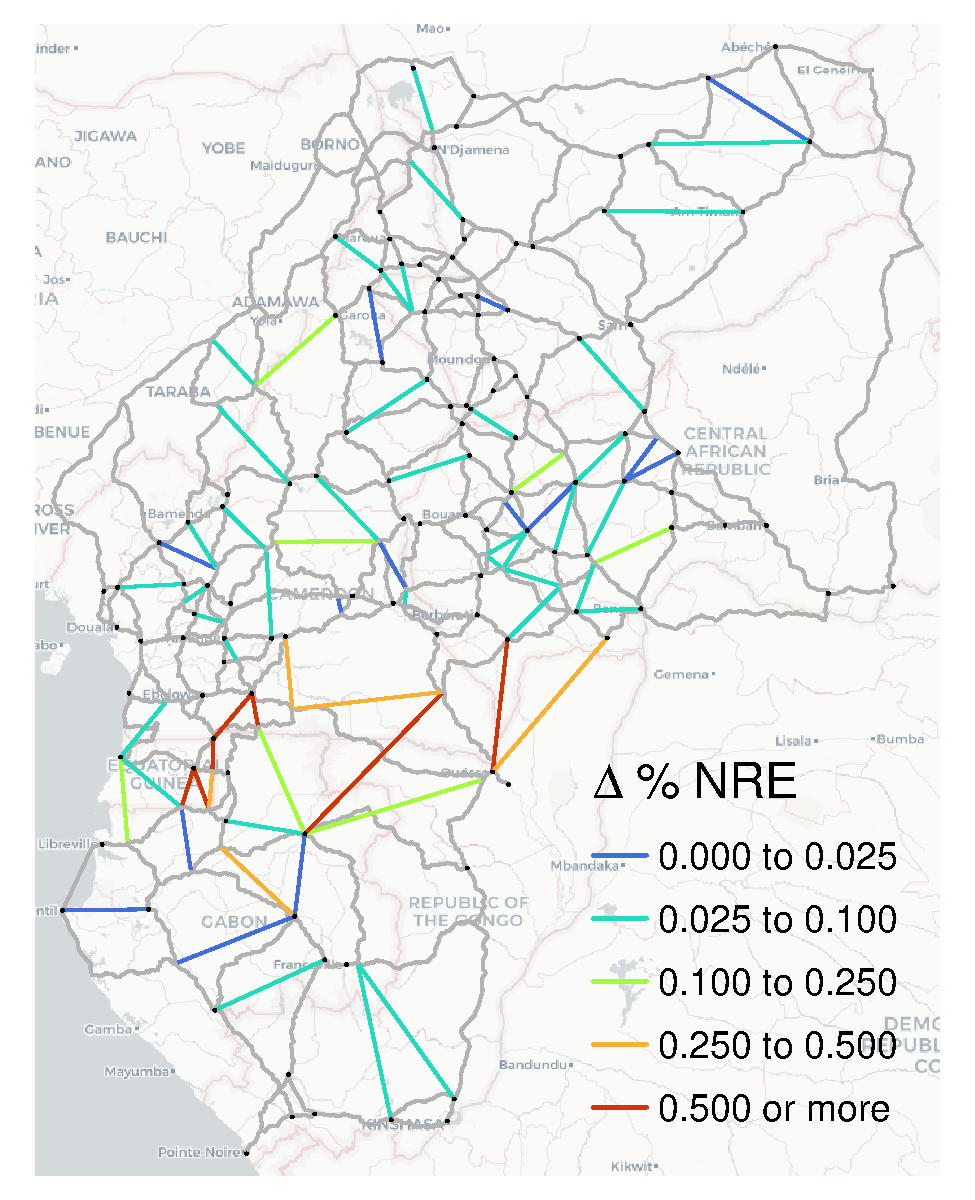
\includegraphics[width=0.48\textwidth]{"../figures/PE/trans_CEMAC_network_NRE_gain_perc.pdf"} &
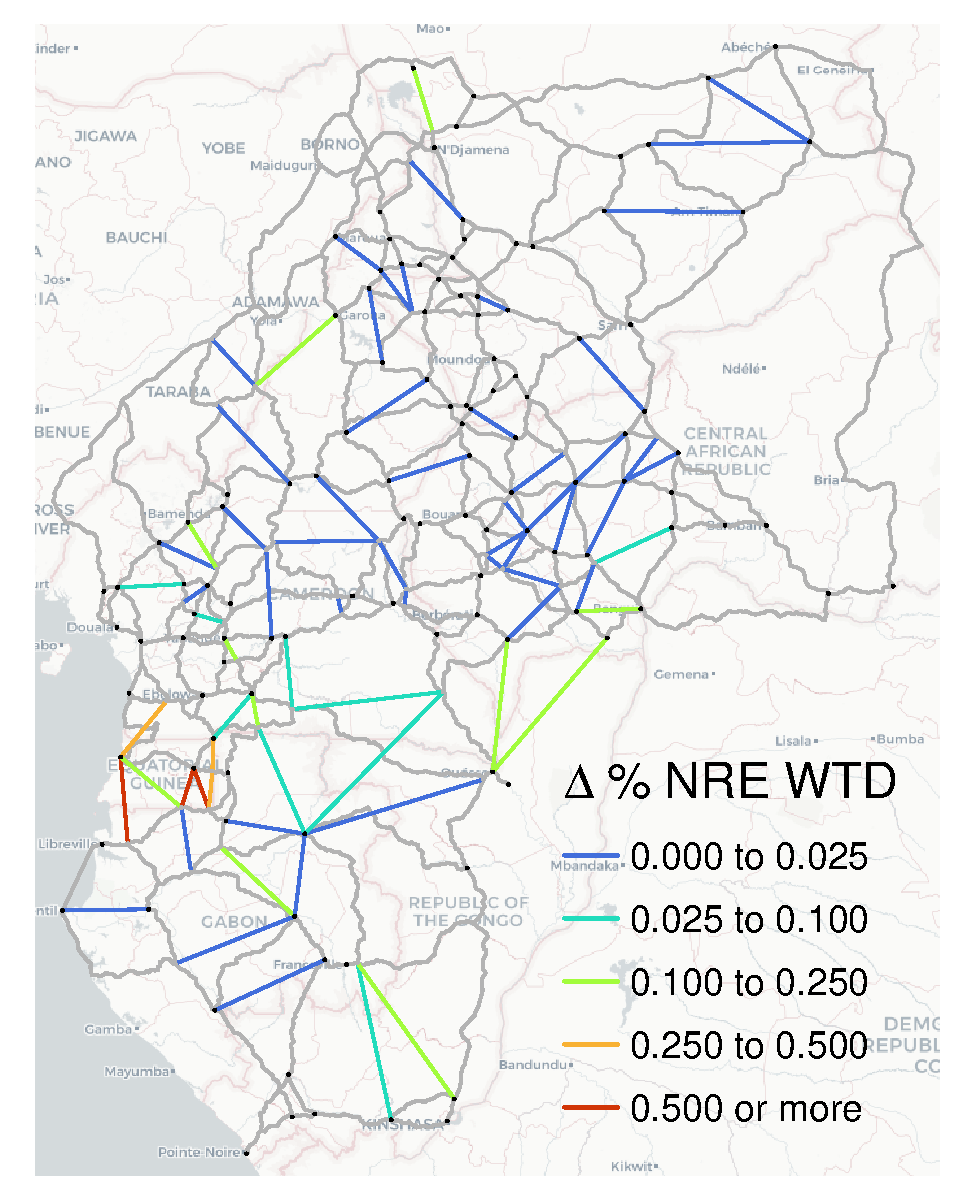
\includegraphics[width=0.48\textwidth]{"../figures/PE/trans_CEMAC_network_NRE_wtd_gain_perc.pdf"} \\ [-0.2em]
\end{tabular}
% \raggedright
\scriptsize 
\emph{Notes:} Figure shows (weighted) average route efficiency (RE) gains across all trips from building a specific link/edge. 
 % \vspace{-1mm}
\end{figure}

Similarly, we can consider total market access (MA) implied by the network, where MA of node $i$ is the sum of the estimated GDP's of all other nodes $j$ divided by their respective road distance along the fastest $i\to j$ route. The total network MA is then the sum of MA across all nodes. The total network MA is 23.1 billion USD'15 per km. Building all proposed links increases MA by 5.2\%. Using 2019 estimates of cross-border frictions from the final edition of the World Bank Doing Business surveys, and translating documentary and border compliance time/cost into road time/distance, respectively, following \citet{krantz2024optimal}, reduces total MA to 16.2 billion USD'15 per km or 30\% smaller. the MA gain from all proposed links reduces to 3\%. Figure \ref{fig:MA_DA_TAN} shows total MA gains from building each link with and without frictions. Ostensibly, frictions reduce the value of new border-crossing links. In fact, the marginal gains from all links are lower under frictions as long as the route is fixed and transiting is less costly.  \citet{krantz2024optimal} discusses other cases where traders can adjust their multi-country routes to minimize border costs, which I refrain from here as the CEMAC region is small. Following \citet{krantz2024optimal}, I set a 48h transit costs (24h per border) for transiting through 3rd countries. %, the focus should not be on the impact of border frictions except to make it clear that they should be removed as much as possible. 


\begin{figure}[H]  \vspace{-1mm}
\centering
\caption{\label{fig:MA_DA_TAN} Percentage Gain in Market Access (GDP) from Constructing Each Proposed Link}
\vspace{2mm}
\begin{tabular}{cc}
No Frictions & 2019 Doing Business Frictions \\
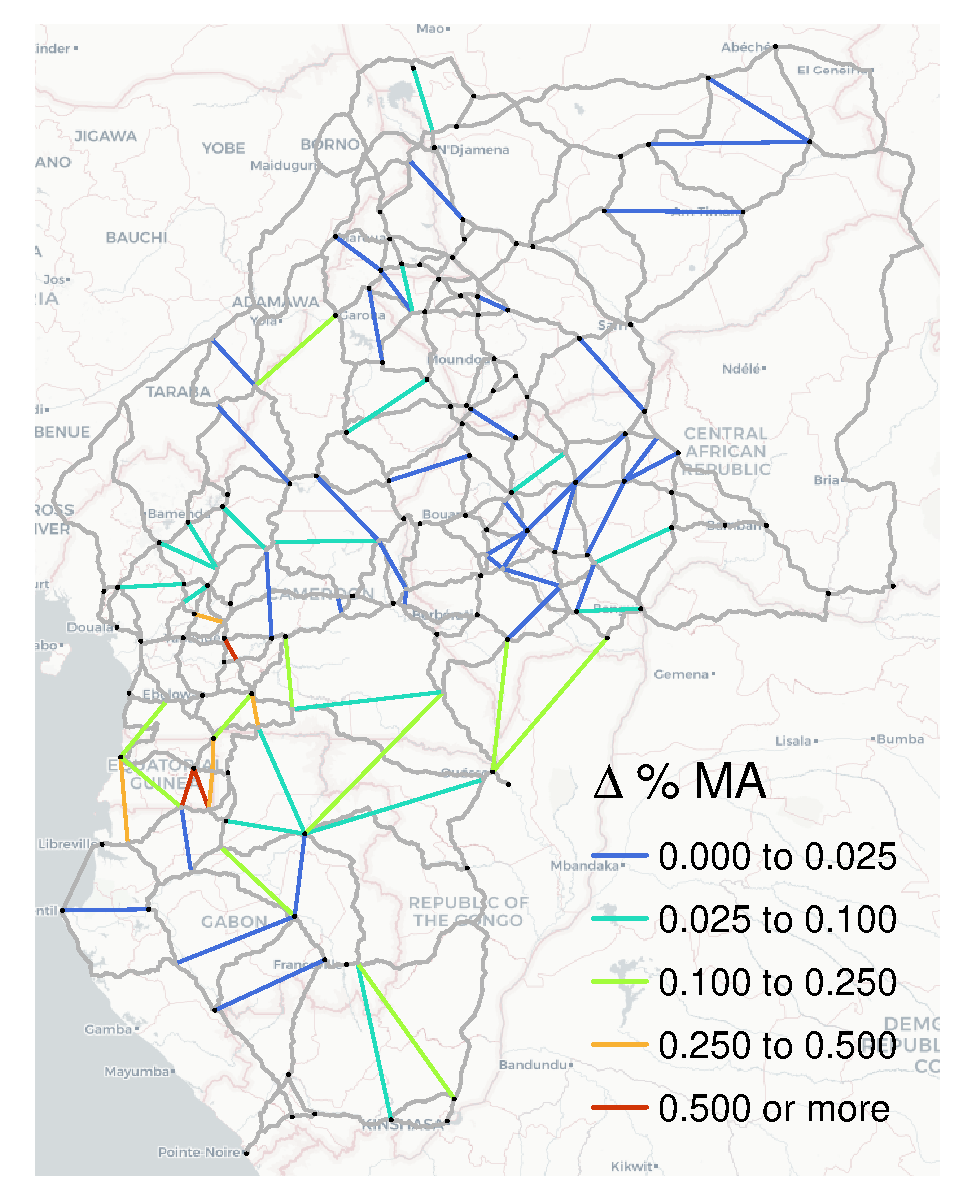
\includegraphics[width=0.48\textwidth]{"../figures/PE/trans_CEMAC_network_MA_gain_perc.pdf"} &
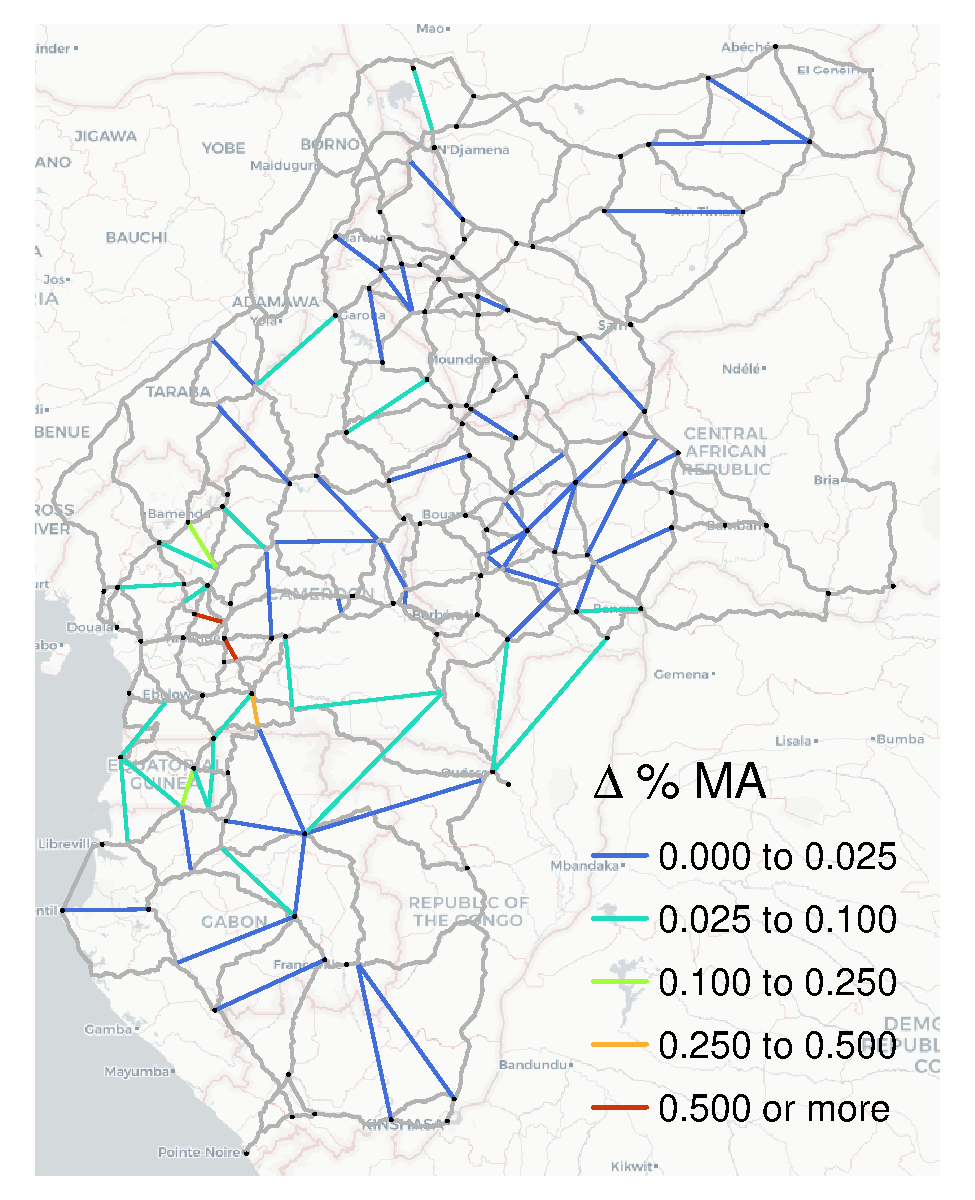
\includegraphics[width=0.48\textwidth]{"../figures/PE/trans_CEMAC_network_MA_gain_perc_bc.pdf"}  \\ [-0.2em]
\end{tabular}
% \raggedright
\scriptsize 
\emph{Notes:} Figure shows total road-distance denominated MA gains measured (summed) across all trips from building a link. 
 % \vspace{-2mm}
\end{figure}

\subsection{Upgrading Existing Links}

The median link speed, taken from Google Maps without traffic awareness, is 60km/h, ranging from 6.2km/h for the slow ferry connection from Libreville to Port-Gentil, to 103km/h on the highway from Bata to Mongomo in Equatorial Guinea. Figure \ref{fig:ALS} shows the speed of each link. 

\begin{figure}[H]  \vspace{-1mm}
\centering
\caption{\label{fig:ALS} Average Link Speed}
\vspace{2mm}
\begin{tabular}{cc}
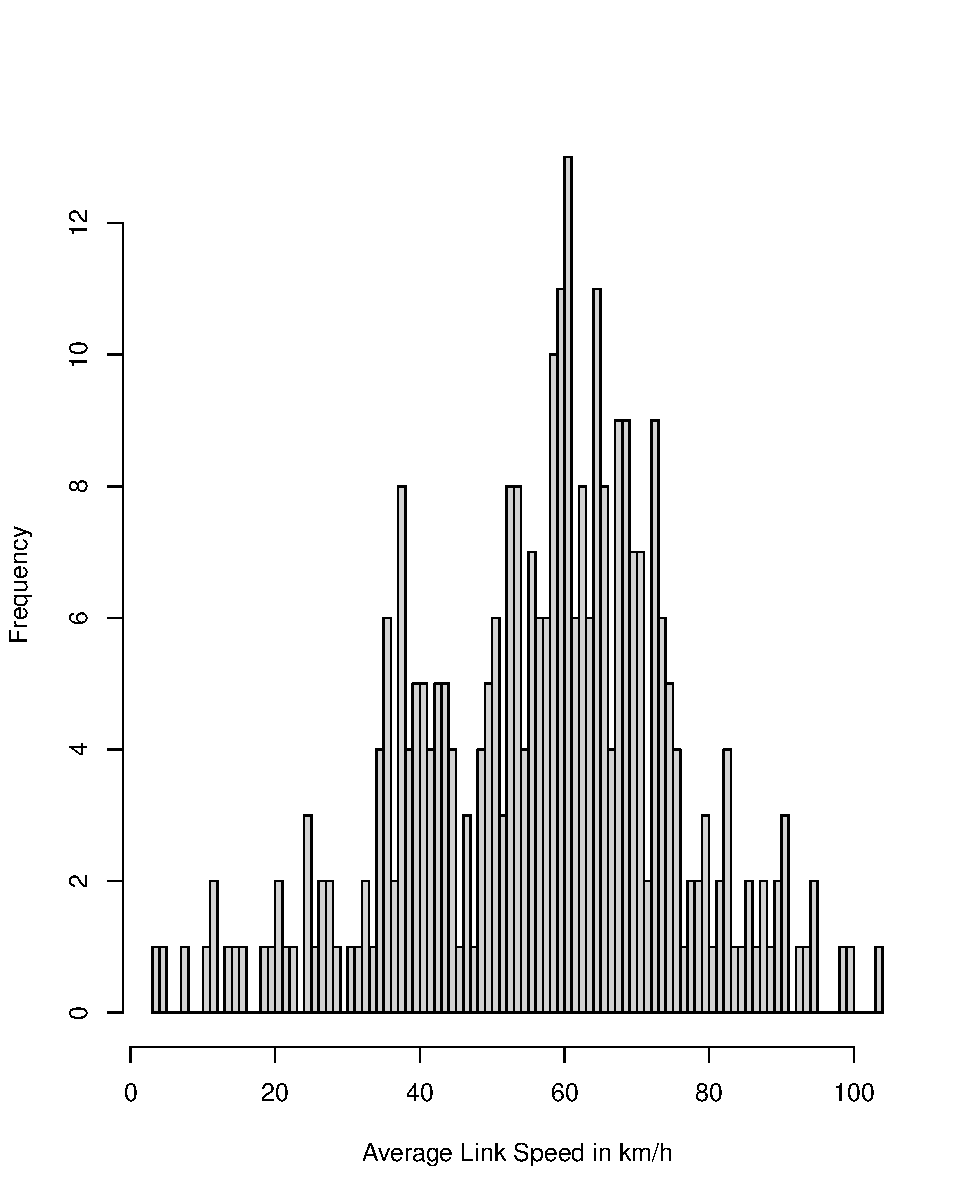
\includegraphics[width=0.48\textwidth, trim = {0 0.4cm 1.5cm 2.5cm}, clip]{"../figures/trans_CEMAC_network_average_link_speed_hist_google.pdf"} &
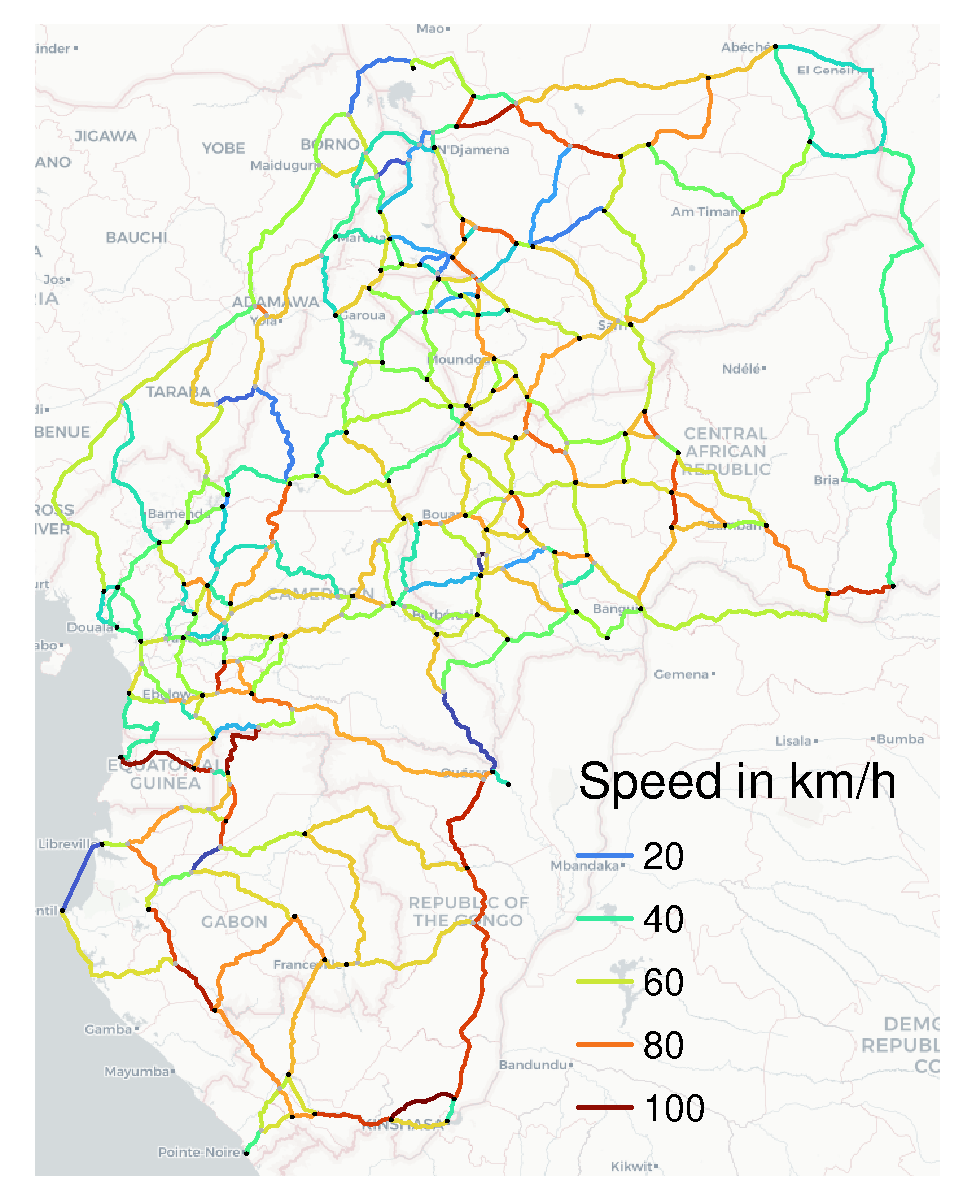
\includegraphics[width=0.48\textwidth]{"../figures/trans_CEMAC_network_average_link_speed_google.pdf"}  \\ % [-0.2em]
\end{tabular}
% \raggedright
\scriptsize 
\emph{Notes:} Figure shows the average speed along each link, estimated via Google Maps API without traffic awareness. 
\end{figure}

The total travel-time-denominated MA implied by the network is 20.6 billion USD'15 per minute. Upgrading all roads to allow travel speeds of 100km/h, raises total MA by 81.2\%. Under border frictions the MA drops to 12.1 billion USD'15 per minute or 40.8\% smaller, and the gains from upgrading all roads is 77.4\%. Figure \ref{fig:MA_TT} shows the gains from upgrading each link individually. 

% Total MA gains from building at 100km/h and upgrading 30.57% or 9.31 billion USD'15/min

\begin{figure}[H]  \vspace{-1mm}
\centering
\caption{\label{fig:MA_TT} Percentage Gain in Market Access from Upgrading Each Link to $\geq$100km/h}
\vspace{2mm}
\begin{tabular}{cc}
No Frictions & 2019 Doing Business Frictions \\
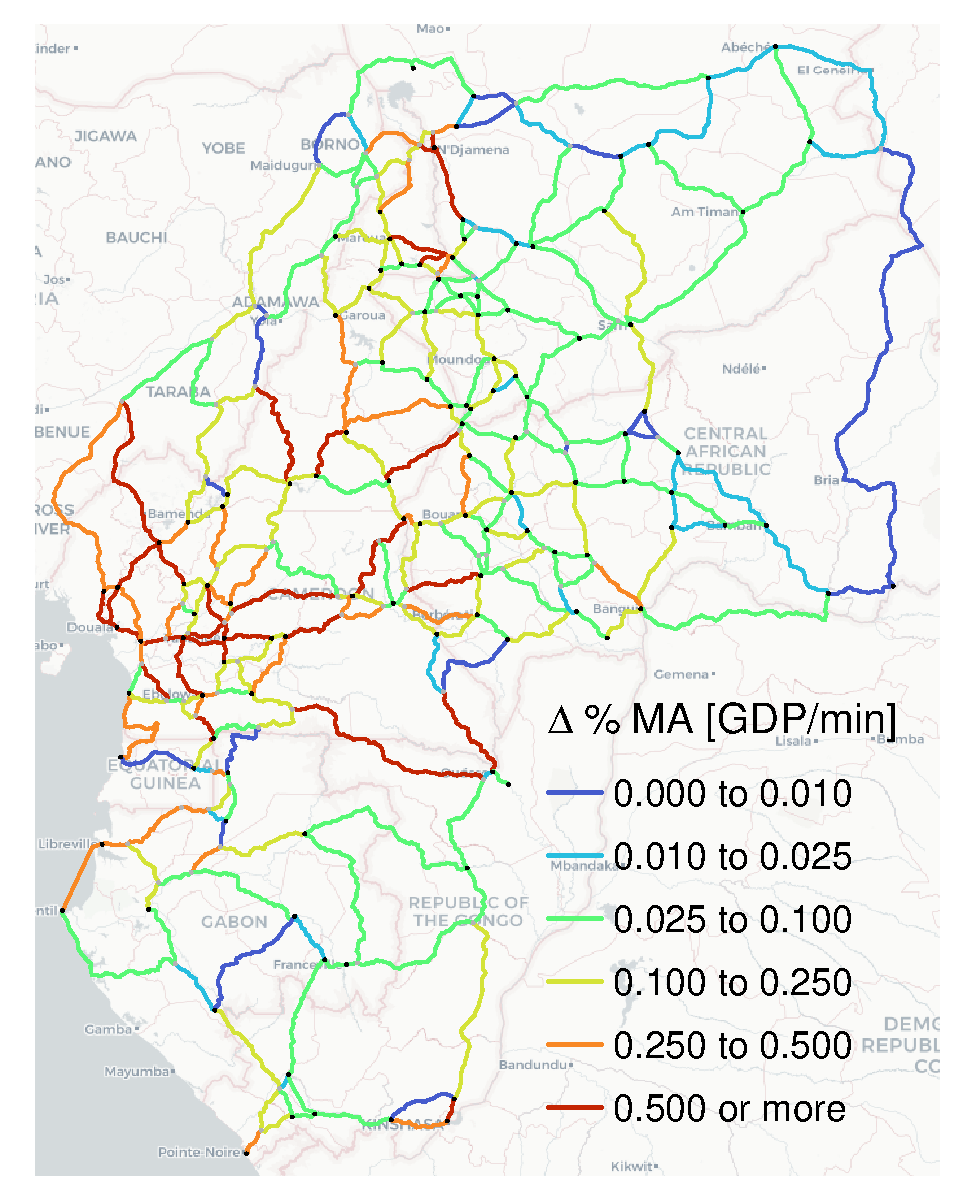
\includegraphics[width=0.48\textwidth]{"../figures/PE/trans_CEMAC_network_MA_100_min_speed_perc_google.pdf"} &
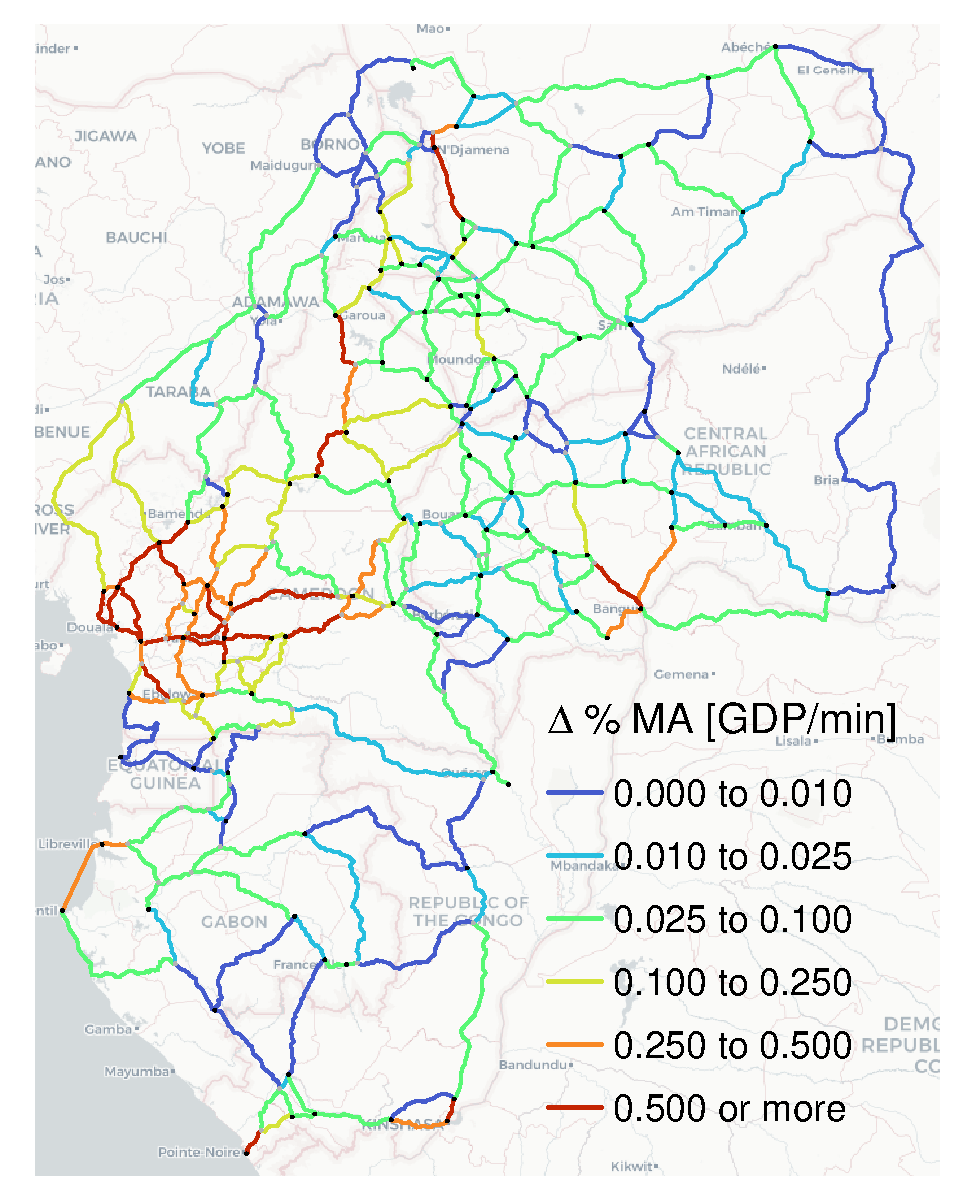
\includegraphics[width=0.48\textwidth]{"../figures/PE/trans_CEMAC_network_MA_100_min_speed_bt_perc_google.pdf"}  \\ [-0.2em]
\end{tabular}
\raggedright
\scriptsize 
\emph{Notes:} Figure shows total travel-time-denominated MA gains measured (summed) across all trips from upgrading a link to allow travel speeds of $\geq$100km/h. 
 % \vspace{-2mm}
\end{figure}

Ostensibly, upgrading links in the populated areas of Cameroon, the by far largest economy among the 6, yields the greatest MA returns, especially under border frictions. Without frictions, better connecting the economic center of Cameroon up north and east also yields high MA gains.  

\subsection{Cost-Benefit Analysis}

To decide in which roads to invest, the cost of building roads must be taken into consideration. Following \citet{krantz2024optimal}, which in turn follows \citet{collier2016cost} using the updated Road Cost Knowledge System (ROCKS) database, I allow for heterogeneity in road construction costs. The median cost of a 2-lane highway in SSA is \$611K/km (2015 USD). This is consistent with recent data from the CEMAC region yielding a median cost of \$614K/km and median rehabilitation cost of \$356K/km. I follow \citet{fajgelbaum2020optimal} and \citet{graff2024spatial} and only consider average returns to ruggedness and distance, as well as population. My preferred specification is 
\begin{equation} \label{eq:COST}
\ln\left(\frac{\text{cost}}{km}\right) = \ln(X) -0.11 \times (\text{dist} > 50km) + 0.12 \times \ln(\text{rugg}) + 0.085 \times \ln\left(\frac{\text{pop}}{km^2}+1\right),
\end{equation}
where $X$ = 120,000 for new roads, $X$ = 101,600 for upgrades, $X$ = 64,600 for mixed works, and $X$ = 28.400 for resurfacing. The first part is taken from Eq. (21) of \citet{fajgelbaum2020optimal}, the population coefficient follows \citet{collier2016cost} and \citet{krantz2024optimal}. The 120,000 USD/km constant makes the mean cost/km across all existing links in Africa approximately equal to \$611K/km, and the other thresholds adjust for different kinds of upgrading costs following \citet{krantz2024optimal}: (1) roads with travel speed $<$60km/h require an upgrade at average cost of \$513K /km; (2) roads with travel speeds of 60-79km/h require mixed works at average cost of \$326K/km; (3) roads with travel speeds of 80-90km/h require resurfacing at \$143K/km on average. \newline 

Figure \ref{fig:RUGG_POP} shows ruggedness from \citet{nunn2012ruggedness} and WorldPop 2020 population density, both are estimated within a 3km two-sided buffer around existing and new links. Ostensibly, the area around Bamenda in Cameroon, and further north along the Cameroon-Nigeria border is very rugged. This area is also conflict prone$-$Appendix Figure \ref{fig:ACLED} shows ACLED conflict event data \citep{raleigh2023political}. \citet{collier2016cost}'s road cost prediction model also includes a conflict variable suggesting that costs rise by 20\% during times of violence, but this is not considered in Eq. \ref{eq:COST}. Areas around major cities, especially Douala and Yaounde, are highly populated. 

\begin{figure}[H] \vspace{-1mm}
\centering
\caption{\label{fig:RUGG_POP} Ruggedness and Population Density within 3km Buffer around Links}
\vspace{2mm}
\begin{tabular}{cc}
Ruggedness \citep{nunn2012ruggedness} & Population Density (WorldPop 2020) \\
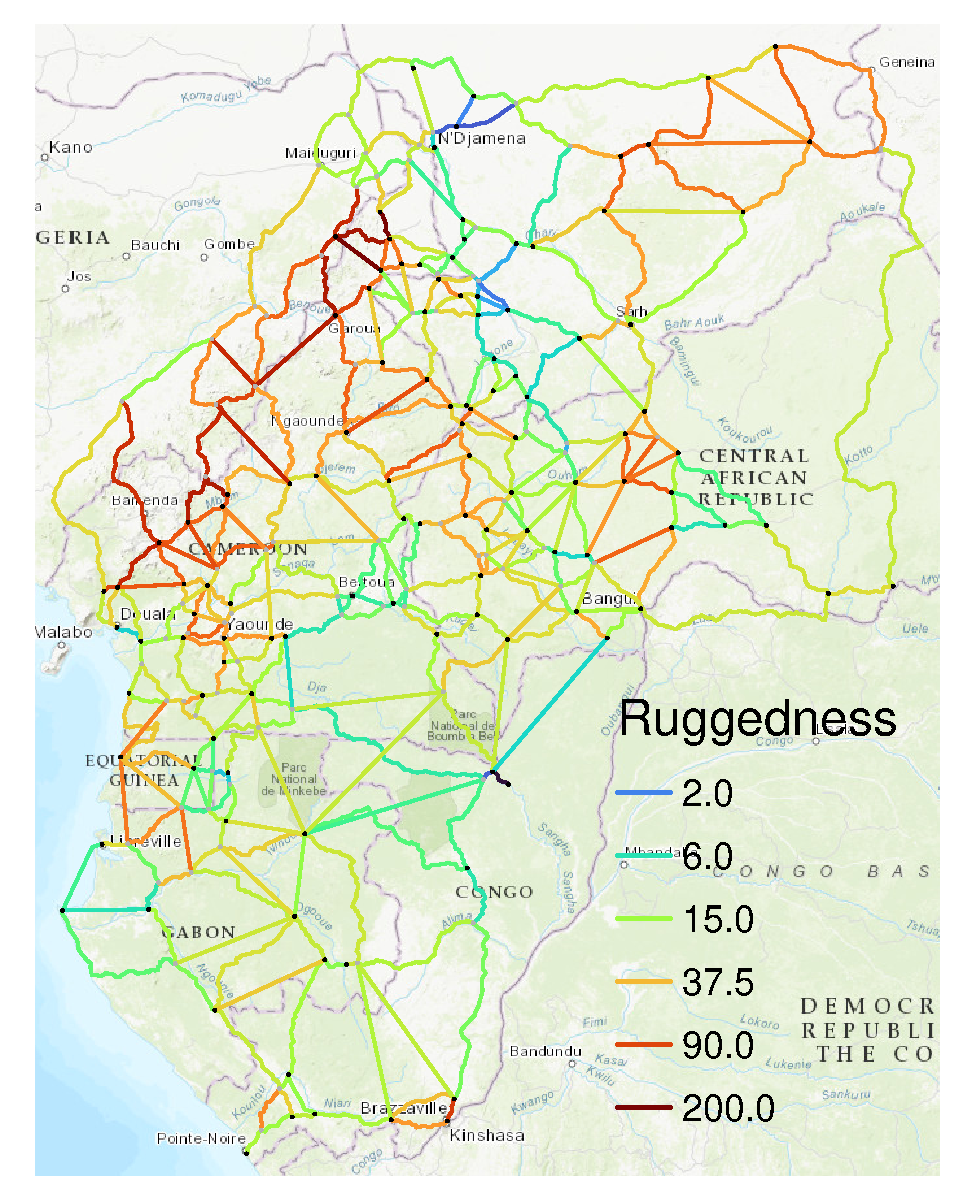
\includegraphics[width=0.48\textwidth]{"../figures/trans_CEMAC_network_rugg.pdf"} &
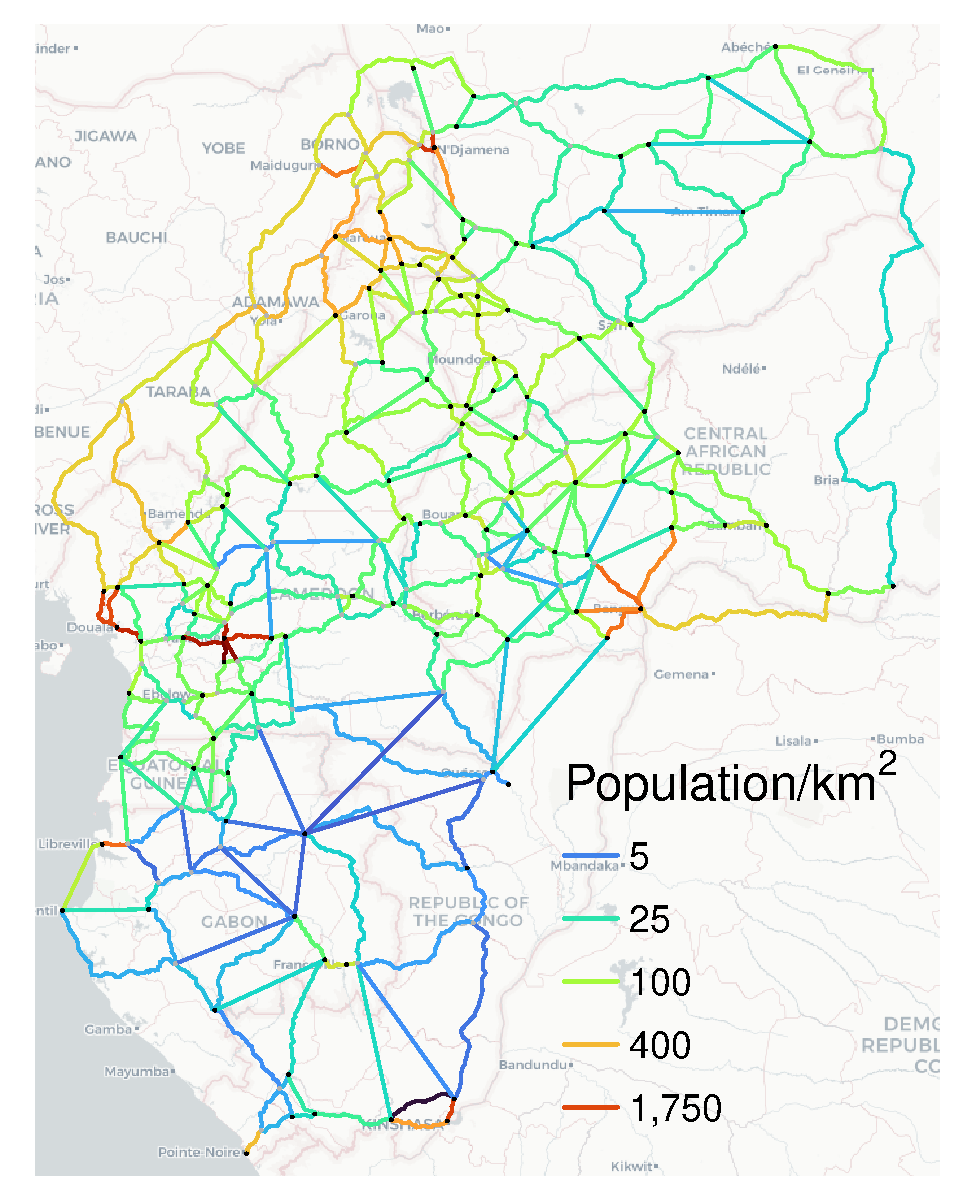
\includegraphics[width=0.48\textwidth]{"../figures/trans_CEMAC_network_pop_wpop_km2.pdf"} \\ [-0.2em]
\end{tabular}
% \raggedright
\scriptsize 
\emph{Notes:} Figure shows average ruggedness and total population within a 3km (two-sided) buffer around links.
% \vspace{-2mm}
\end{figure}


Figure \ref{fig:CTW} shows the different types of work and their estimated costs. Total network cost is 19.9 billion USD'15, and all proposed links cost 6.4 billion USD'15. Total upgrading cost is 13.5 billion USD'15, of which 0.21 billion is resurfacing, 3.97 billion mixed works, and 9.31 billion upgrades. 

\begin{figure}[H] \vspace{-1mm}
\centering
\caption{\label{fig:CTW} Type of Work and Cost}
\vspace{2mm}
\begin{tabular}{cc}
Type of Upgrading Work & Cost Per Km \\
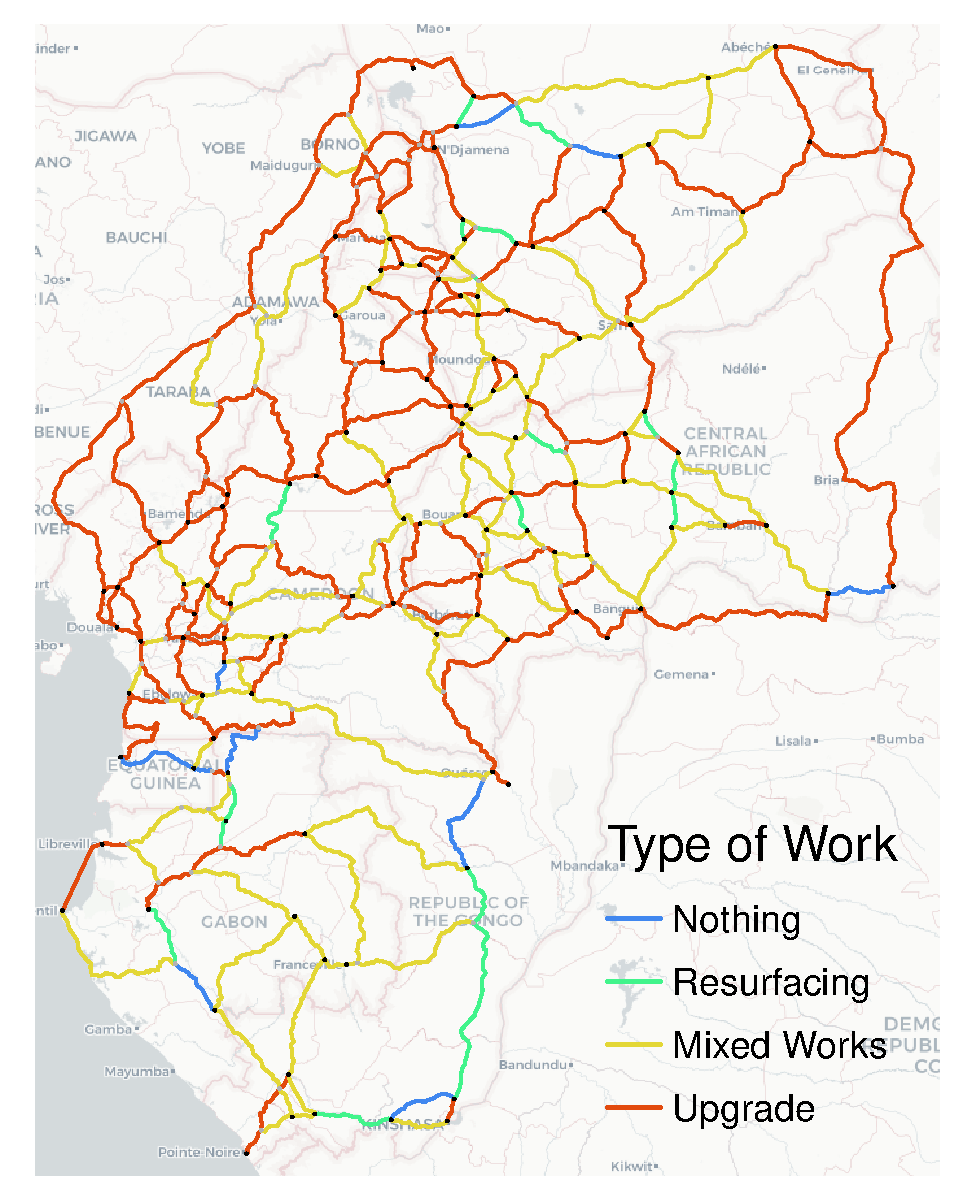
\includegraphics[width=0.48\textwidth]{"../figures/trans_CEMAC_network_type_of_work_google.pdf"} &
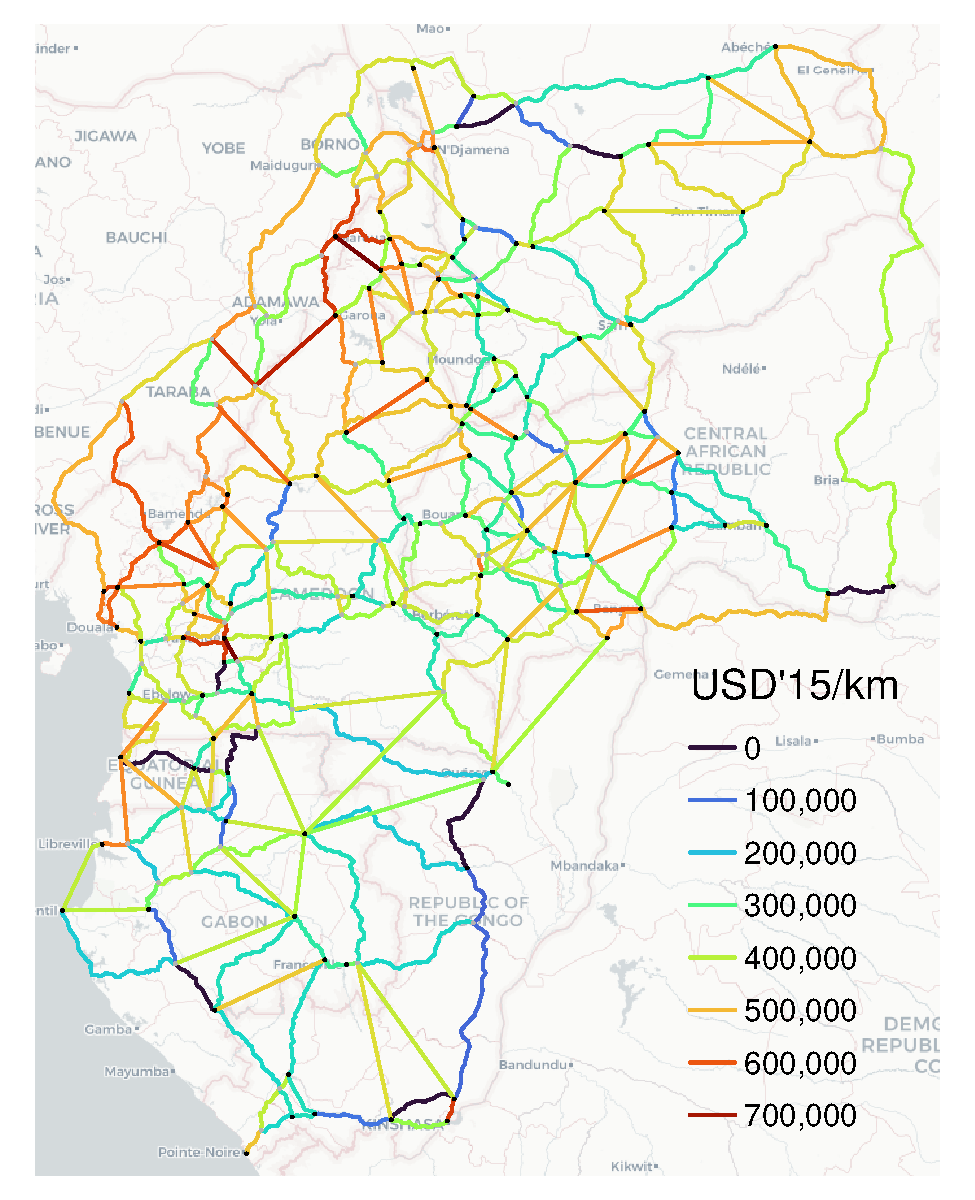
\includegraphics[width=0.48\textwidth]{"../figures/trans_CEMAC_network_all_costs_google.pdf"} \\ [-0.2em]
\end{tabular}
% \raggedright
\scriptsize 
\emph{Notes:} Figure shows the type of work depending on link speed: links $<$60km/h need upgrading, between 60 and 80km/h need mixed works, and links 80-90km/h need resurfacing. Links above 90km/h do not need additional work. \\ \vspace{-0.5cm}
\end{figure}

Following \citet{krantz2024optimal}, I compute link-level cost-benefit ratios as the gain in MA divided by the cost, yielding estimates denominated in \$/min/\$ or 'dollar per minute per dollar invested'. The economic value if such a metric depends on how increases in MA translate into increases in economic activity.  \citet{donaldson2016railroads}'s estimates of railroad-induced increases in MA on US land values between 1870 and 1890 suggest that MA translates into economic activity at a rate of 2:1, however, the contemporary African context may be very different. Readers should also note that, particularly in comparison with \citet{krantz2024optimal}, the focus on the CEMAC region alone yields smaller estimates of MA gains from road projects because locations outside of CEMAC which could benefit from them, including traders transiting through CEMAC, are not considered. \newline 

The average gain from upgrading existing links to allows speeds of 100km/h is 1.19\$/min/\$. This drops to 0.67\$/min/\$ under border frictions. In either case, \citet{donaldson2016railroads}'s finding would imply that economic gains are at max half of that, thus upgrading all links is not sensible. Only 17.2\% of links have gains above 2\$/min/\$ without frictions, indicating medium-term profitability. With frictions only 8.6\% have gains above 2\$/min/\$. \newline 

Figure \ref{fig:MA_PUSD} shows these marginal gains across all links. The yellow and orange links indicate potential medium-term profitability. It is notable that, except for two small segments in the vicinity of Yaounde, no proposed link is medium-term profitable under the frictions scenario. However, without frictions, new links to better connect Equatorial Guinea are medium-term profitable. 

\begin{figure}[H]  \vspace{-1mm}
\centering
\caption{\label{fig:MA_PUSD} Investment Returns in \$/min/\$ from Building/Upgrading Each Link to $\geq$100km/h}
\vspace{2mm}
\begin{tabular}{cc}
No Frictions & 2019 Doing Business Frictions \\
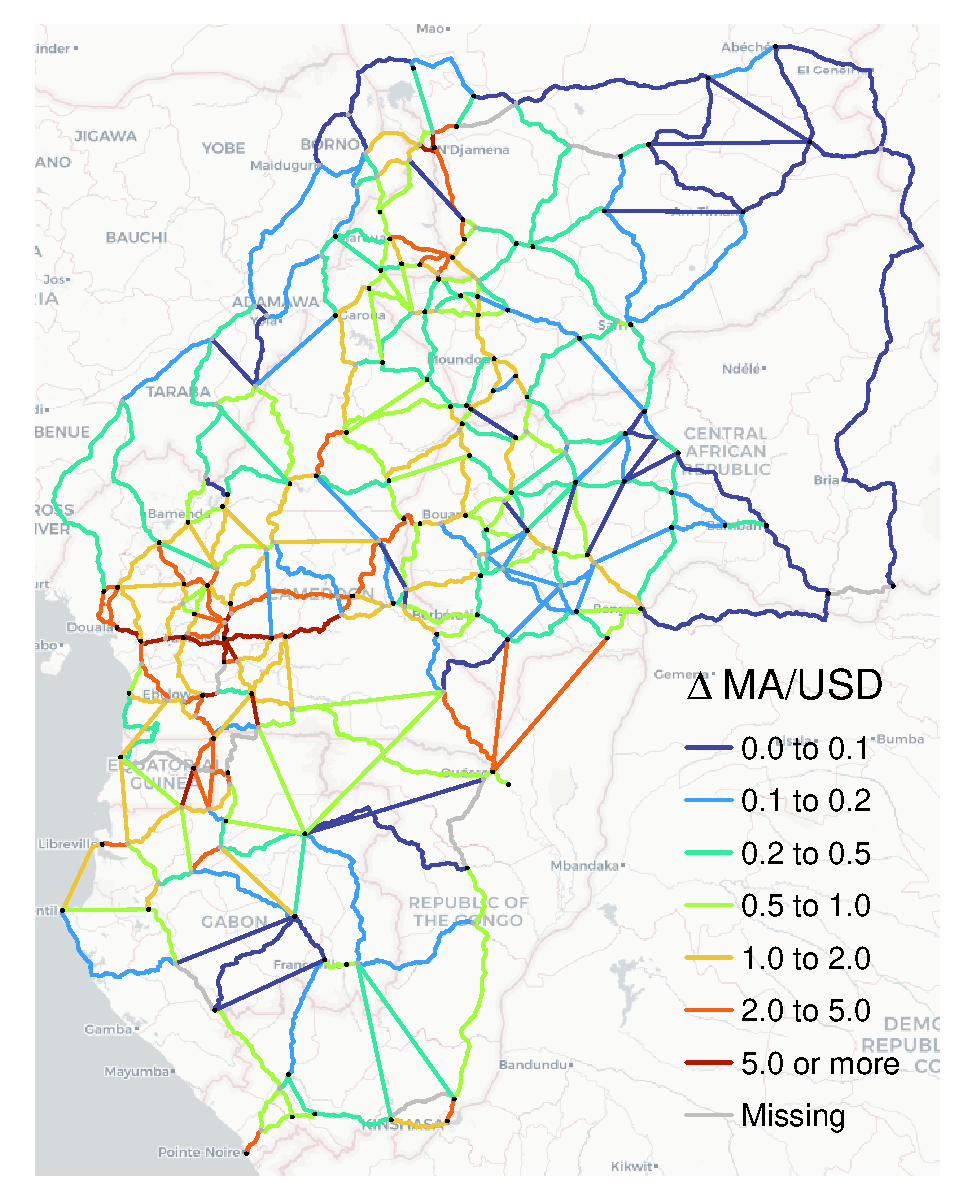
\includegraphics[width=0.48\textwidth]{"../figures/PE/trans_CEMAC_network_MA_gain_all_100kmh_pusd_google.pdf"} &
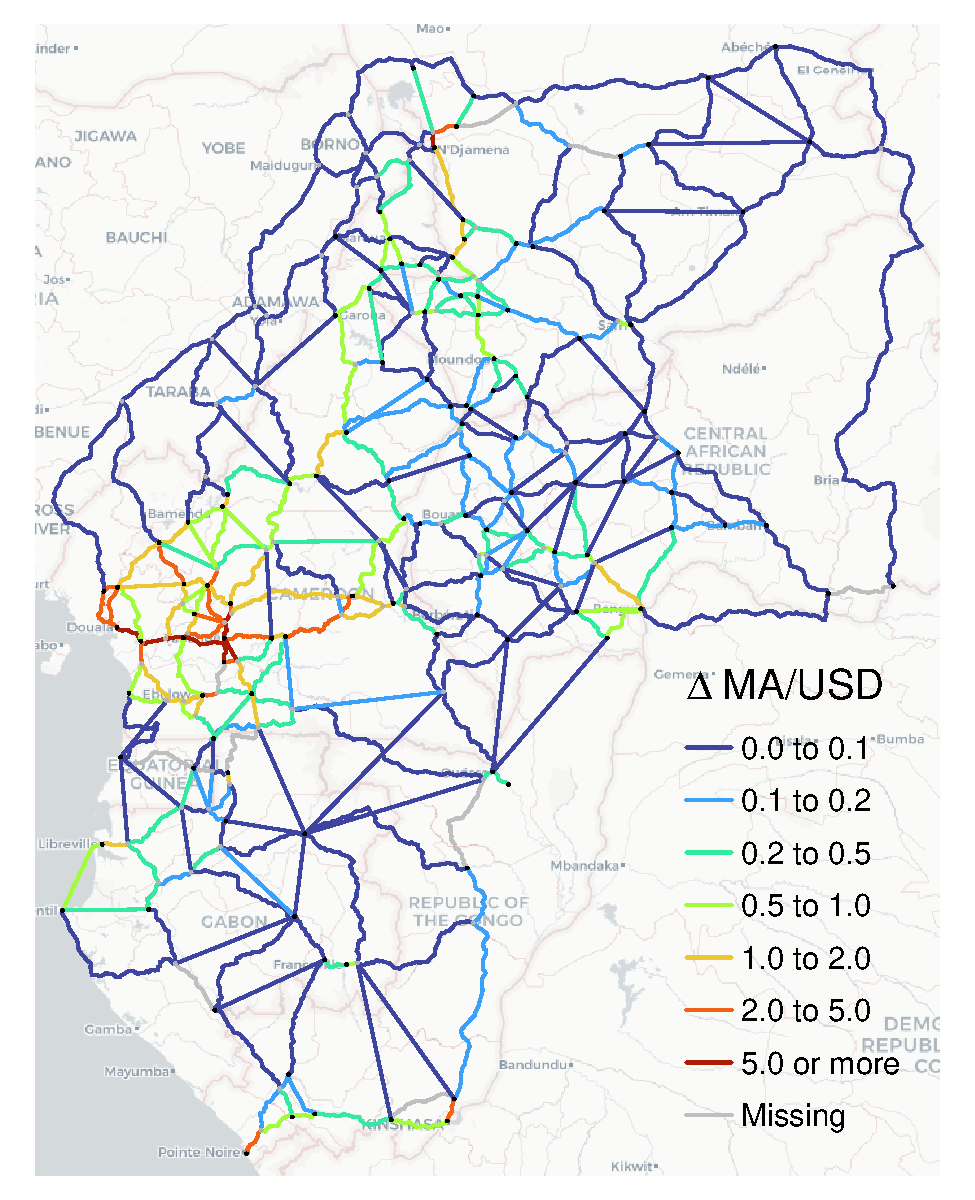
\includegraphics[width=0.48\textwidth]{"../figures/PE/trans_CEMAC_network_MA_gain_all_100kmh_pusd_bt_google.pdf"}  \\ [-0.2em]
\end{tabular}
\raggedright
\scriptsize 
\emph{Notes:} Figure shows marginal returns in \$/min/\$ (dollar per minute $=$ MA per dollar invested) from upgrading a link to allow travel speeds of $\geq$100km/h or building a new link. New links, indicated as straight lines, are assumed to be 1.208x longer than their geodesic distance $\to$ the inverse of the average route efficiency of 0.828 across existing links in the region.  
 % \vspace{-2mm}
\end{figure}


A good policy is thus to build/upgrade high-yield links along with lesser yield links for guaranteed positive returns. For example one could select all links with a marginal return above 0.5\$/min/\$ with or without border frictions, the average return (across frictions/no frictions) of which is shown on the LHS of Figure \ref{fig:UG_cons}. It includes 18.3\% of the length of all existing network and 6.6\% of all proposed link lengths. Building/upgrading these costs 1.72 billion USD'15 and yields a 17.1\% MA gain, amounting to 5.2 billion USD'15/min or 3.02\$/min/\$. Under frictions the MA gain drops to 3.82 billion USD'15/min or 2.21\$/min/\$. This package may be profitable if we are optimistic about project costs and/or frictions being reduced (or potentially already much lower than in 2019). \newline 

A more prudent package would consider all links with a marginal return above 1\$/min/\$ with or without border frictions, the average return of which is shown on the RHS of Figure \ref{fig:UG_cons}. It includes 13.8\% of the length of all existing network and 1.65\% of all proposed link lengths. Building/upgrading these costs 3.31 billion USD'15 and yields a 55\% frictionless MA gain, amounting to 10.9 billion USD'15/min or 3.3\$/min/\$. Under frictions the MA gain drops to 8.28 billion USD'15/min or 2.5\$/min/\$. 

 % This package may be profitable if we are optimistic about frictions being reduced, or potentially already much lower than in 2019.

% yields a joint MA gain (after recalculating all shortest paths) of 12.9\% without frictions, amounting to \$3.91 billion or 4.25\$/min/\$. Under border frictions, the MA gain drops to \$2.97 billion or 3.22\$/min/\$. 

\begin{figure}[H] \vspace{-1mm}
\centering
\caption{\label{fig:UG_cons} Consensus Packages: High-Yield Links with or without Frictions}
\vspace{2mm}
\begin{tabular}{cc}
All links $>$0.5\$/min/\$ & All links $>$1\$/min/\$ \\
% \includegraphics[width=0.48\textwidth]{"../figures/PE/trans_CEMAC_network_MA_gain_100_min_speed_pusd_cons.pdf"} &
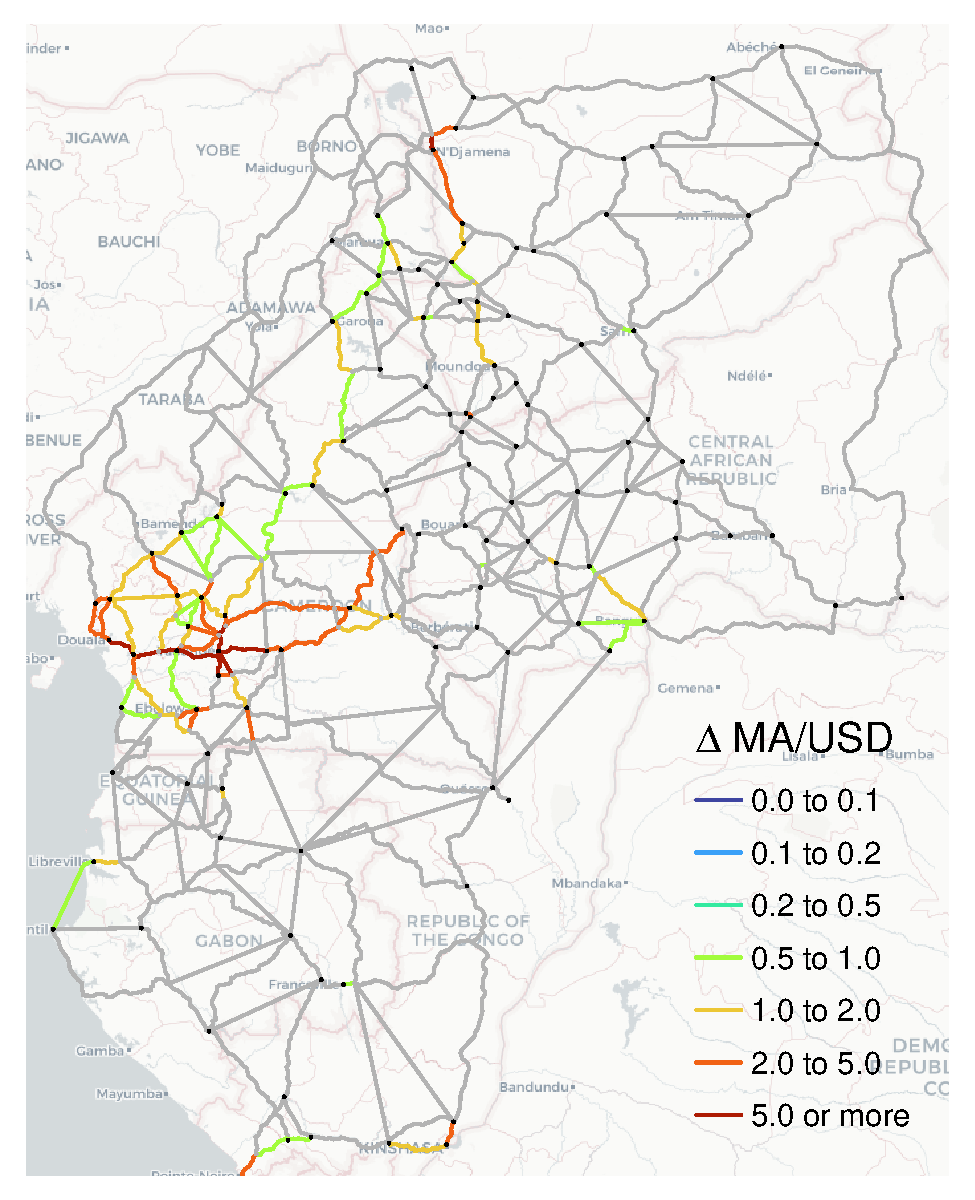
\includegraphics[width=0.48\textwidth]{"../figures/PE/trans_CEMAC_network_MA_gain_all_100kmh_pusd_cons_MAg0.5_google.pdf"} &
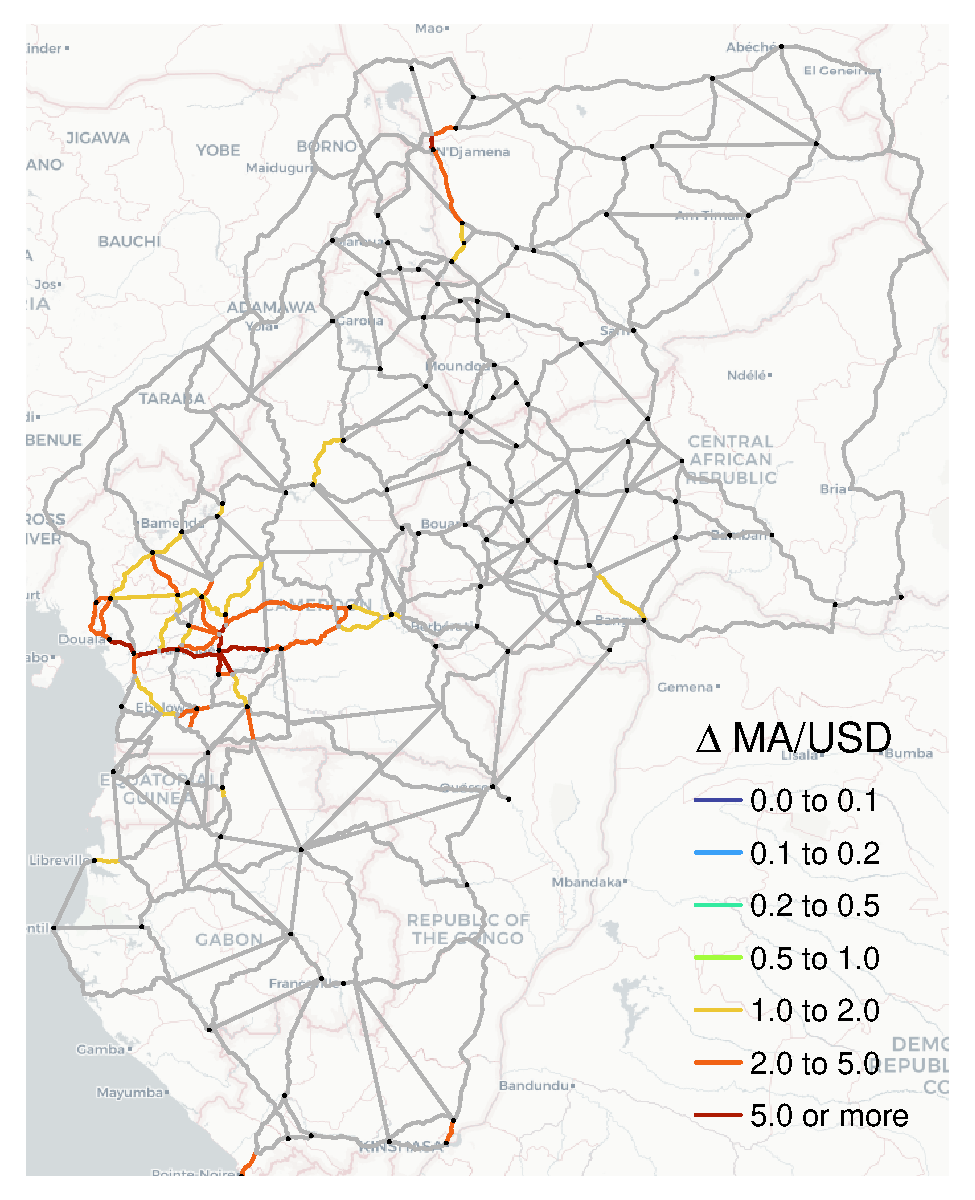
\includegraphics[width=0.48\textwidth]{"../figures/PE/trans_CEMAC_network_MA_gain_all_100kmh_pusd_cons_MAg1_google.pdf"} 
% \includegraphics[width=0.48\textwidth]{"../figures/trans_CEMAC_network_upgrading_costs.pdf"} \\ [-0.2em]
\end{tabular}
% \raggedright
\scriptsize 
\emph{Notes:} Figure shows the average marginal returns to building/upgrading selected links across the frictions and no frictions scenarios. These links have marginal gains above the threshold value with and without border frictions.  
\end{figure}

We could also take only high-yields above 2\$/min/\$ marginal gains. This includes only 4.4\% of the length of all existing network and 1.04\% of all proposed link lengths. Building/upgrading these costs 0.84 billion USD'15 and yields a 32\% frictionless MA gain, amounting to 6.4 billion USD'15/min or 7.6\$/min/\$. Under frictions gains drops to 5.48 billion USD'15/min or 6.5\$/min/\$. \newline 

In the absence of frictions, significantly larger investment packages (e.g., all light green and orange/red links in the LHS of Figure \ref{fig:MA_PUSD}) are potentially profitable. To make a realistic assessment, more accurate information about border frictions and economic returns to MA in the region are needed. MA maximization is also not a redistributional policy, but planners may have legitimate redistributional objectives and clear budget constraints. The condition of roads and their upgrading costs may also not be very accurately captured by routing engines and calibrated remote sensing estimates following \citet{collier2016cost} and \citet{fajgelbaum2020optimal}. Thus, knowledge of the region and its road network, and engineering constraints, must also be considered. \newline 

A final assessment regards macroeconomic feasibility in present-discounted-value (PDV) terms. Here, I also follow \citet{krantz2024optimal} and consider the minimum increase in the macroeconomic growth rate from each package necessary to break even after 30 years, discounting the future by 10\%. As mentioned, CEMAC GDP in 2023 was 90.1 billion in 2015 USD, 80\% of which represented by this network is 72.7 billion. Its growth rate between 2003 and 2023 was 3.5\% on average, and the IMF projects a growth of 3.8\% from 2024-2029. Thus, I take a 3.5\% baseline growth rate as the realistic scenario, but also simulate a 2\% growth rate as a pessimistic scenario. Table \ref{tab:MACAB} then reports the increases in the macroeconomic growth rate of the region necessary for road projects to break even after 30 years. Ostensibly, all ratios of the change in MA to the break-even change in the macroeconomic growth rate are greater than 25, suggesting that these packages should all be macroeconomically feasible in the medium run under mild assumptions about the economic returns to increased market access. For interpretation details see \citet{krantz2024optimal} Table 7 ff. % However, as discussed in \citet{krantz2024optimal}, under debt financing and significantly higher project costs positive macroeconomic returns may not accrue anymore for the lower yield packages.  

\begin{table}[H] \vspace{-2mm}
\centering
\caption{\label{tab:MACAB} Break Even Changes in the Macroeconomic Growth Rate for Different Investments}
\vspace{2mm}
\begin{tabular}{lrrrr} \toprule
\textbf{Work Package} & \textbf{Cost} & \textbf{\%$\Delta$MA} & \textbf{BEG} (3.5\%) & \textbf{BEG} (2\%) \\ \midrule
% Full Extension ($\uparrow$RE) & \$56.1B & $3.9-\hphantom{5}5.5$ & 0.31\% $\to$ 4.113 & 0.50\% $\to$ 3.015 \\
% Consensus Extension ($\uparrow$RE) & \$12.1B & $2.4-\hphantom{5}4.0$ & 0.07\% $\to$ 4.103 & 0.11\% $\to$ 3.003 \\
% Full Upgrade ($\uparrow$TE) & \$105.7B  & $27.0-42.1$ &  0.58\% $\to$ 4.124 & 0.94\% $\to$ 3.028 \\
% Consensus Upgrade ($\uparrow$TE) & \$45.0B  & $21.2-33.1$ &  0.25\% $\to$ 4.110 & 0.40\% $\to$ 3.012 \\
All Links $>\$0.5$/min/\$ & \$3.31B & $70.6-55.0$ & 0.90\% $\to$ 3.531 & 1.97\% $\to$ 2.039 \\
All Links $>\$1$/min/\$ & \$1.86B & $60.5-44.8$ & 0.51\% $\to$ 3.518 & 1.11\% $\to$ 2.022 \\
All Links $>\$2$/min/\$ & \$0.84B & $46.7-32.3$ & 0.23\% $\to$ 3.508 & 0.50\% $\to$ 2.010 \\ 
   \bottomrule  \\ [-0.9em]
\multicolumn{5}{l}{\parbox{0.9\textwidth}{\footnotesize
\textit{Notes:} Table shows the cost in 2015 USD PPP of different investment packages, their MA \%-gain under frictions (LHS) and frictionless (RHS) scenarios, and the change in CEMAC's macroeconomic growth rate needed to break even after 30 years under realistic (3.5\%) and pessimistic (2\%) baseline growth. }}
\end{tabular}
\end{table} 



\subsection{Evaluation of Road Projects in the Region}

Presumably, detailed engineering knowledge was applied in the planning of road projects in the region, such as the CD13 project. However, these considerations may have insufficiently accounted for the potential economic gains, and may thus be economically suboptimal or likely to not break even in the medium term. To investigate this, this final subsection on partial-equilibrium analysis jointly evaluates several road projects in the region using the economic framework of this paper.  \newline 

Figure \ref{fig:MA_TT_PP} shows the marginal MA gains for different links in the region, and Figure \ref{fig:MA_TT_PUSD} does the same for gain per USD. Ostensibly, the links yield medium-sized returns, especially under the no frictions scenario. Only the link from Bangui to Bossembele is part of the consensus package with links above 1\$/min/\$. The links from Mbaiki to Bangui and from Bossembele to Yaloke are also part of the package with links above  0.5\$/min/\$. The main reason is that, except for links near Bangui, many of these roads connect smaller towns in rather unpopulated regions. 

\begin{figure}[H]  \vspace{-1mm}
\centering
\caption{\label{fig:MA_TT_PP} Percentage Gain in Market Access from Upgrading Each Link to $\geq$100km/h}
\vspace{2mm}
\begin{tabular}{cc}
No Frictions & 2019 Doing Business Frictions \\
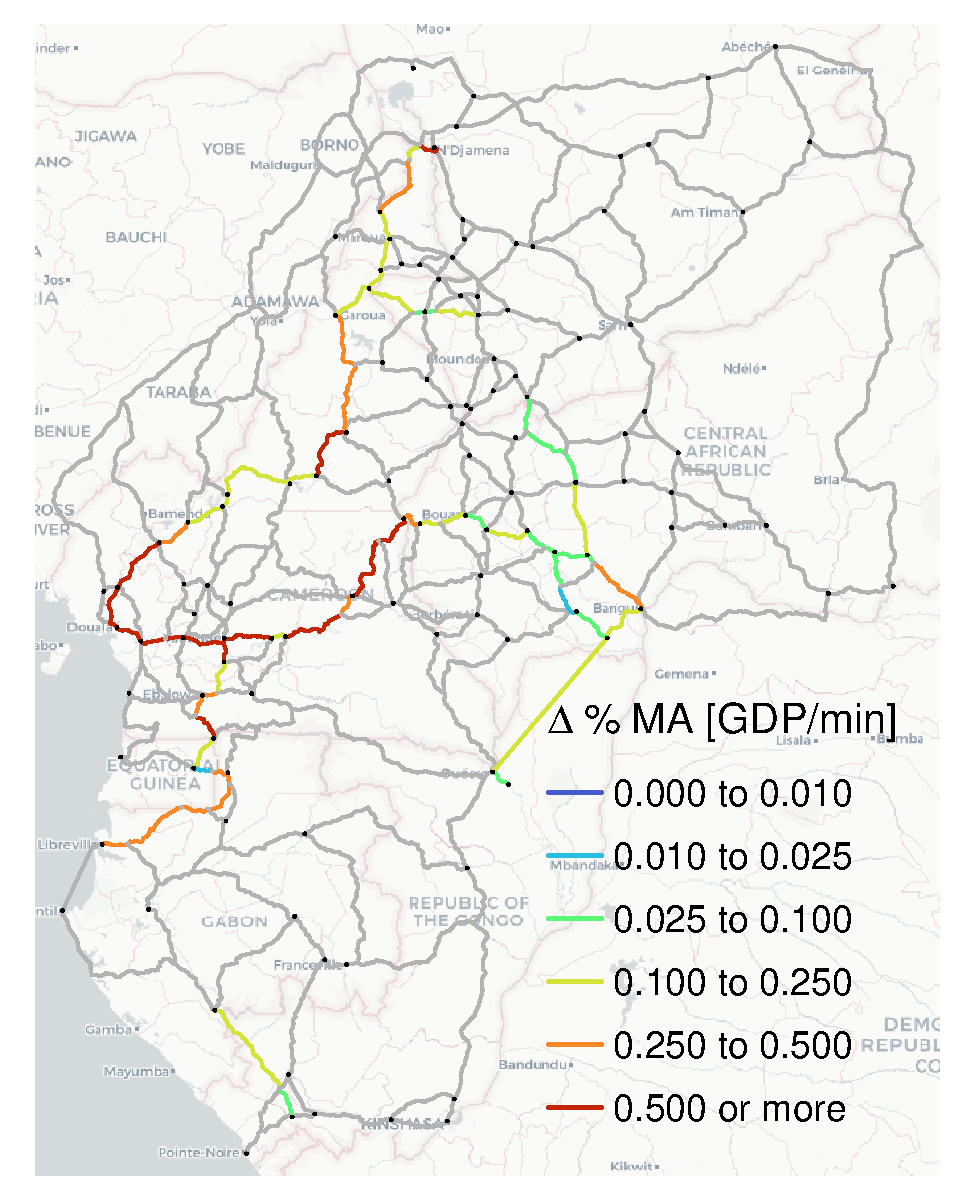
\includegraphics[width=0.48\textwidth]{"../figures/PE/trans_CEMAC_network_MA_100_min_speed_perc_planned_projects.pdf"} &
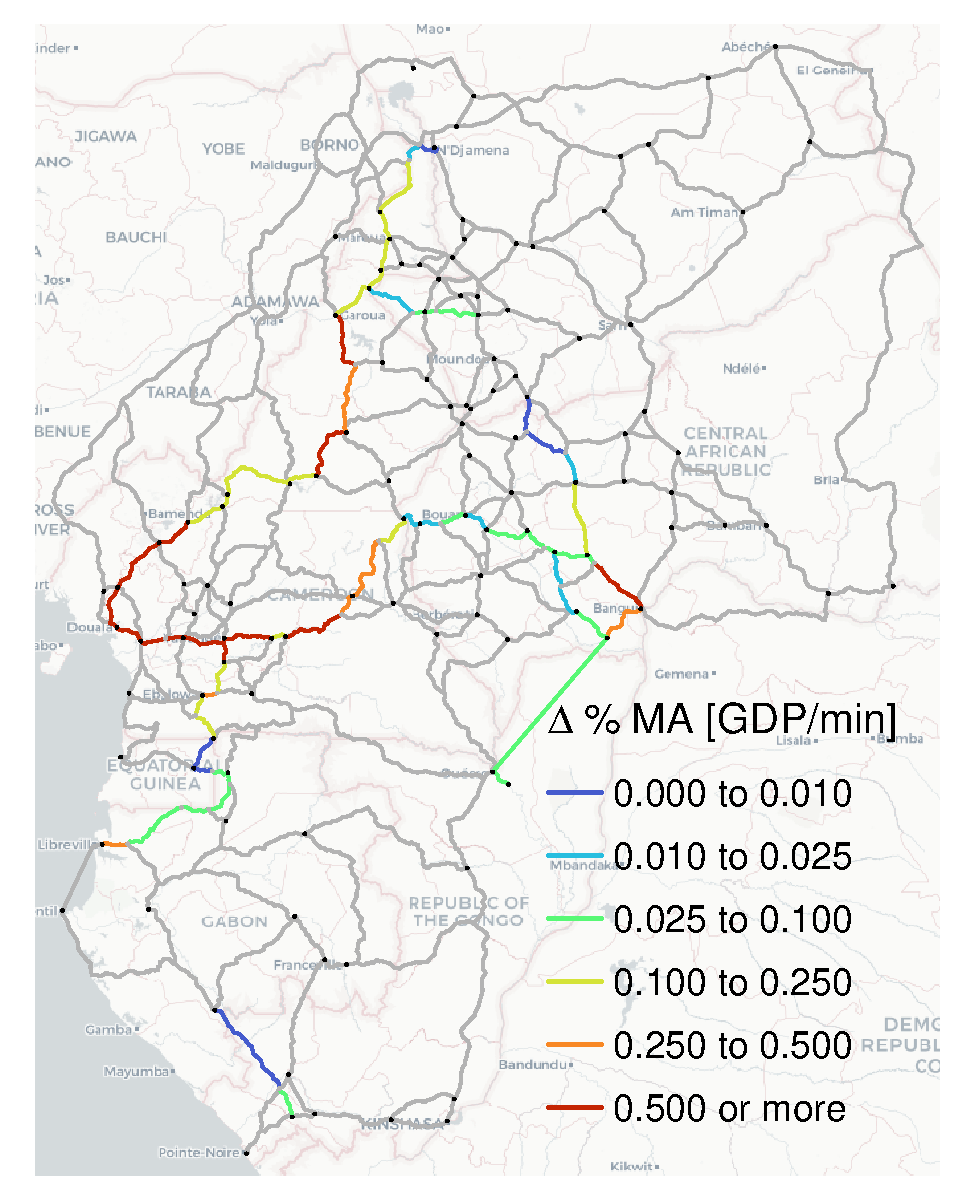
\includegraphics[width=0.48\textwidth]{"../figures/PE/trans_CEMAC_network_MA_100_min_speed_bt_perc_planned_projects.pdf"}  \\ [-0.2em]
\end{tabular}
\raggedright
\scriptsize 
\emph{Notes:} Figure shows total travel-time-denominated MA gains measured (summed) across all trips from upgrading a link to allow travel speeds of $\geq$100km/h for investment projects in the region. 
 % \vspace{-2mm}
\end{figure}

Adding all planned works yields a 1.54\% increase in total MA in the frictionless case. This is significantly larger than the sum of the individual gains which amounts to 0.65\%, indicating that the projects jointly manage to divert more traffic along more optimal routes. The average economic gain is 1.06\$/min/\$, which is not profitable in the short term following \citet{donaldson2016railroads}, but would be profitable in PDV terms if it raises the macroeconomic growth rate by 0.1\% in the 3.5\% baseline growth scenario and by 0.2\% in the 2\% baseline growth scenario.


\begin{figure}[H]  \vspace{-1mm}
\centering
\caption{\label{fig:MA_TT_PUSD} Investment Returns in \$/min/\$ from Building/Upgrading Each Link to $\geq$100km/h}
\vspace{2mm}
\begin{tabular}{cc}
No Frictions & 2019 Doing Business Frictions \\
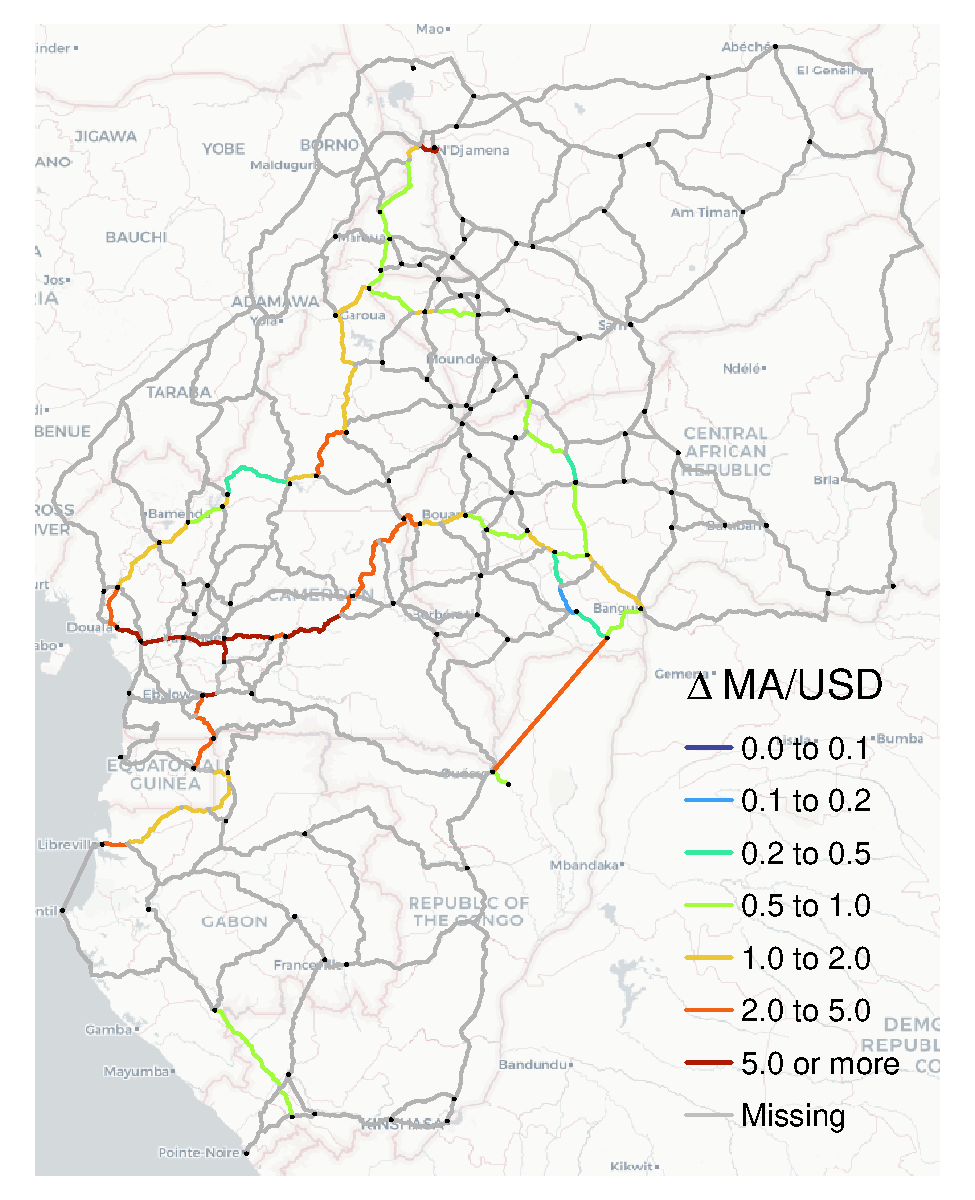
\includegraphics[width=0.48\textwidth]{"../figures/PE/trans_CEMAC_network_MA_gain_all_100kmh_pusd_planned_projects.pdf"} &
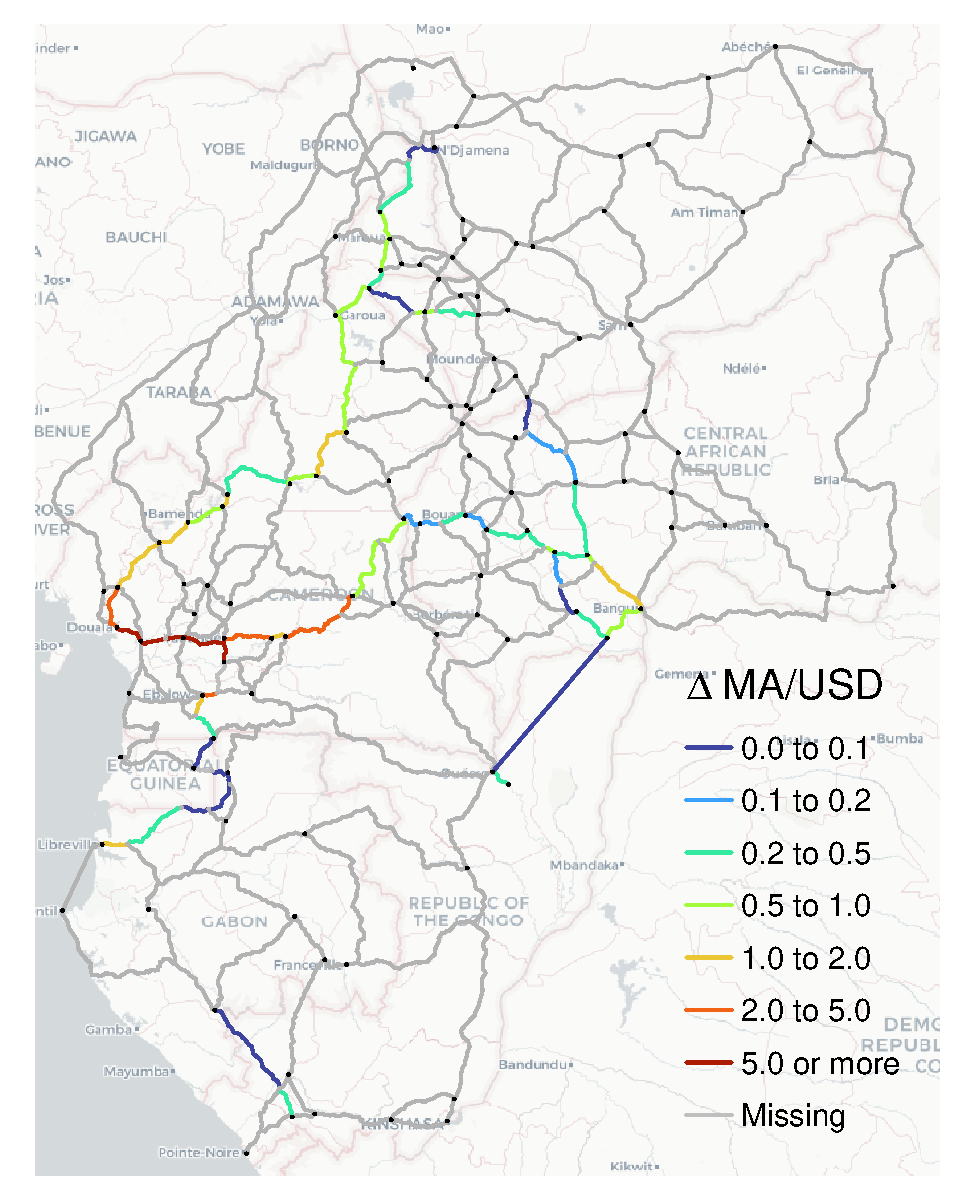
\includegraphics[width=0.48\textwidth]{"../figures/PE/trans_CEMAC_network_MA_gain_all_100kmh_pusd_bt_planned_projects.pdf"}  \\ [-0.2em]
\end{tabular}
\raggedright
\scriptsize 
\emph{Notes:} Figure shows marginal returns in \$/min/\$ (dollar per minute $=$ MA per dollar invested) from upgrading a link to allow travel speeds of $\geq$100km/h or building a new link for road investment projects in the region.
 % \vspace{-2mm}
\end{figure}




% \todo[inline]{To be continued...}


 \newpage


\section{Optimal Network Investments in General Equilibrium}

The General Equilibrium simulations also closely follow \citet{krantz2024optimal}, utilizing the quantitative framework of \citet{fajgelbaum2020optimal} and some parameters taken from \citet{graff2024spatial}. As in \citet{krantz2024optimal}, I let ports produce the imports. Since the region also has land borders, I apply the same scaling factor of 37 to the ports' export volume in 2020 Q1, which is obtained considering imports and ports of the entire continent. This yields that imports through the regions 6 ports are 16.9\% of the regions GDP. The total imports of goods and services in the region from 2019-2023 was 28.2\% of GDP, and the merchandise imports were 19.2\% of GDP, so this assumes that the bulk of merchandise imports came in through the regions 6 international ports.  \newline 

To create incentives for trade through the network, I let 16 cities with a population of $>$200,000 or ports with outflows of $>$1M TEU in 2020 Q1 produce their own product. The remaining cities are classified into port (positive outflows), large city with population $>$ 100,000, medium-sized city with population $>$50,000, and town/unpopulated node otherwise. The nodes are parameterized with IWI productivity and population. Port cities have additional international productivity amounting to $(\text{outflows [TEU] in 2020 Q1}\times 37)/\text{population}$. Edges are parameterized with speed in km/h; infrastructure building cost, iceberg trade cost, and (optionally) border frictions, exactly follow \citet{krantz2024optimal}. Figure \ref{fig:Graph_Calib} shows the classified and parameterized graph. % \newline 

\begin{figure}[H] \vspace{-1mm}
\centering
\caption{\label{fig:Graph_Calib} Calibrated Network for General Equilibrium Simulations}
\vspace{2mm}
\resizebox{\textwidth}{!}{
\begin{tabular}{cc}
Nodes by Type & Calibration Details \\
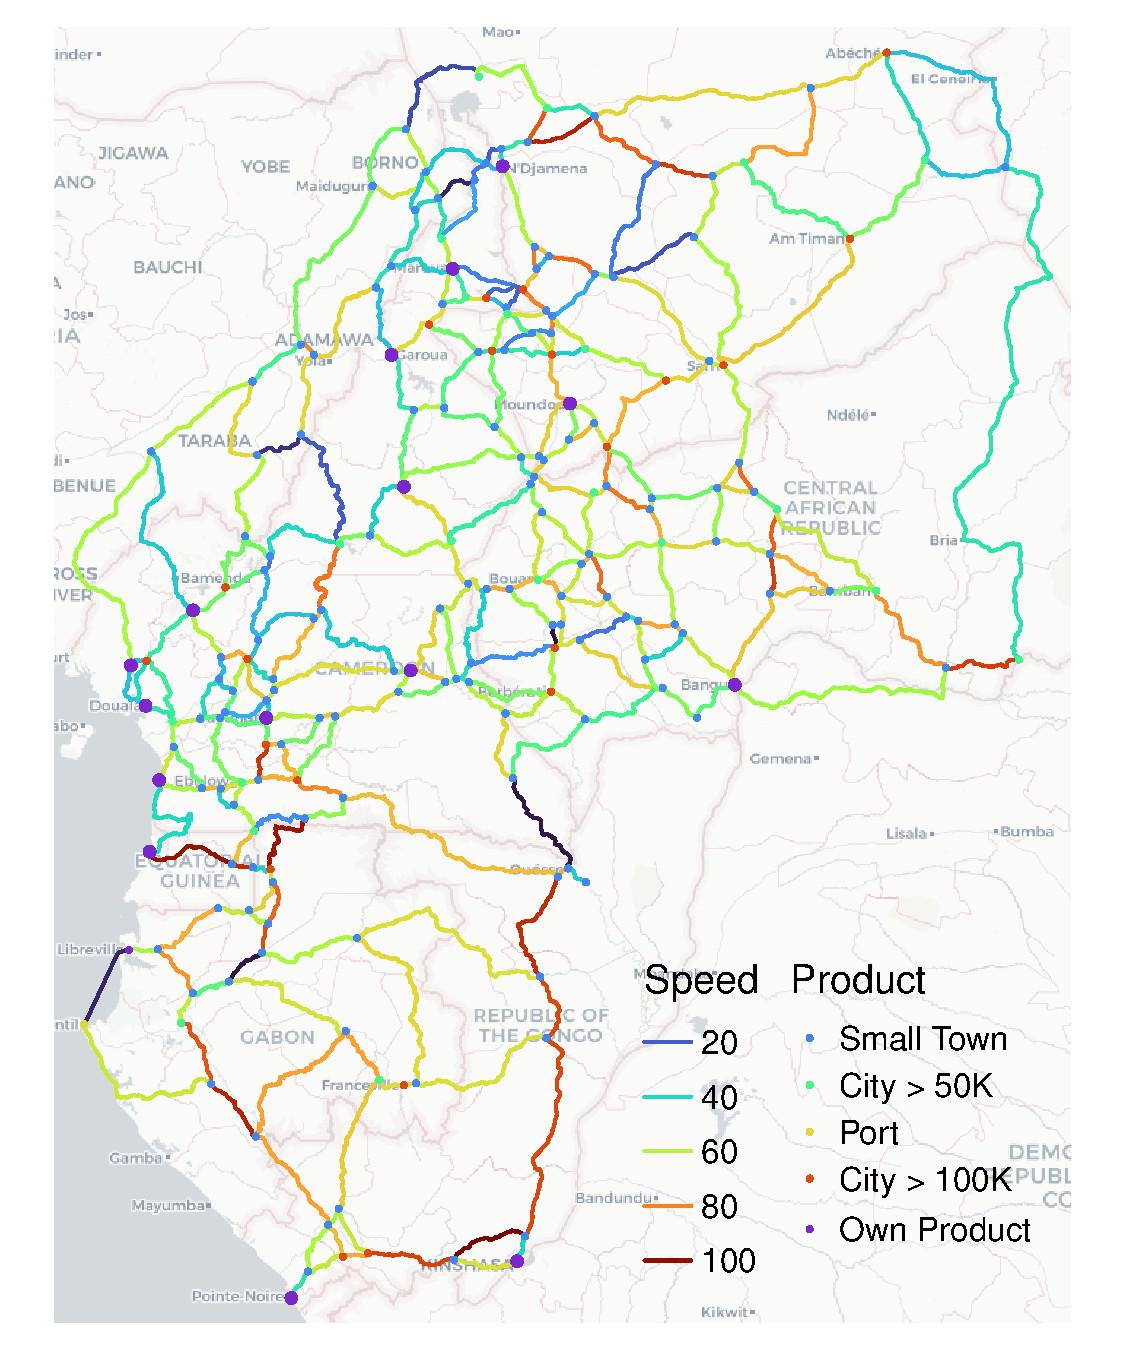
\includegraphics[width=0.505\textwidth]{"../figures/GE/trans_africa_network_reduced_20_products_google.pdf"} &
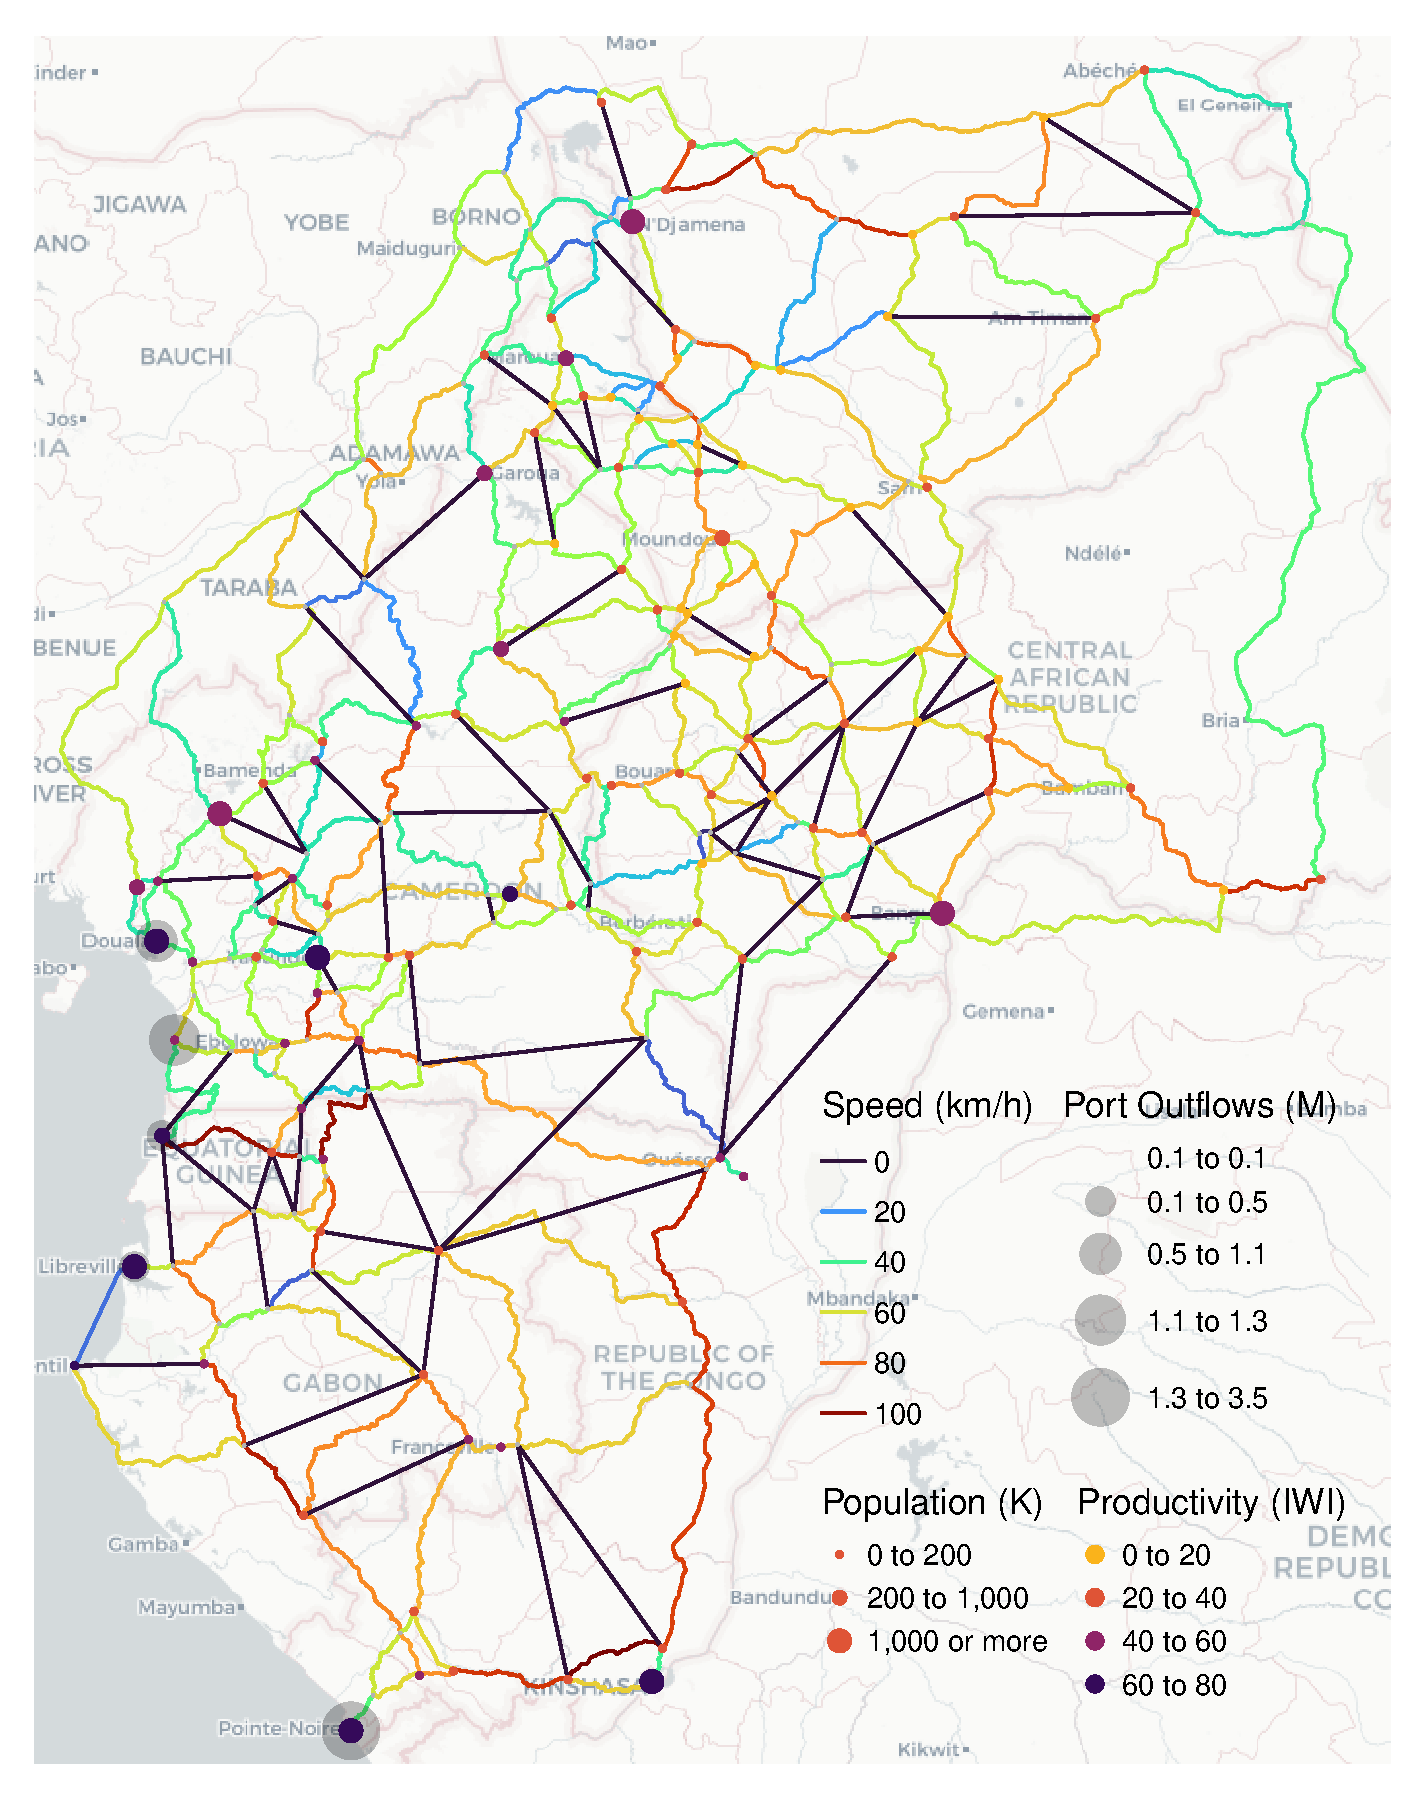
\includegraphics[width=0.48\textwidth]{"../figures/trans_CEMAC_network_GE_parameterization_latest_google.pdf"} \\ [-0.2em]
\end{tabular}
}
% \raggedright
\scriptsize 
\emph{Notes:} Figure shows network calibrated with speed, city population and productivity (IWI) and port outflows. 
% \vspace{-10cm}
\end{figure}

I set the elasticity of substitution equal to $\sigma = 3.8$ following \citet{bajzik2020estimating} and \citet{armington1969theory} because this setting resembles products differentiated by origin traded in an international context. I simulate cases with ($\rho = 2$) or without ($\rho = 0$) inequality aversion and border frictions, as well as with or without new links, for planning budgets of 1 or 2 billion USD'15, which is about 1.19 billion and 2.38 billion in current USD, respectively. The appendix also reports results for a 5 billion budget, which is likely not feasible to summon. As mentioned, upgrading all links to 100km/h would cost 13.5 billion USD'15, and constructing all proposed links would cost 6.1 billion USD'15. I start by reporting results where planners can only upgrade existing roads/connections. 

\subsection{Upgrading Roads} 

Figure \ref{fig:GE_UGNOfr} shows the results, in terms of the fraction of the link upgraded, from planners optimally spending 1 or 2 billion on upgrading the network, without frictions and with or without inequality aversion. Clearly, these planners focus on better connecting the central populated regions, particularly in central Cameroon and at the Cameroon-Chad border area. But also the roads between Point-Noire and Brazzaville and between Bangui and Mbaiki and from Ouesso into Cameroon are upgraded. All planners also upgrade the slow ferry connection between Libreville and 
Port-Gentil, implying that building a road connecting the two has high priority. With inequality aversion, planners spend a bit more in poorer northern Chad and less in the richer coastal regions. % \newline 

% \todo[inline]{Draft, to be continued!}

\begin{figure}[H] \vspace{-1mm}
\centering
\caption{\label{fig:GE_UGNOfr} Welfare Maximizing Infrastructure Spending in GE: Upgrading Links}
\vspace{2mm}
\resizebox{\textwidth}{!}{
\begin{tabular}{cc}
1B Standard Planner & 1B Inequality Averse Planner \\
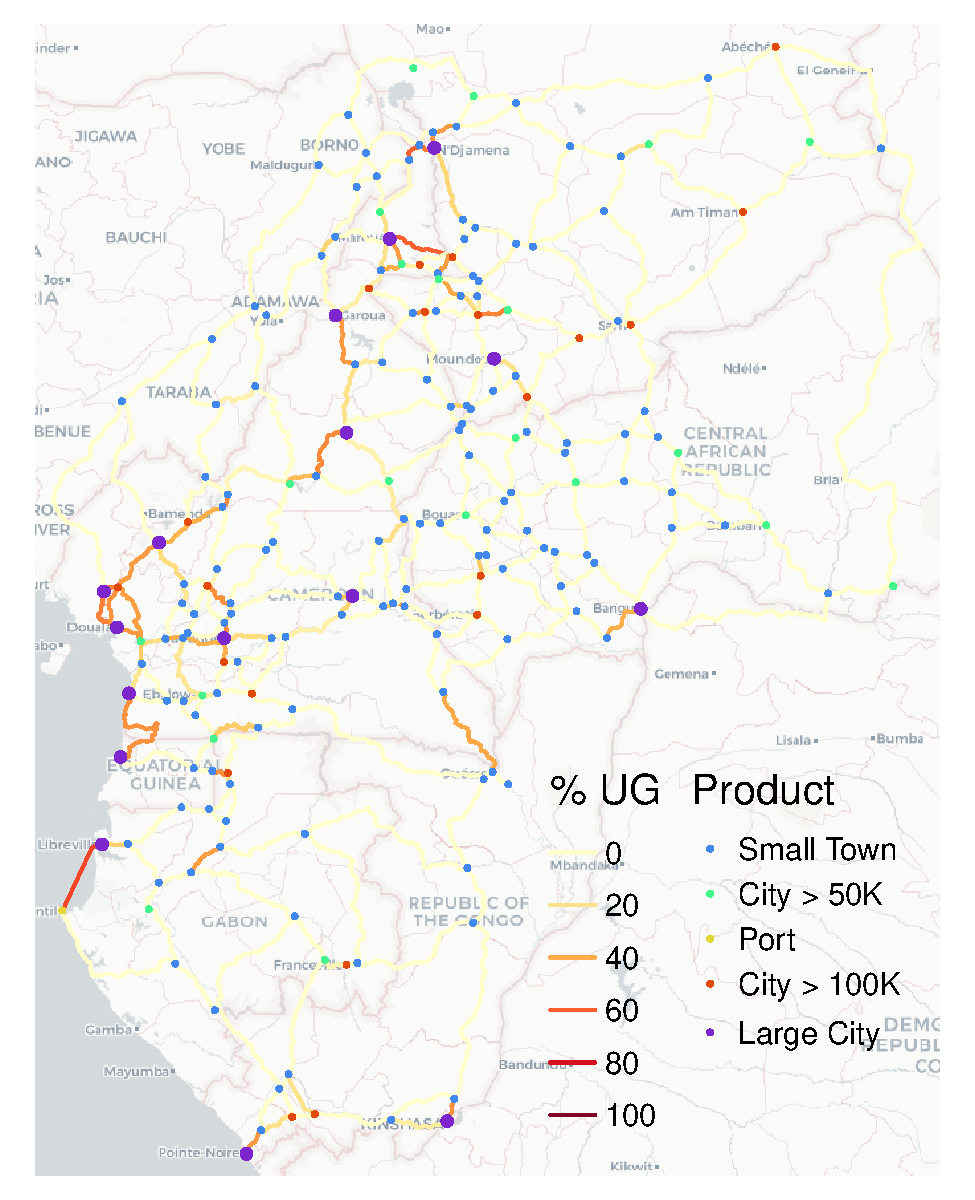
\includegraphics[width=0.48\textwidth]{"../figures/GE/trans_africa_network_GE_20g_1b_fixed_cgc_sigma3.8_rho0_julia_google_perc_ug.pdf"} &
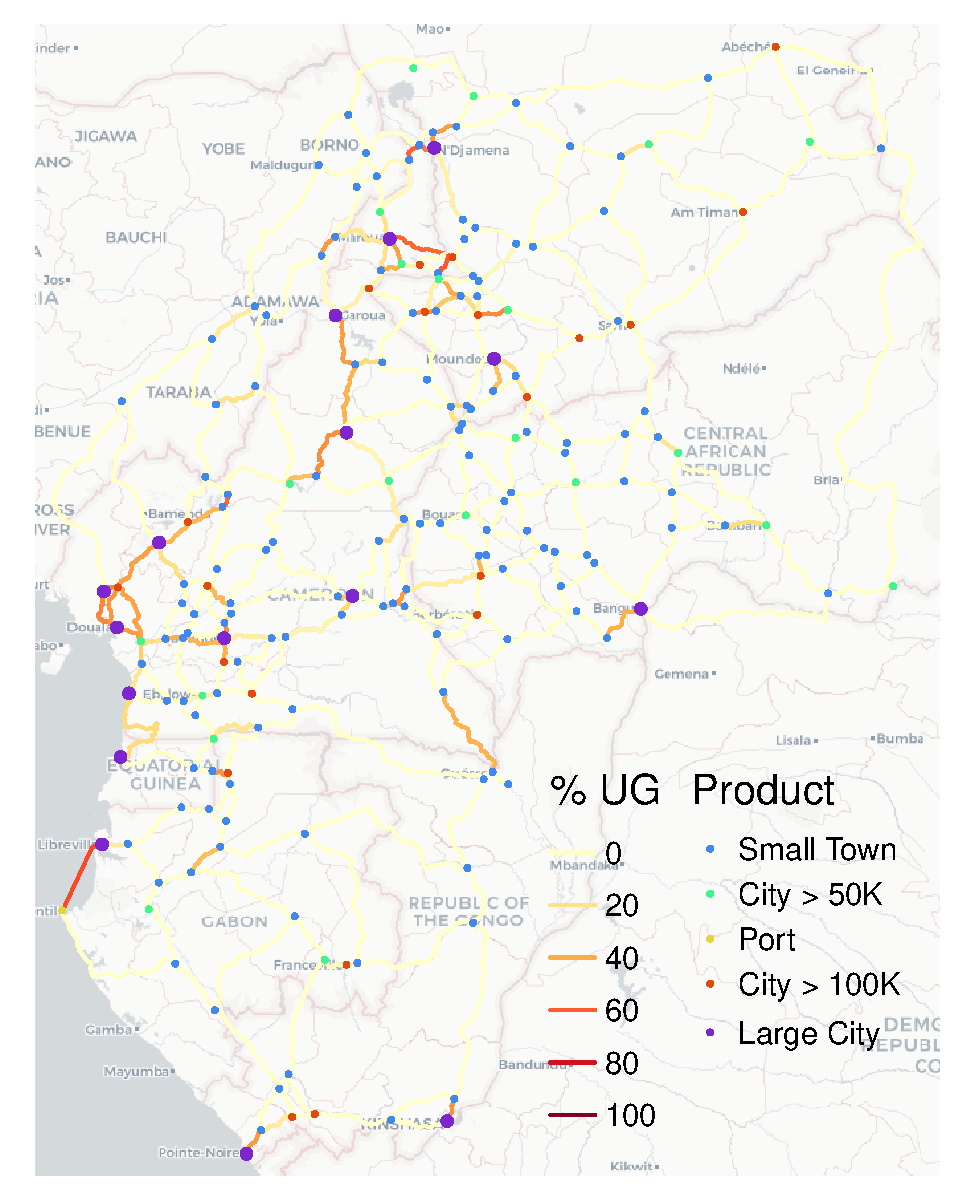
\includegraphics[width=0.48\textwidth]{"../figures/GE/trans_africa_network_GE_20g_1b_fixed_cgc_sigma3.8_rho2_julia_google_perc_ug.pdf"} \\ 
2B Standard Planner & 2B Inequality Averse Planner \\
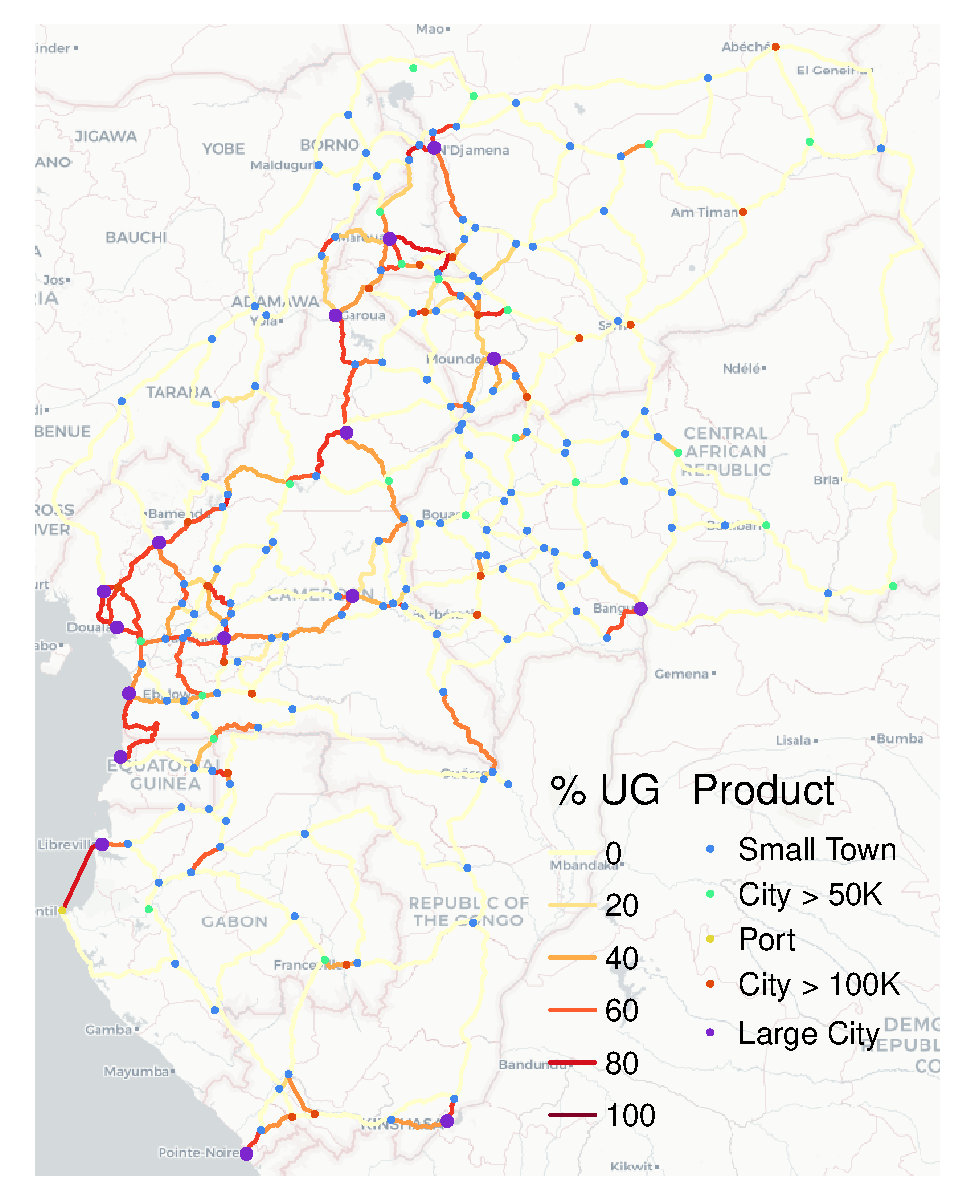
\includegraphics[width=0.48\textwidth]{"../figures/GE/trans_africa_network_GE_20g_2b_fixed_cgc_sigma3.8_rho0_julia_google_perc_ug.pdf"} &
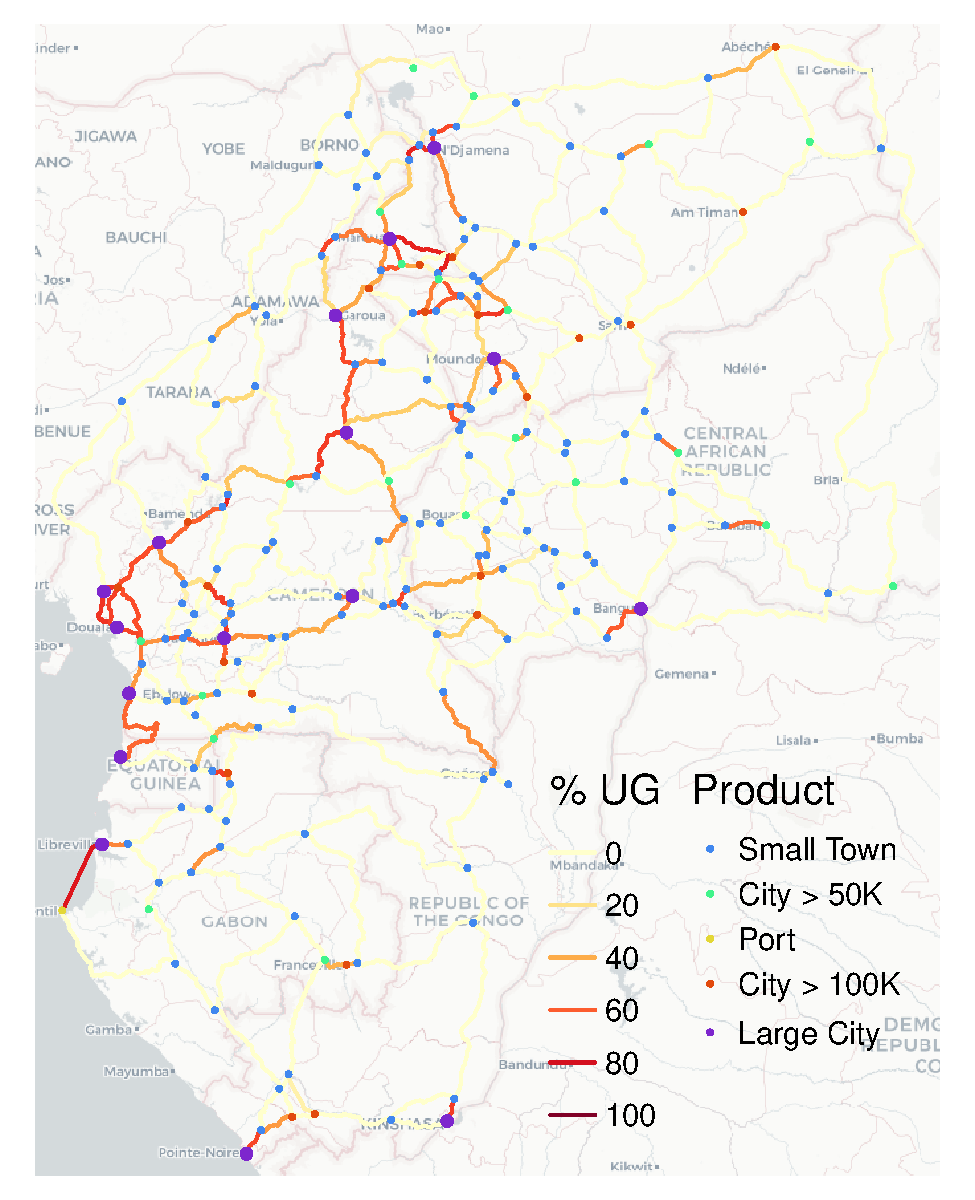
\includegraphics[width=0.48\textwidth]{"../figures/GE/trans_africa_network_GE_20g_2b_fixed_cgc_sigma3.8_rho2_julia_google_perc_ug.pdf"}
\end{tabular}
}
% \raggedright
\scriptsize 
\emph{Notes:} Figure shows the welfare maximizing 1 and 2 billion USD'15 infrastructure spending on upgrading the network without border frictions. Spending is indicated in terms of the \% of each link being upgraded.  
% \vspace{-10cm}
\end{figure}

Appendix Figure \ref{fig:GE_UGNOfr_5b} shows the optimal 5 billion spending. Here the planner upgrades two full corridors from Cameroon up north via Bertoua and Ngaoundere, respectively, and also the full road between Point-Noire and Brazzaville. Under inequality aversion, also the road between Bangui and N'Djamena is updated, alongside many roads connecting cities near the Cameroon-Chad border. \newline  

I also run the simulations with border frictions. Figure \ref{fig:GE_UGFR} reports the difference to the frictionless case. As in \citet{krantz2024optimal}, frictions lead to slight alterations in the optimal allocation away from expensive border-crossing links. In some cases, other border crossing links are strengthened instead, and funds are directed to building more domestic links. Overall, the effects of frictions are small, presumably because they enter iceberg trade costs through a log function (see \citet{krantz2024optimal} Eq. 12), and non-trivial as the resulting reallocations are a complex GE outcome. % \newline 

\begin{figure}[H] \vspace{-1mm}
\centering
\caption{\label{fig:GE_UGFR} Difference in Optimal GE Spending under Frictions: Upgrading Links}
\vspace{2mm}
\resizebox{\textwidth}{!}{
\begin{tabular}{cc}
1B Standard Planner & 1B Inequality Averse Planner \\
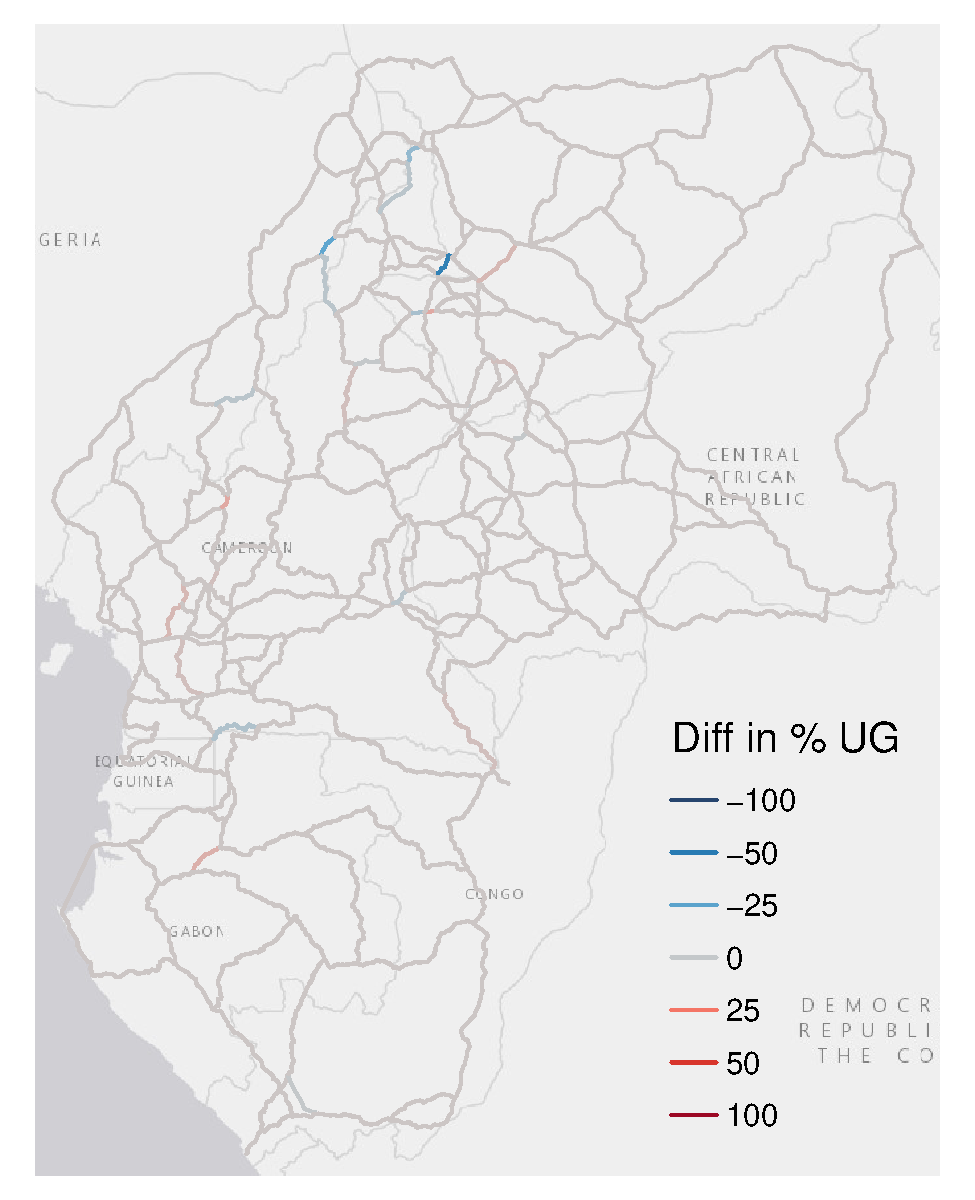
\includegraphics[width=0.48\textwidth]{"../figures/GE/trans_africa_network_GE_20g_1b_fixed_cgc_sigma3.8_rho0_julia_google_Ijk_bc_perc_ug_diff.pdf"} &
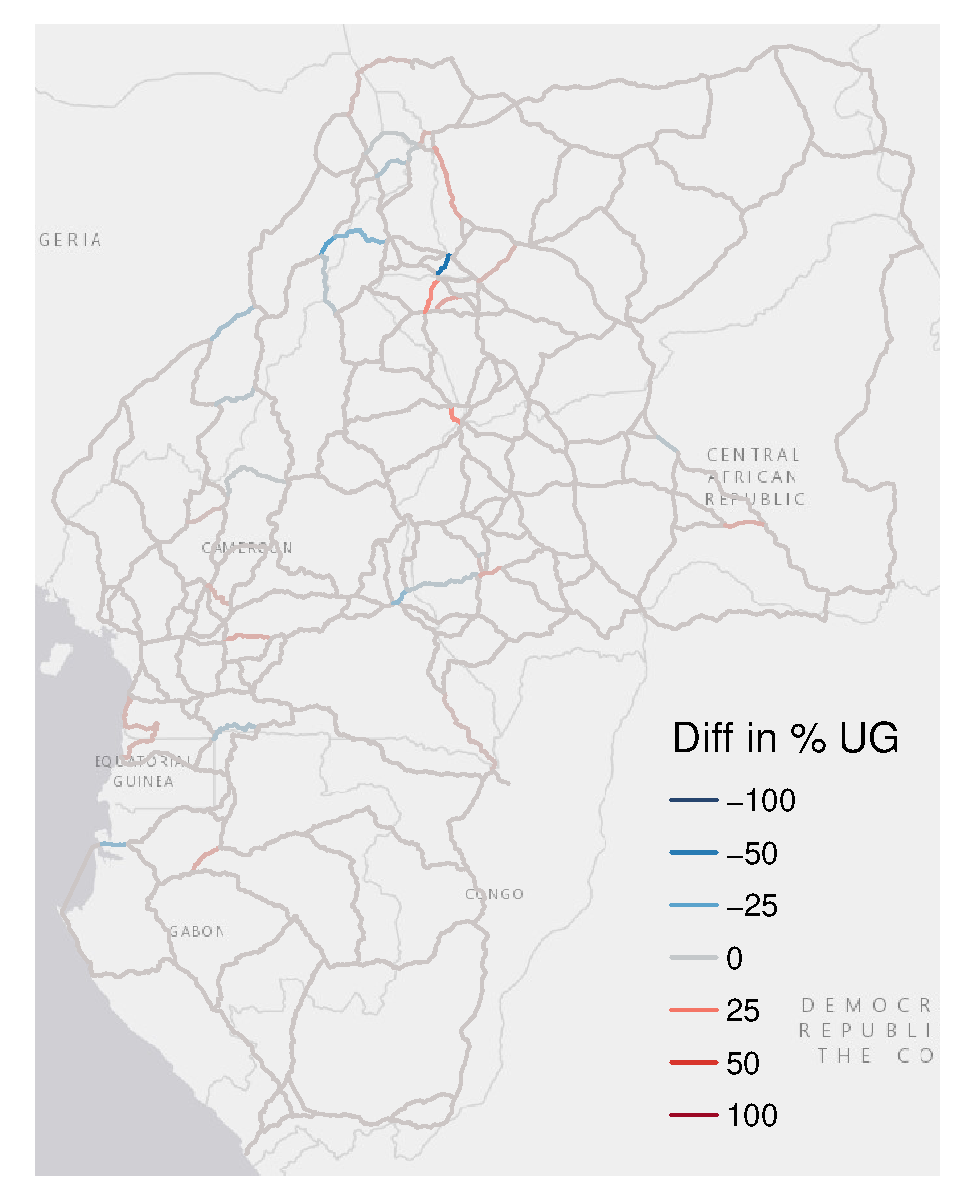
\includegraphics[width=0.48\textwidth]{"../figures/GE/trans_africa_network_GE_20g_1b_fixed_cgc_sigma3.8_rho2_julia_google_Ijk_bc_perc_ug_diff.pdf"} \\ 
2B Standard Planner & 2B Inequality Averse Planner \\
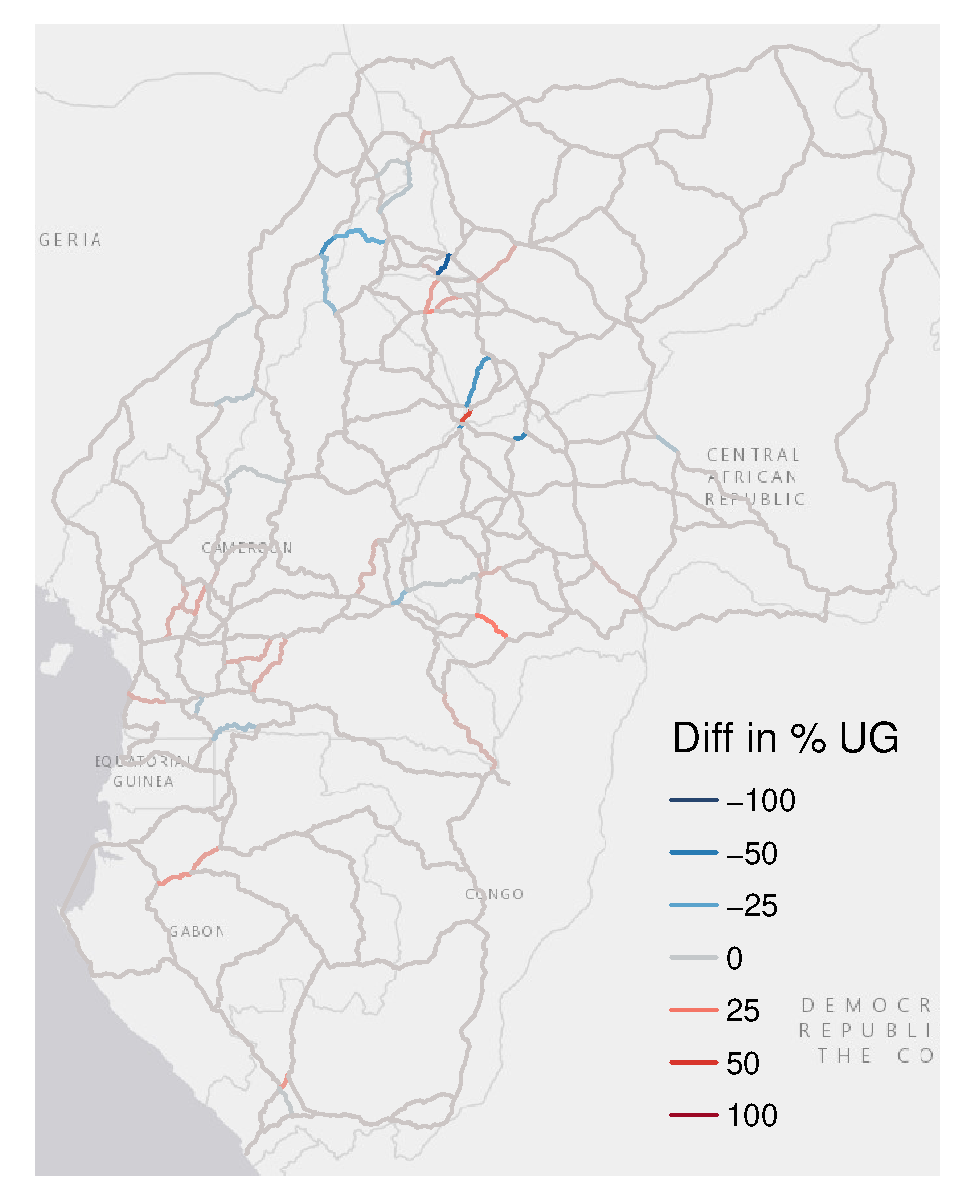
\includegraphics[width=0.48\textwidth]{"../figures/GE/trans_africa_network_GE_20g_2b_fixed_cgc_sigma3.8_rho0_julia_google_Ijk_bc_perc_ug_diff.pdf"} &
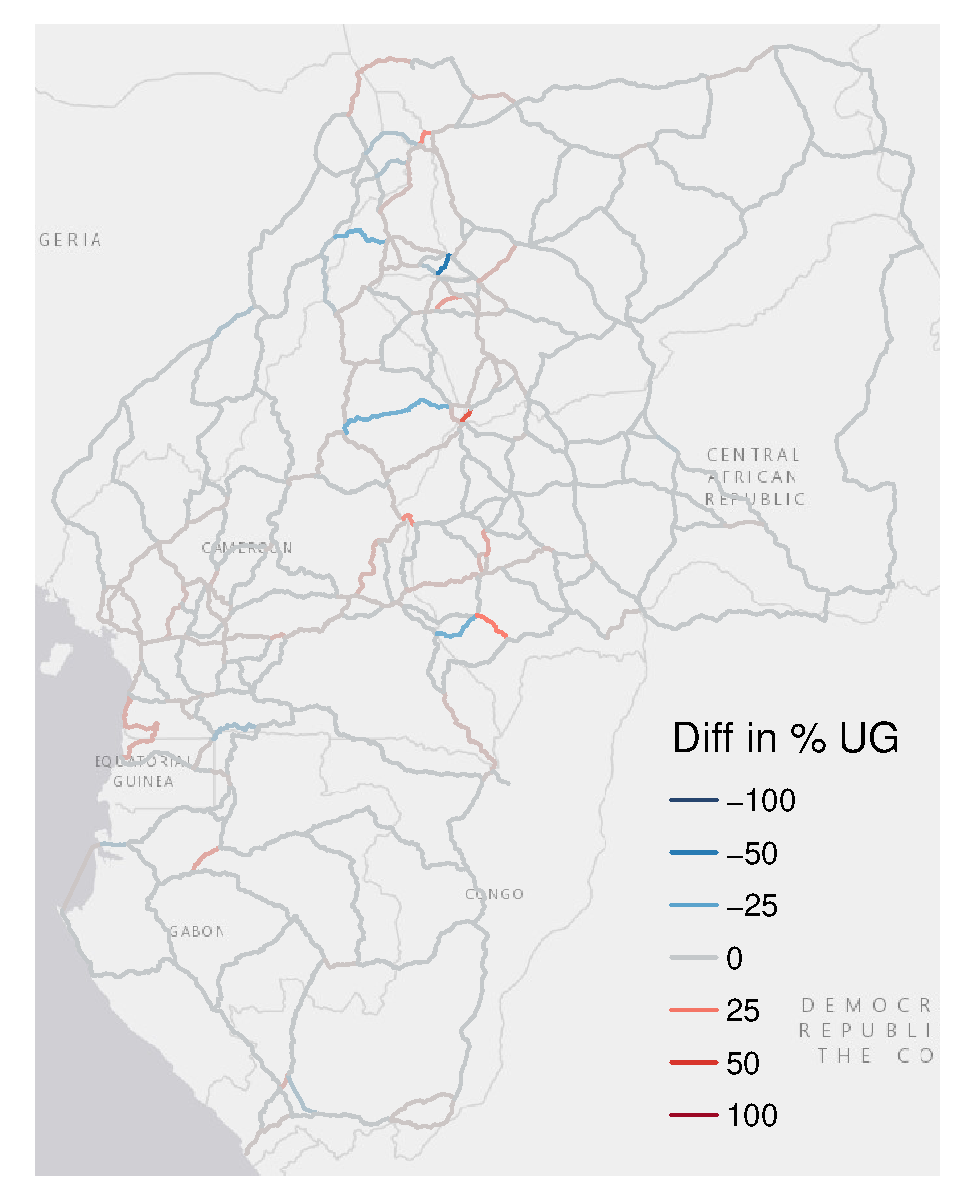
\includegraphics[width=0.48\textwidth]{"../figures/GE/trans_africa_network_GE_20g_2b_fixed_cgc_sigma3.8_rho2_julia_google_Ijk_bc_perc_ug_diff.pdf"}
\end{tabular}
}
% \raggedright
\scriptsize 
\emph{Notes:} Figure shows the difference in optimal spending to the frictionless case. Spending is indicated in terms of the \% of each link being upgraded. Negative (blue) spending is removed under frictions whereas positive (red) is added instead. 
% \vspace{-10cm}
\end{figure}

With 5 billion USD'15 budget shown in Appendix Figure \ref{fig:GE_UGNOfr_5b}, frictions have a more substantial impacts reducing cross-border spending, especially across the Cameroon-Chad border and Cameroon-CAR borders, but also at the border to Equatorial Guinea. 

% \todo[inline]{To be continued...}

\subsection{Building and Upgrading Roads} 

When planners also have the ability to build new roads alongside upgrading existing ones, they almost exclusively choose to do so, despite such links being more expensive. This stands in contrast to results for the entire African network \citep{krantz2024optimal}, indicating that particularly in the CEMAC region much could also be gained by constructing new road segments. Figure \ref{fig:GE_BUGNOfr} shows the results for the standard planner. I was not able to solve the model for the inequality averse planner, where the utility function is more complex. Under frictions, shown in the bottom panel of Figure \ref{fig:GE_BUGNOfr}, investments in certain border-crossing links are again reduced in favour of others and domestic links. Again this is a complex equilibrium outcome. Appendix Figure \ref{fig:GE_UG_5b} shows the 5B planner's allocation, which involves some upgrades but still confirms that many new roads should be built. 

\begin{figure}[H] \vspace{-1mm}
\centering
\caption{\label{fig:GE_BUGNOfr} Welfare Maximizing Infrastructure Spending in GE: Building \& Upgrading Links}
\vspace{2mm}
\resizebox{\textwidth}{!}{
\begin{tabular}{cc}
1B Standard Planner & 2B Standard Planner \\
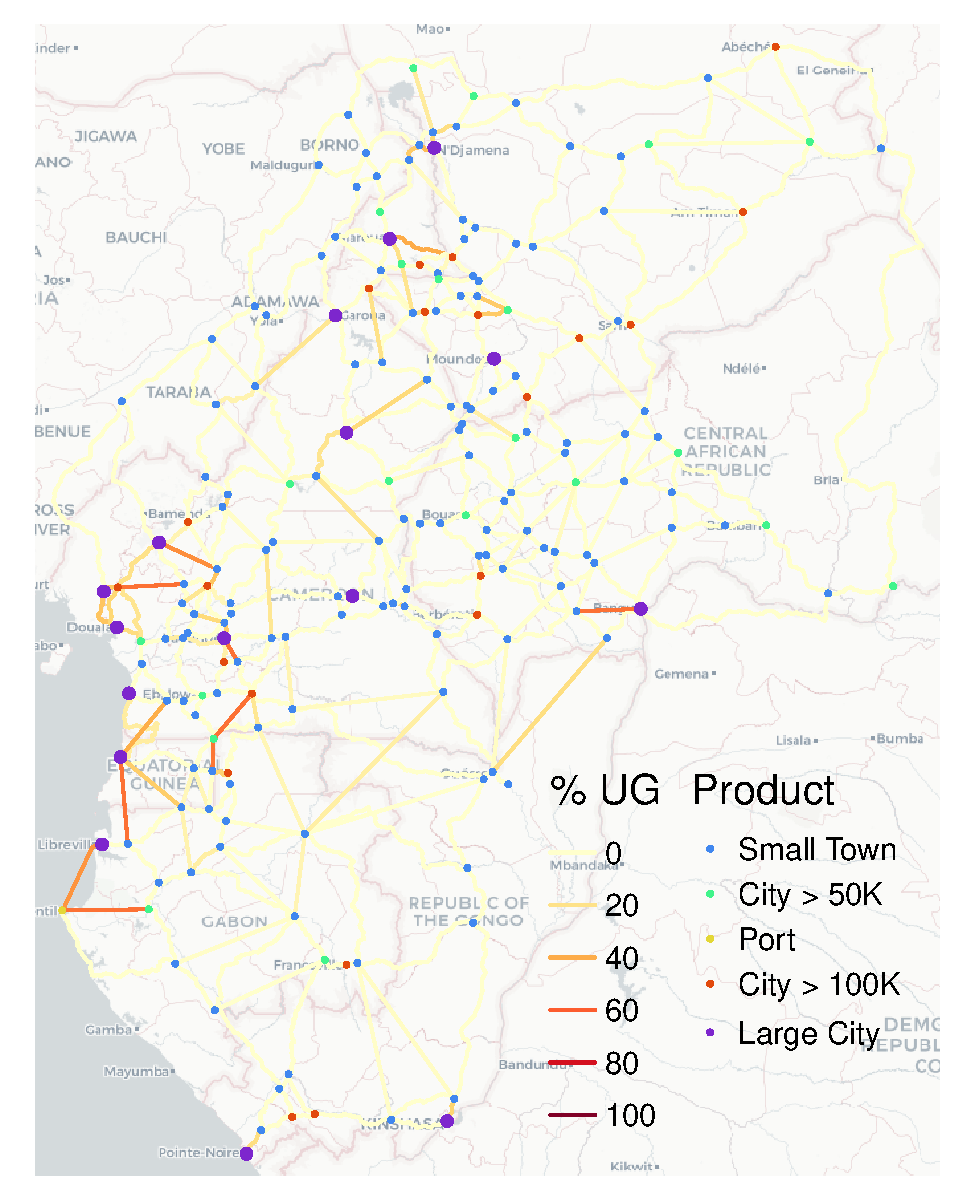
\includegraphics[width=0.48\textwidth]{"../figures/GE/trans_africa_network_GE_add_20g_1b_fixed_cgc_sigma3.8_rho0_julia_google_perc_ug.pdf"} &
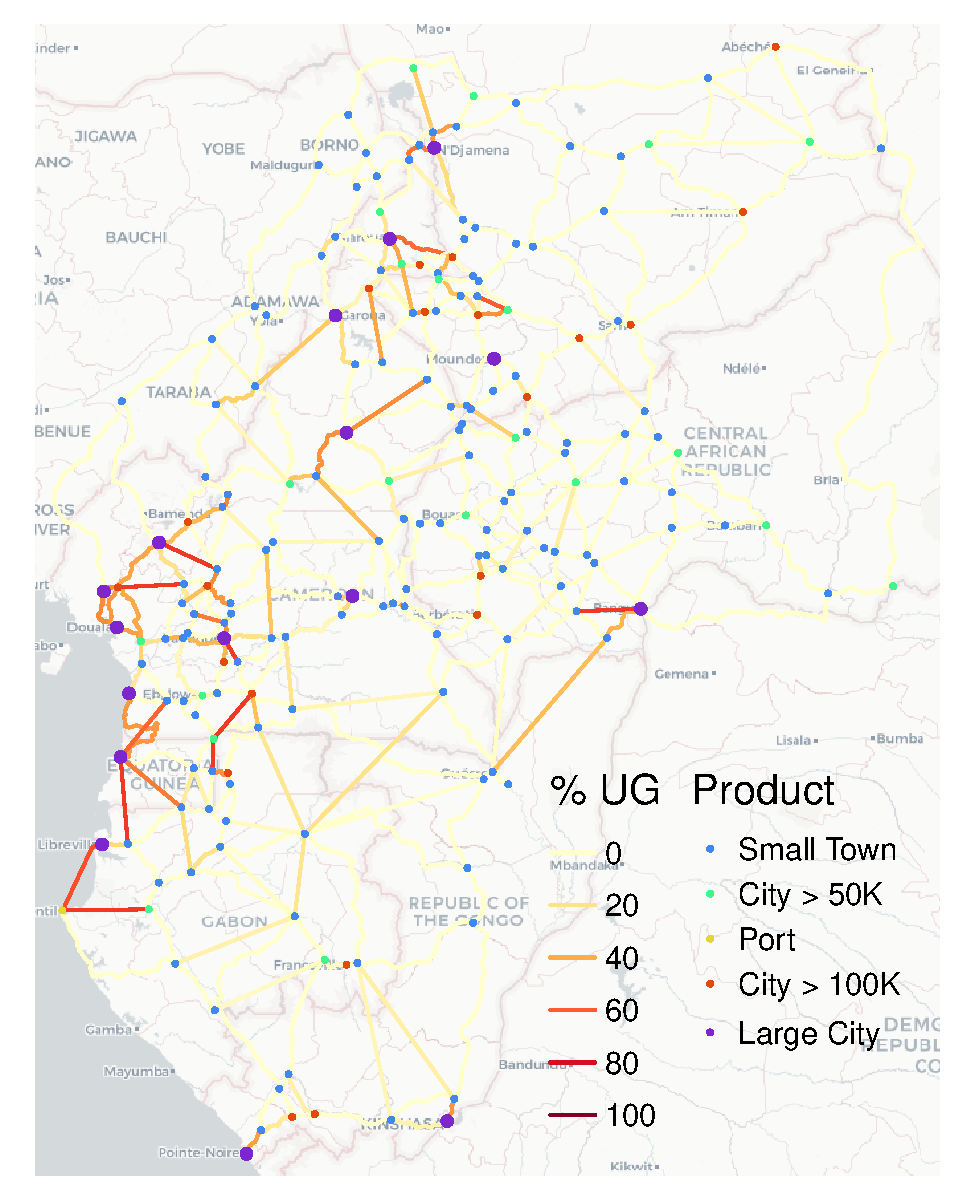
\includegraphics[width=0.48\textwidth]{"../figures/GE/trans_africa_network_GE_add_20g_2b_fixed_cgc_sigma3.8_rho0_julia_google_perc_ug.pdf"} \\ 
1B Standard Planner: Frictions & 2B Standard Planner: Frictions \\
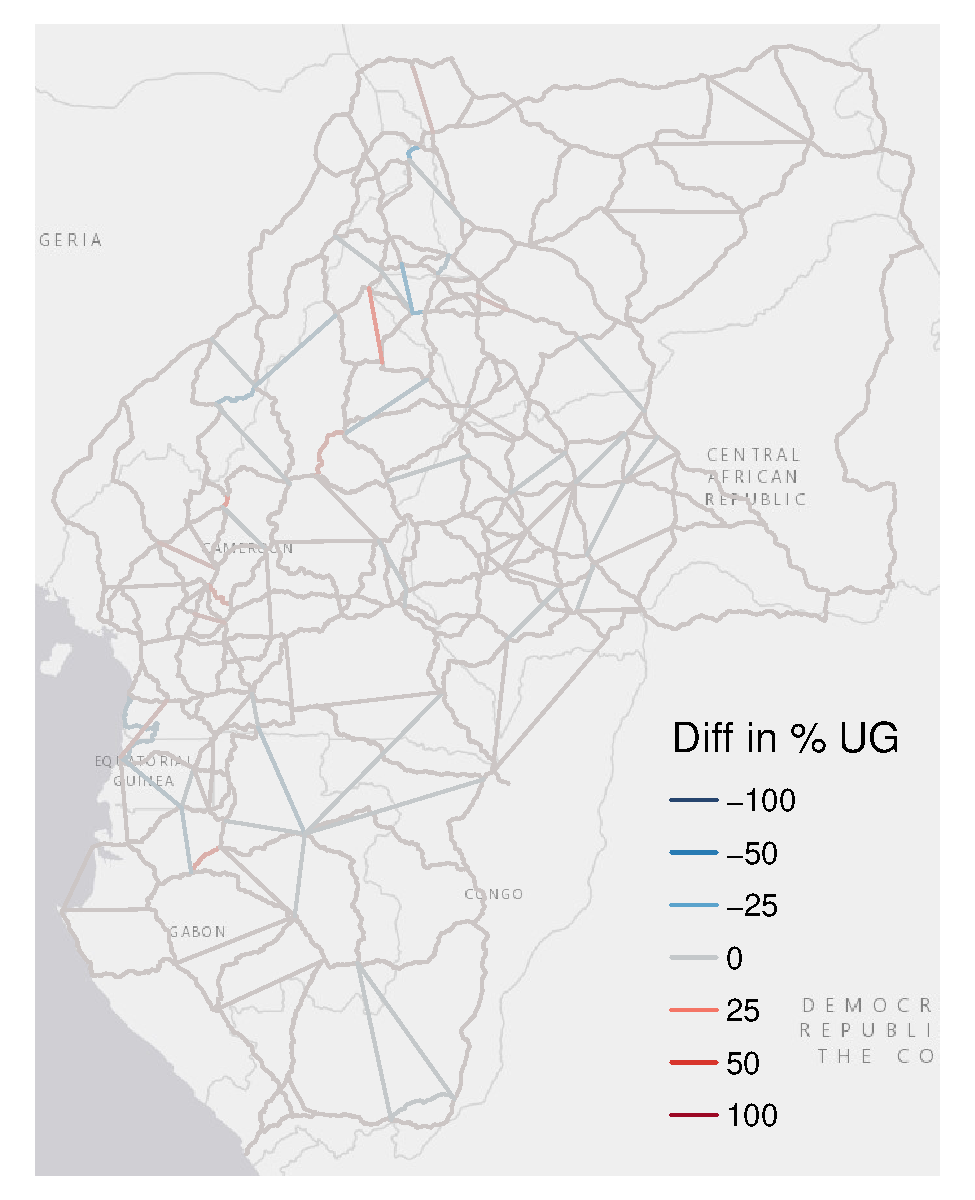
\includegraphics[width=0.48\textwidth]{"../figures/GE/trans_africa_network_GE_add_20g_1b_fixed_cgc_sigma3.8_rho0_julia_google_Ijk_bc_perc_ug_diff.pdf"} &
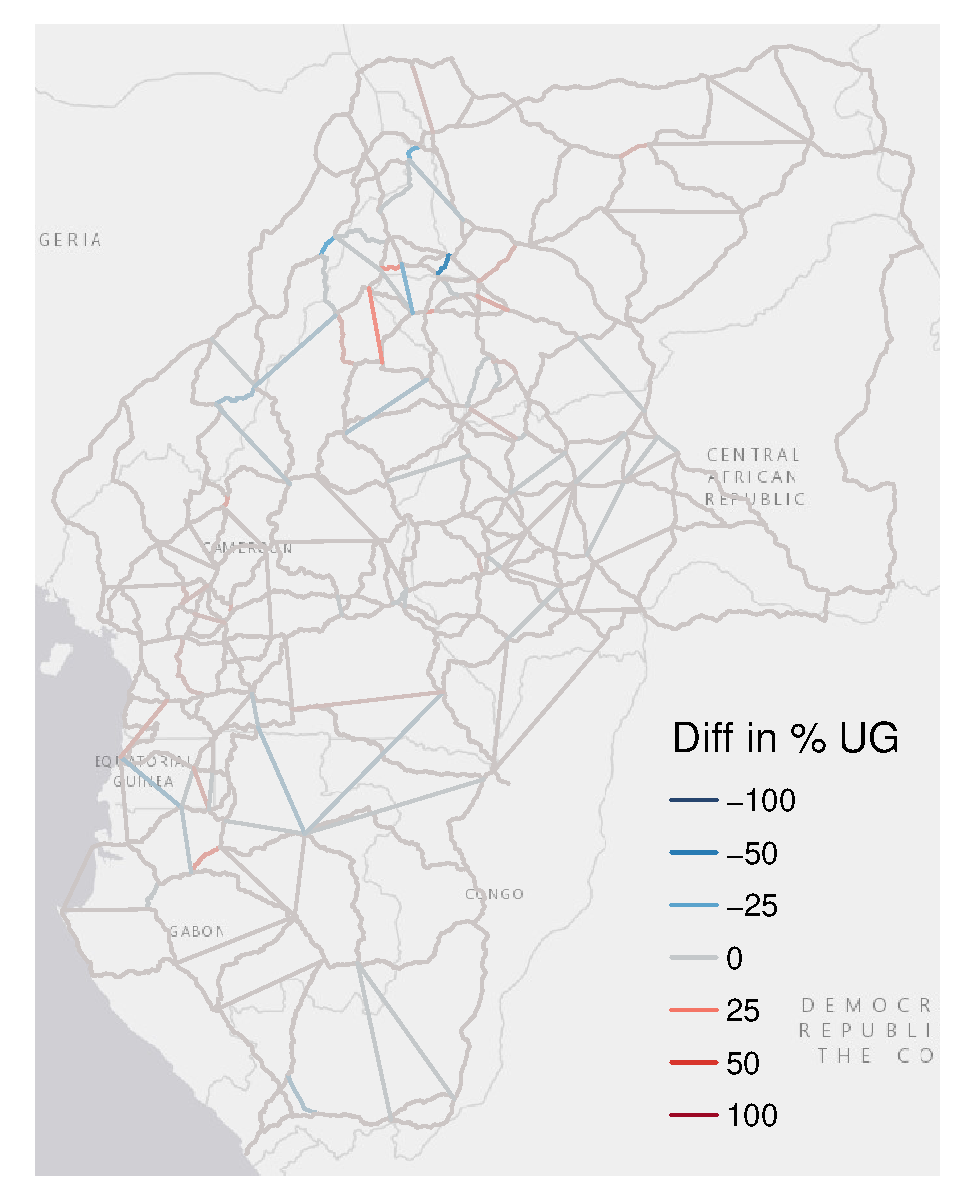
\includegraphics[width=0.48\textwidth]{"../figures/GE/trans_africa_network_GE_add_20g_2b_fixed_cgc_sigma3.8_rho0_julia_google_Ijk_bc_perc_ug_diff.pdf"}
\end{tabular}
}
\raggedright
\scriptsize 
\emph{Notes:} Figure shows the welfare maximizing 1 and 2 billion USD'15 infrastructure spending on building and upgrading the network. Spending is indicated in terms of the \% of each link being upgraded. The bottom panel shows the difference in spending under frictions: Negative (blue) spending is removed under frictions whereas positive (red) is added instead. Inequality averse planners are not reported due to difficulties solving the model in this case. \\ \vspace{-1cm}
\end{figure}

\hphantom{a}
\newpage

\section{Conclusion} 

Analyzing the road network of the CEMAC region and optimal investments into it following the methodology of \citet{krantz2024optimal} yields rich and detailed insights into local and regional investment potentials in partial and general equilibrium. The first general insight is that borders in the region are thick and frictions should duly be reduced. This alone could increase travel time denominated market access (MA) by 77\% and distance-denominated MA by 43\%. Many links are slow at a median speed of 60km/h and need upgrading. Upgrading roads near populated areas in Cameroon (Douala and Yaounde), as well as Brazzaville, Point-Noire, Bangui and N'Djamena, yields high MA and welfare gains relative to the costs. Much can also be gained from building new links that increase route efficiency. Particularly to mention here is better connecting Equatorial Guinea (Bata) to the north (Kiribi) and south (Libreville), and Libreville to Port-Gentil in Gabon. Planned road projects in the regions such as CD13 manage to shift some traffic to the East around Bangui, and are jointly more effective than individually. They are, however, mostly in remote areas and thus not market access or welfare maximizing. Their short-term economic returns may thus be called into question. High-yield upgrading packages around the aforementioned urban centers on the other hand yield sizeable economic returns in both the short and medium run that are likely to outweigh project costs.  % in light of what could be gained by better connecting populated areas. 


\newpage

\bibliographystyle{apacite}
\bibliography{bibliography} % This links to a file bibliography.bib with the citations

\newpage
\section*{Appendix}

\begin{figure}[H] \vspace{-1mm}
\centering
\caption{\label{fig:ACLED} ACLED Armed Conflict Events 2018-2014} 
\vspace{2mm}
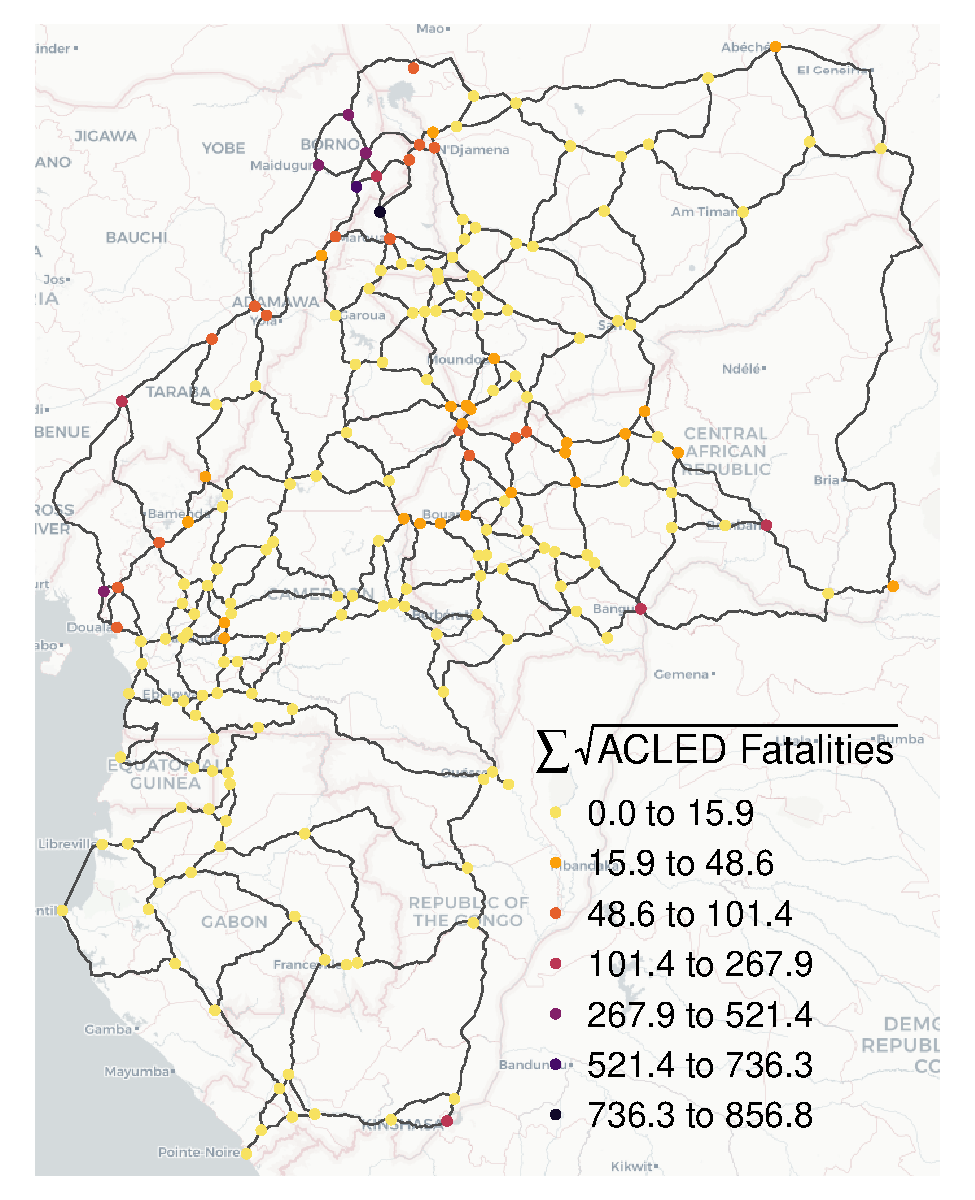
\includegraphics[width=0.9\textwidth]{"../figures/trans_CEMAC_network_ACLED.pdf"} \\
% \raggedright
\scriptsize 
\emph{Notes:} Figure shows ACLED \citep{raleigh2023political} armed conflict events between 2018 and 2024.
% \vspace{-2mm}
\end{figure}

\begin{figure}[h!] \vspace{-2mm}
\centering
\caption{\label{fig:GE_UGNOfr_5b} Welfare Maximizing Infrastructure Spending in GE: Upgrading Links (5B)}
\vspace{2mm}
\resizebox{\textwidth}{!}{
\begin{tabular}{cc}
5B Standard Planner & 5B Inequality Averse Planner \\
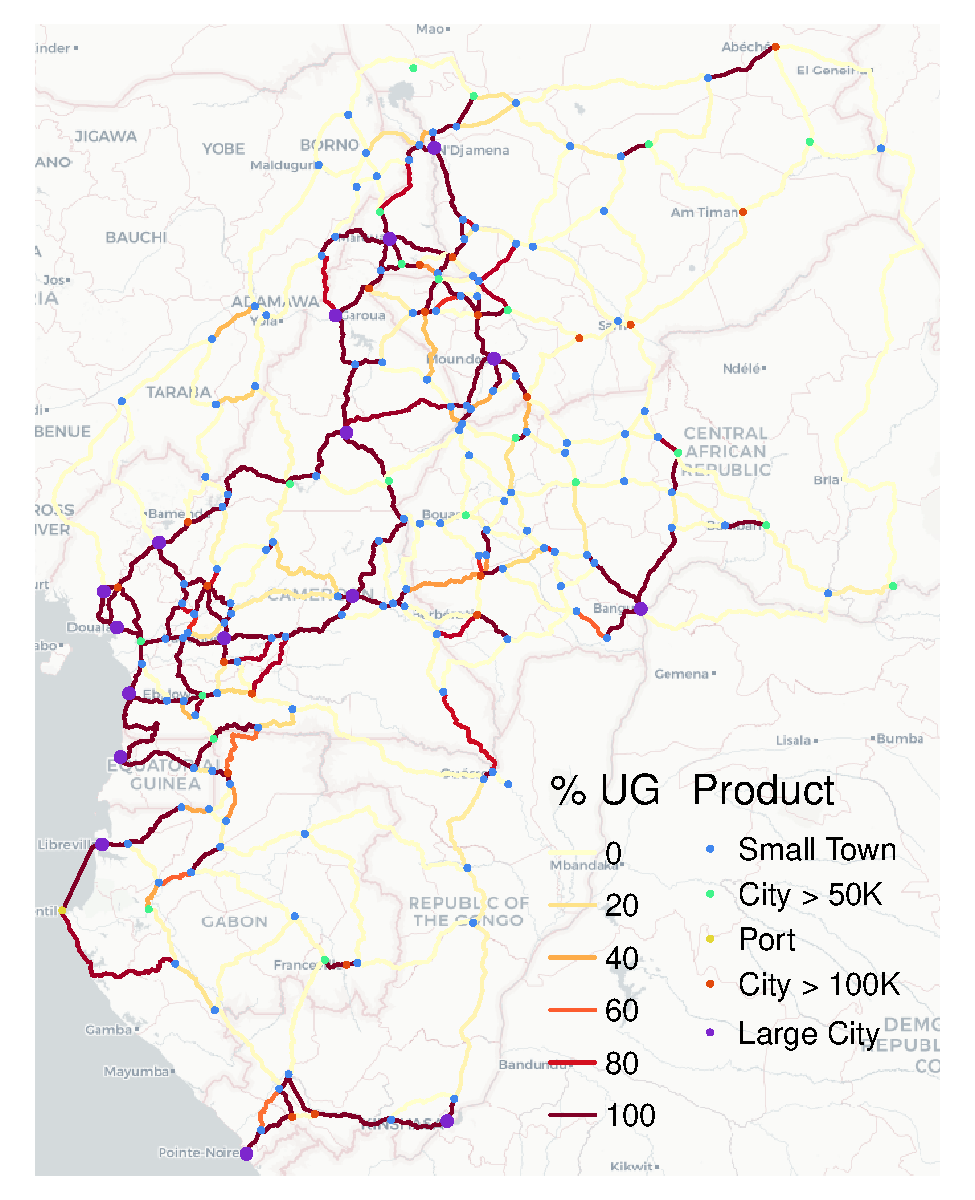
\includegraphics[width=0.48\textwidth]{"../figures/GE/trans_africa_network_GE_20g_5b_fixed_cgc_sigma3.8_rho0_julia_google_perc_ug.pdf"} &
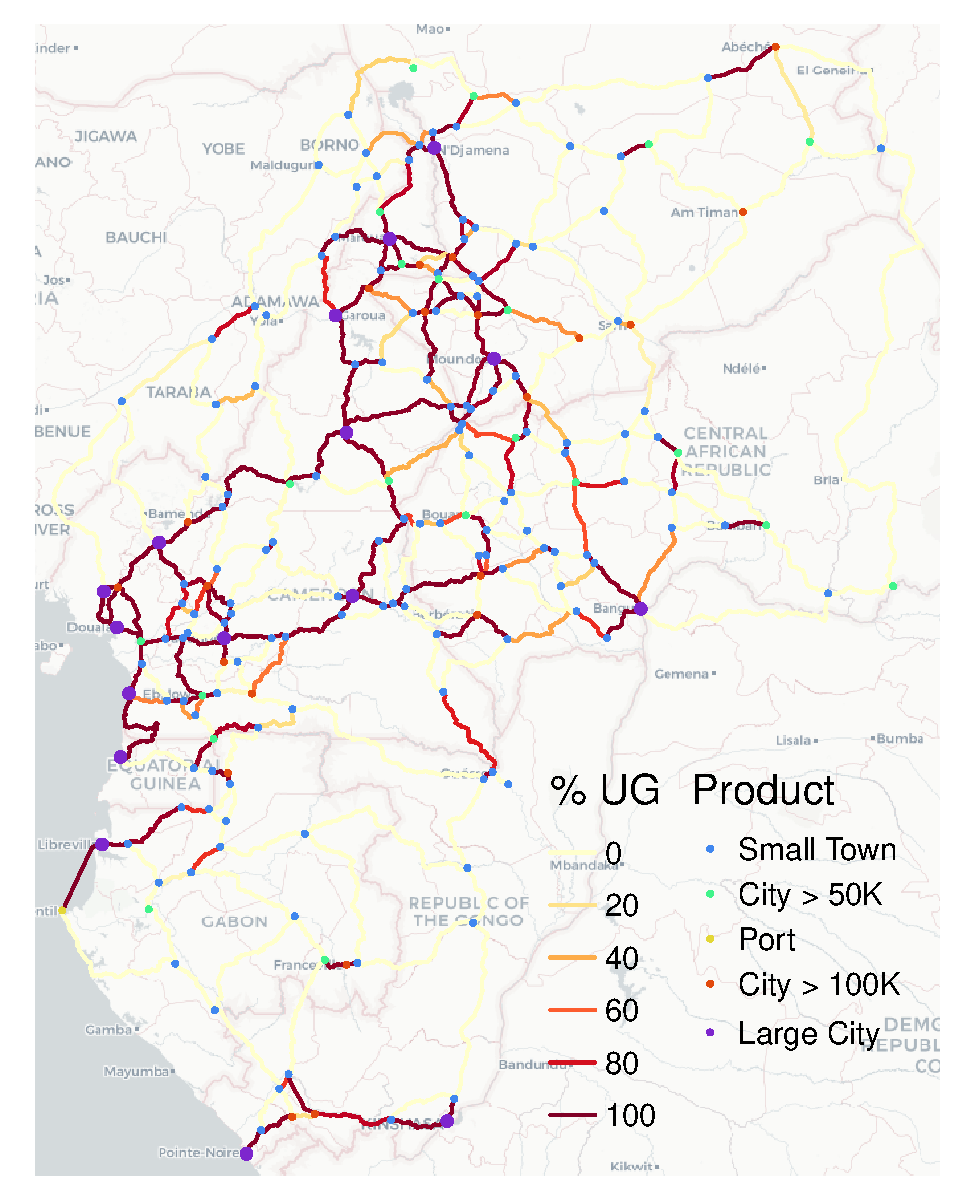
\includegraphics[width=0.48\textwidth]{"../figures/GE/trans_africa_network_GE_20g_5b_fixed_cgc_sigma3.8_rho2_julia_google_perc_ug.pdf"} \\
5B Standard Planner: Frictions & 5B Inequality Averse Planner: Frictions \\
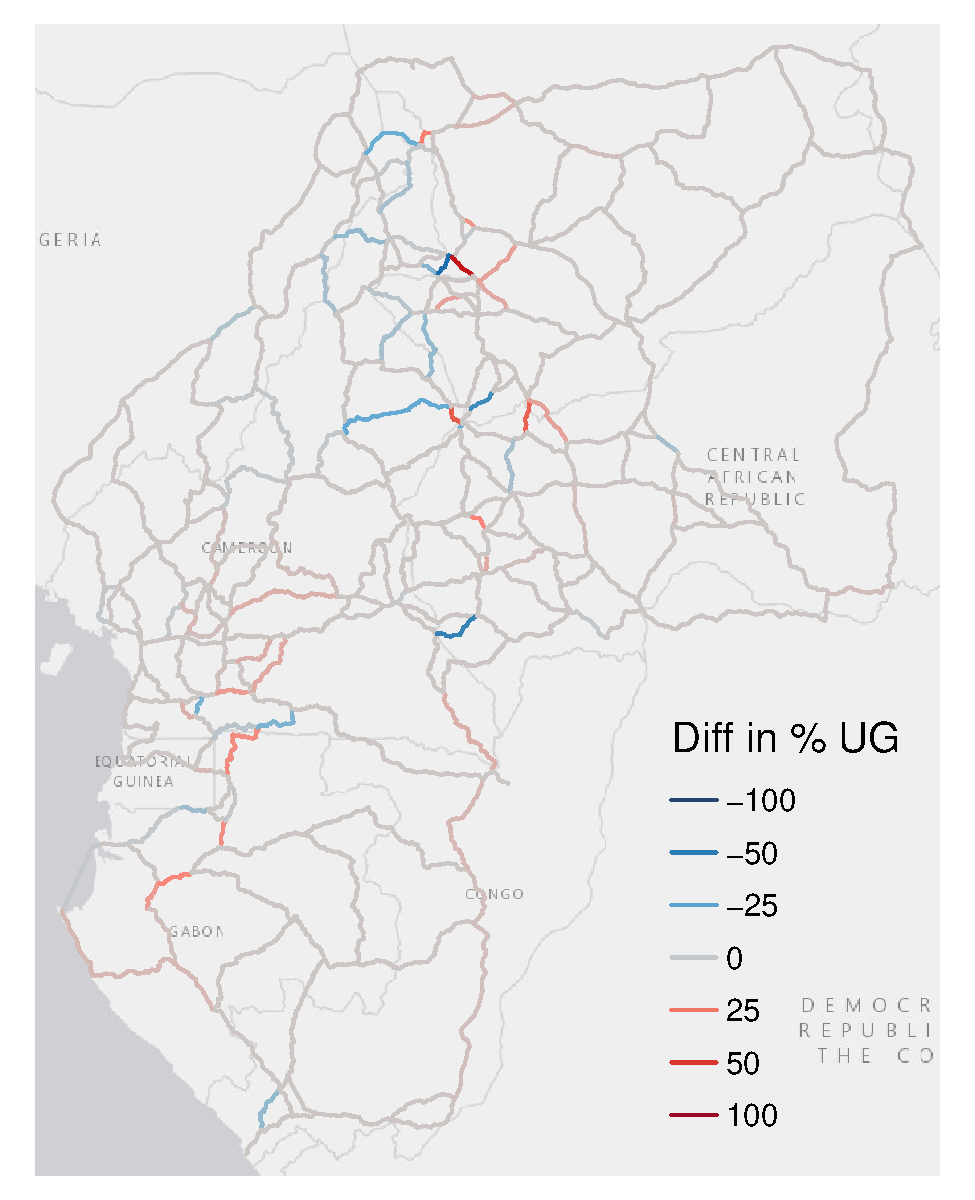
\includegraphics[width=0.48\textwidth]{"../figures/GE/trans_africa_network_GE_20g_5b_fixed_cgc_sigma3.8_rho0_julia_google_Ijk_bc_perc_ug_diff.pdf"} &
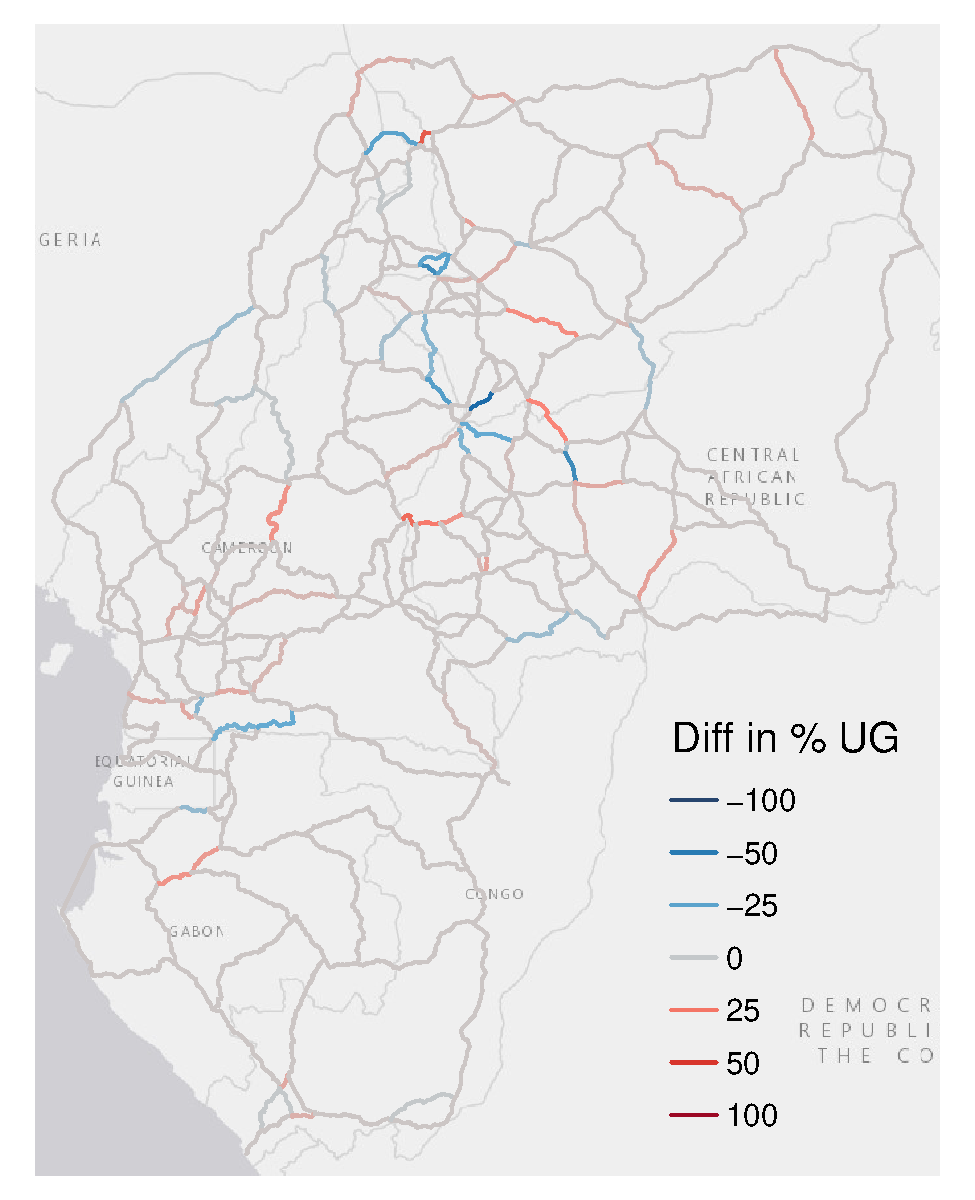
\includegraphics[width=0.48\textwidth]{"../figures/GE/trans_africa_network_GE_20g_5b_fixed_cgc_sigma3.8_rho2_julia_google_Ijk_bc_perc_ug_diff.pdf"}
\end{tabular}
}
% \raggedright
\scriptsize 
\emph{Notes:} Figure shows the welfare maximizing 5 billion USD'15 infrastructure spending on upgrading the network without border frictions (top) and with border frictions (bottom). Spending is indicated in terms of the \% of each link being upgraded. Under frictions (bottom) the difference to the frictionless case is shown.   
% \vspace{-10cm}
\end{figure}

\begin{figure}[h!] \vspace{-2mm}
\centering
\caption{\label{fig:GE_UG_5b} Welfare Maximizing Infrastructure Spending in GE: Building \& Upgrading Links (5B)}
\vspace{2mm}
\resizebox{\textwidth}{!}{
\begin{tabular}{cc}
5B Standard Planner & 5B Standard Planner: Frictions \\
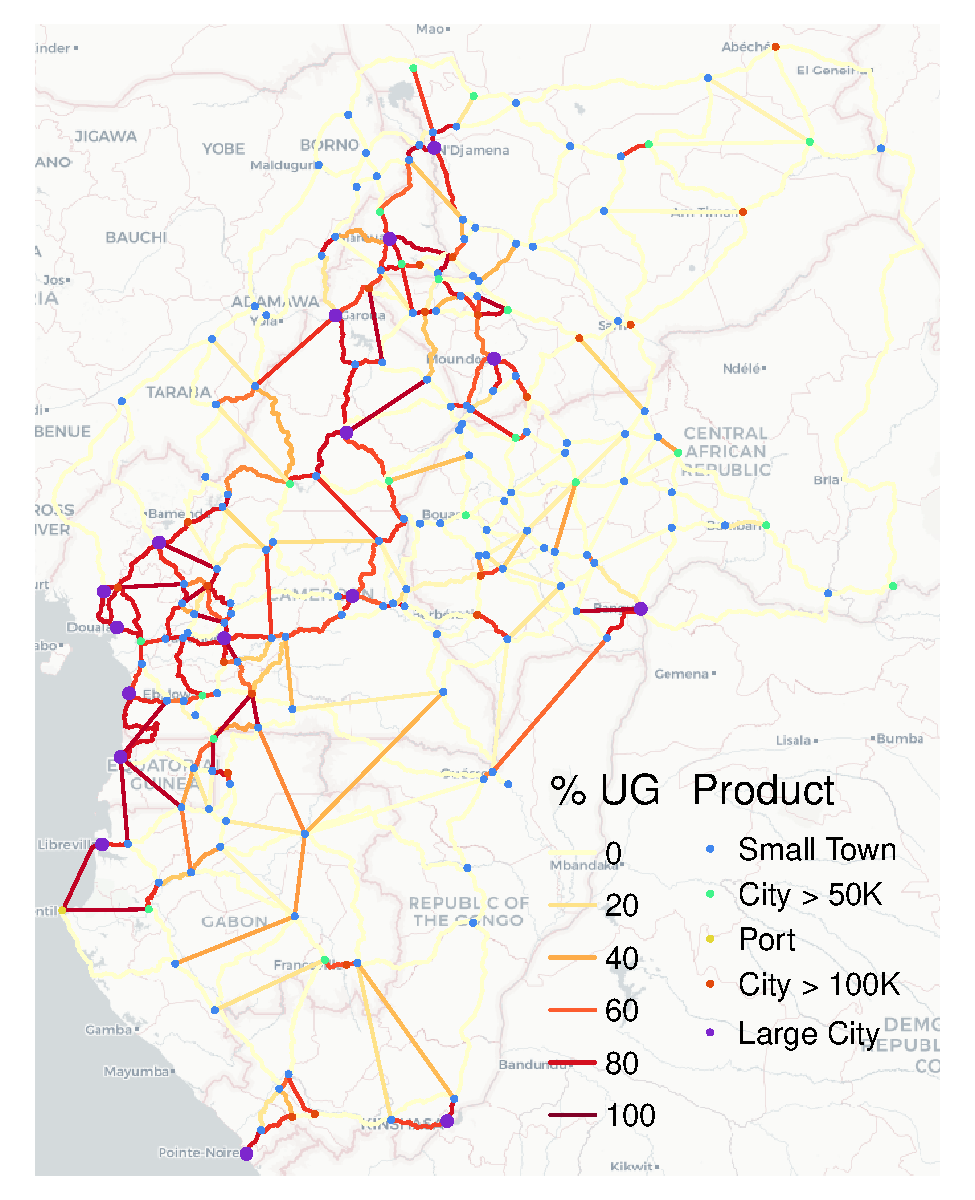
\includegraphics[width=0.48\textwidth]{"../figures/GE/trans_africa_network_GE_add_20g_5b_fixed_cgc_sigma3.8_rho0_julia_google_perc_ug.pdf"} &
 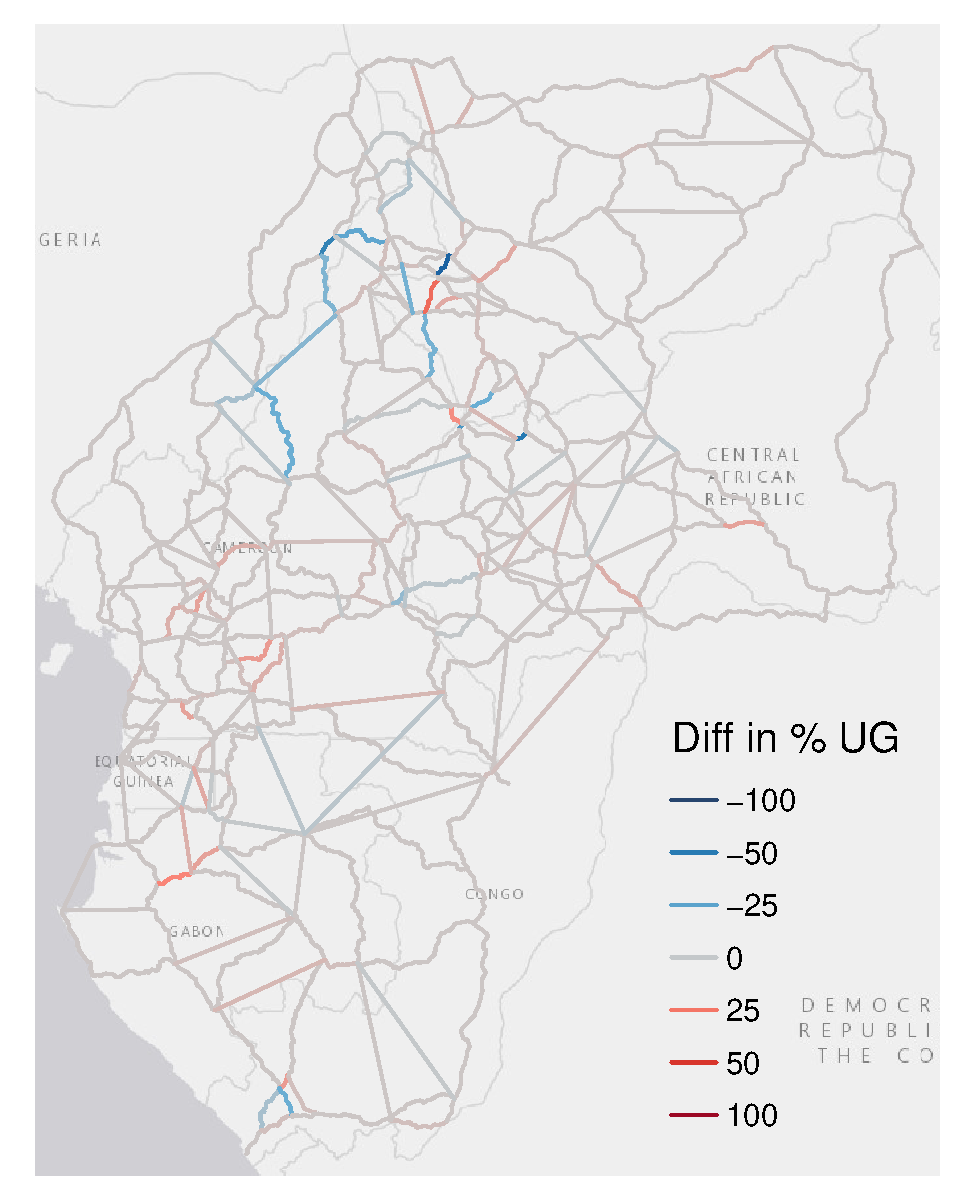
\includegraphics[width=0.48\textwidth]{"../figures/GE/trans_africa_network_GE_add_20g_5b_fixed_cgc_sigma3.8_rho0_julia_google_Ijk_bc_perc_ug_diff.pdf"} 
\end{tabular}
}
% \raggedright
\scriptsize 
\emph{Notes:} Figure shows the welfare maximizing 5 billion USD'15 infrastructure spending on upgrading the network with and without border frictions. Spending is indicated in terms of the \% of each link being upgraded. Under frictions the difference to the frictionless case is shown.   
% \vspace{-10cm}
\end{figure}


\begin{figure}[h!] \vspace{-8mm}
\centering
\caption{\label{fig:GE_UGNOfrFL} Flow of Goods under Optimal 2B Investments: Upgrading Links}
\vspace{2mm}
\begin{tabular}{c}
Standard Planner \\
\includegraphics[width=\textwidth]{"../figures/GE/trans_africa_network_GE_20g_2b_fixed_cgc_sigma3.8_rho0_julia_google_good_flows_4_city.pdf"} \\
Standard Planner: With Frictions \\
\includegraphics[width=\textwidth]{"../figures/GE/trans_africa_network_GE_20g_2b_fixed_cgc_sigma3.8_rho0_bc_julia_google_good_flows_4_city.pdf"} \\
Inequality Averse Planner \\
\includegraphics[width=\textwidth]{"../figures/GE/trans_africa_network_GE_20g_2b_fixed_cgc_sigma3.8_rho2_julia_google_good_flows_4_city.pdf"} \\
Inequality Averse Planner: With Frictions \\
\includegraphics[width=\textwidth]{"../figures/GE/trans_africa_network_GE_20g_2b_fixed_cgc_sigma3.8_rho2_bc_julia_google_good_flows_4_city.pdf"} 
\end{tabular}
% \raggedright
\scriptsize 
\emph{Notes:} Figure shows the flow of goods from selected cities under optimal 2B upgrading investments on a log scale. \\ \vspace{-20mm}
\end{figure}

\begin{figure}[h!] \vspace{-4mm}
\centering
\caption{\label{fig:GE_BUGNOfrFL} Flow of Goods under Optimal 1B-2B Investments: Building \& Upgrading Links}
\vspace{2mm}
\begin{tabular}{c}
1B Standard Planner \\
\includegraphics[width=\textwidth]{"../figures/GE/trans_africa_network_GE_add_20g_1b_fixed_cgc_sigma3.8_rho0_julia_google_good_flows_4_city.pdf"} \\
1B Standard Planner: With Frictions \\
\includegraphics[width=\textwidth]{"../figures/GE/trans_africa_network_GE_add_20g_1b_fixed_cgc_sigma3.8_rho0_bc_julia_google_good_flows_4_city.pdf"} \\
2B Standard Planner \\
\includegraphics[width=\textwidth]{"../figures/GE/trans_africa_network_GE_add_20g_2b_fixed_cgc_sigma3.8_rho0_julia_google_good_flows_4_city.pdf"} \\
2B Standard Planner: With Frictions \\
\includegraphics[width=\textwidth]{"../figures/GE/trans_africa_network_GE_20g_2b_fixed_cgc_sigma3.8_rho0_bc_julia_google_good_flows_4_city.pdf"} \\
\end{tabular}
% \raggedright
\scriptsize 
\emph{Notes:} Figure shows the flow of goods from selected cities under optimal 1B and 2B road building and upgrading investments on a log scale.
\end{figure}




\end{document}